% ISS presentation template
%
% Change history:
% 24.06.2010    Jürgen Ruoff        Initial creation
% 01.07.2010    Patrick Häcker      Generalization
% 02.07.2010    Patrick Häcker      Adjustment
% 15.11.2010    Patrick Häcker      Improvements
% 20.05.2011    Patrick Häcker      Add presentation type
% 06.01.2012	P. Hermannstädter 	Adapted to ISS, small mods

% Insert your name here
\newcommand{\presenter}{Zheming Yin}
\newcommand{\presentershort}{Zheming Yin}
\newcommand{\presenteremail}{st178328@stud.uni-stuttgart.de} 		% can be accessed using \presenteremail

% Insert presentation title here
\newcommand{\presentationtitle}{Range-Doppler map upsampling for single channel chirp sequence radar using Deep Learning}
\newcommand{\shortpresentationtitle}{Range-Doppler map upsampling}

% Insert type of presentation here (or comment line), probably one of:
% Mitarbeitervortrag, Bachelor-Arbeit, Master-Arbeit, Bachelor thesis, Master thesis
\newcommand{\presentationtype}{Master thesis}

% Insert presentation date here
\newcommand{\presentationdate}{24.04.2025}

% Uncomment the following line, if you write in English
% \newcommand{\lang}{german}
\newcommand{\lang}{english}

% Uncomment the following line, if you want to create handouts (setting to false does not work!)
%\newcommand{\handoutmode}{true}

% Load beamer class using LSS style
% Default \lang to ngerman
\ifx\lang\undefined
	\newcommand{\lang}{ngerman}
\fi

% Set \handout dependant on \handoutmode
\ifx\handoutmode\undefined
	\newcommand{\handout}{}
\else
	\newcommand{\handout}{handout}
\fi

% Make additional colors available
\PassOptionsToPackage{x11names}{xcolor}

% Load the beamer class, set the presentation data and use the LSS layout
\documentclass[\lang,\handout]{beamer}
\author[\presentershort]{\presenter}
\title[\shortpresentationtitle]{\presentationtitle}
\ifx \presentationtype \undefinded
\else
	\subtitle{\presentationtype}
\fi
\date{\presentationdate}
\institute{Institute of Signal Processing and\\ System Theory\\\vspace{1em}University of Stuttgart}
\usetheme[alternativetitlepage=true,% Use the fancy title page.
          titlepagelogo=isslogocolor,% Logo for the first page.
          watermark=isslogocolor,% Watermark used in every page.
          watermarkheight=25px,% Height of the watermark.
          ]{LSS}

% Grays uncovered objects instead of making them invisible; comment to make uncovered objects invisible
\setbeamercovered{transparent}

% Set work to presentation to not get blue hyperlinks
\newcommand{\work}{presentation}

% Input general definitions and loading of packages which can be shared with the thesis.
% Comment this line if you want to decide yourself which packages should be loaded.
% \def\me{Patrick Häcker}

% this is needed to get more resources to TeX - otherwise not all packages work at the same time
\usepackage{etex}

% ermöglicht ein if-then-else in LaTeX z. B. um Pakete variabel einzubinden
\usepackage{xifthen}
% \newcommand{\ifthen}[1]{\ifthenelse{#1}{}} % It does not work (behaviour is wrong)

% Load language specific things. Always load german, too, to get things like the long name of LSS correctly.
\ifx\lang\undefined
	\newcommand{\lang}{ngerman}
\fi
\ifthenelse{\equal{\lang}{german}}{
	\renewcommand{\lang}{ngerman}
}{}

\ifthenelse{\not\equal{\lang}{ngerman}}{
	\usepackage[ngerman,\lang]{babel}
}{
	\usepackage[\lang]{babel}
}

% damit man Umlaute direkt eingeben kann und diese erkannt werden (später auf utf8 umsteigen).
\usepackage[x-iso-8859-1]{inputenx}

% Umlaute werden als eine Einheit angesehen -> richtige Trennung und korrekt ins PDF eingebunden;
\usepackage[T1]{fontenc}

% Enthält gewisse Sonderzeichen wie z. B. Bullets
\usepackage{textcomp}

% Allow more set symbols (does not replace amsmath symbols if included before amsmath)
\usepackage[bbgreekl]{mathbbol}

% Schaltet AMS-Befehle, Schriftzeichen und Symbole frei (Mathepaket)
% Allow bold uppercase greek letters using the boldsymbol command
\usepackage{amsmath}
\usepackage{amsfonts}
\usepackage{amssymb}

% Allows bold italic uppercase letters
\usepackage{fixmath}



%Erlaubt den Seitenumbruch in Formeln, auch wenn er nach Möglichkeit vermieden wird
\allowdisplaybreaks[4]

% Enables fraction of the form a/b (with a nice slash)
\usepackage{nicefrac}

% Bindet die standardmäßig genutzten Times-Fonts ein (muss nach amsmath eingebunden werden)
% \usepackage{txfonts}

% Uses the Latin Modern font
\usepackage{lmodern}

% ermöglicht die aufrechte Schreibung griechischer Buchstaben
\usepackage{upgreek}

%ermöglicht das Einbinden von EPS-Dateien
\usepackage{graphicx}

%Das nachträgliche Ändern von Texten und Anpassen der Schriftart in EPS-Dateien beim Einbinden
\usepackage{psfrag}

%ermöglicht farbigen Text
\usepackage[x11names]{xcolor}

%ermöglicht farbige Tabellenhintergründe
\usepackage{colortbl}

% tikz is a cool drawing package using pgf
\usepackage{tikz}

\usetikzlibrary{3d,arrows,automata,backgrounds,calc,calendar,chains,decorations,decorations.footprints,decorations.fractals,decorations.markings,decorations.pathmorphing,decorations.pathreplacing,decorations.shapes,decorations.text,er,fadings,fit,folding,matrix,mindmap,patterns,petri,plothandlers,plotmarks,positioning,scopes,shadows,shapes.arrows,shapes.callouts,shapes,shapes.gates.logic.IEC,shapes.gates.logic.US,shapes.geometric,shapes.misc,shapes.multipart,shapes.symbols,through,topaths,trees}

% pgfplots enables the simple creation of plots from data points (eg. generated by matlab2tikz.m)
\usepackage{pgfplots}

% save every tikz plot as a pdf file (see package documentation of pgfplots)
% \usepgfplotslibrary{external}
% \tikzexternalize{ the main file name }

% If you want to print on a different size, use this package temporally
% \usepackage{pgfpages}
% \pgfpagesuselayout{resize}[a3paper]

% set PGF's decimal separator to comma for german documents
\ifthenelse{\equal{\lang}{ngerman}}{
	\pgfkeys{/pgf/number format/.cd, set decimal separator={{{,}}}}
}{}

% damit kann man Diagramme und Funktionen zeichnen
% \usepackage{pstricks,pst-plot,pst-node}
%\usepackage{pstricks-add}

% Zugriff auf gnuplot aus LaTeX heraus (erfordert -shell-escape bei latex-Aufruf)
% \usepackage{gnuplottex}

%\usepackage{multicol}

% Introduces \vref, a command which adds the page to the reference if necessary
\usepackage{nameref}
\usepackage{varioref}

\ifthenelse{\equal{\work}{thesis} \OR \equal{\work}{paper}}{
	\ifthenelse{\equal{\version}{computer}}{
		\def\colortype{color}
	}{}
	\ifthenelse{\equal{\version}{print}}{
		\def\colortype{black}
	}{}

	% Macht Links und Referenzen farbig und entfernt hässliche Kästchen drumherum
	% Hyperlinks blau ('color') (=PC-Version) oder schwarz ('black') (=Druckversion)
	\ifthenelse{\equal{\colortype}{color}}{
		\usepackage[breaklinks=true,colorlinks,linkcolor=blue]{hyperref}
	}{
		\usepackage[breaklinks=true]{hyperref}
	}
}
{
	\usepackage{hyperref}
}

% Makes the boolean ifpdf available to check if LaTeX is directly generating a PDF file


\usepackage{ifpdf}

\ifpdf
\else
	% Sorgt dafür, dass \url-Befehl automatische Umbrüche unterstützt (macht Probleme mit pdflatex)
	\usepackage{breakurl}
\fi

% Ermöglicht Abbildungen, die vom Text umflossen werden
% (zwei unterschiedliche Ansätze, haben wohl beide Nachteile)
% \usepackage{floatflt}
\usepackage{wrapfig}

% Setzt manche Bildunterschriften näher ans Bild heran, was schöner aussieht
\usepackage[hang]{caption}

% mehrere kleine Tabellen oder Grafiken aneinander anordnen (muss nach caption eingebunden werden)
%\usepackage{subfig}

%\usepackage{subfloat}

% Sauber formatierte Quellcode-Umgebung zur Verfügung stellen
\usepackage{listings}

% Ermöglicht Tabellen, deren Gesamtbreite eingestellt werden kann, wobei eine Spalte übrigen Platz bekommt
\usepackage{tabularx}

% Ermöglicht Tabellen, deren Gesamtbreite eingestellt werden kann, wobei übriger Platz prozentual aufgeteilt wird
\usepackage{tabulary}

% Erstellt schönere Tabellen, wobei vertikale Linien nicht mehr benutzt werden dürfen
\usepackage{booktabs}

% Ermöglicht Tabellenzellen die Ausdehnung über mehrere Zeilen
\usepackage{multirow}

% Writes an additional file to enable backward synchronisation between PDF and LaTeX
% "pdfsync uses extremely sensible code. You should not use pdfsync on final documents because
% it can change the layout rather significantly", yep, I hit a bug
% \usepackage{pdfsync}

% Ermöglicht das hinzufügen von fixme-Kommentaren, auch als \todo
\usepackage{fixme}
\newcommand{\todo}[1]{\fxwarning{#1}}
%\usepackage[inline,\status]{fixme}

% Ist für die Übergangsphase zu pdflatex sinnvoll, weil dann auch eps-Grafiken eingebunden werden können
%\usepackage{epstopdf}

% Abkürzungsverzeichnis erstellen und konfigurieren
%\usepackage[german,intoc]{nomencl}
%\renewcommand{\nomname}{Abkürzungsverzeichnis}
%\let\abbrev\nomenclature
%\setlength{\nomlabelwidth}{.15\hsize}
%\makenomenclature

% Stellt \doublespacing, \onehalfspacing und \singlespacing zur Verfügung
\usepackage{setspace}

% Allows putting two images on top of each other
% \usepackage[percent]{overpic}

% The savetrees package packs as much text as possible onto each page
% \usepackage{savetrees}

% Stellt das Kommando \extrarowheight für das glossaries-Paket zur Verfügung
\usepackage{array}

% allows usage of \degree
\usepackage{gensymb}

% Abkürzungen
% Sets
\newcommand{\Z}{\mathbb{Z}}
\newcommand{\N}{\mathbb{N}}
\newcommand{\Q}{\mathbb{Q}}
\newcommand{\R}{\mathbb{R}}
\newcommand{\C}{\mathbb{C}}

% differentiation
\newcommand{\del}{\partial}
\newcommand{\derivate}[2]{\frac{\del #1}{\del #2}}
\DeclareMathOperator{\dif}{d}
\DeclareMathOperator{\gradlong}{grad}
\DeclareMathOperator{\grad}{\bigtriangledown}

% statistics
\newcommand{\erw}[1]{\operatorname{E}\left(#1\right)}
\DeclareMathOperator{\E}{E}
\DeclareMathOperator{\prop}{P}
\DeclareMathOperator{\Var}{Var}
\DeclareMathOperator{\Cov}{Cov}
\DeclareMathOperator{\Bias}{Bias}
\DeclareMathOperator{\CRB}{CRB}

% linear algebra
\newcommand{\mat}[1]{\mathbf{#1}}
%\newcommand{\mat}[1]{\boldsymbol{#1}}
\newcommand{\Tr}[1]{\mathrm{Tr}\left( #1 \right)} %deprecated
\newcommand{\tr}[1]{\mathrm{tr}\left( #1 \right)}
\newcommand{\rang}[1]{\mathrm{rang}\left( #1 \right)}
\newcommand{\diag}[1]{\mathrm{diag}\left( #1 \right)}
\newcommand{\pinv}[1]{#1^{\dagger}}
\newcommand{\trans}[1]{#1^{\mathrm{T}}}
\newcommand{\hermitian}{\mathrm{H}}
\newcommand{\herm}[1]{#1^\mathrm{H}}
\newcommand{\konj}[1]{#1^{\mathrm{*}}}
\newcommand{\est}[1]{\hat{#1}}
\newcommand{\abs}[1]{\left\lvert#1\right\rvert}
\newcommand{\norm}[1]{\left\lVert#1\right\rVert}

% german abbreviations
\newcommand{\zB}{\mbox{z.\,B. }}
\newcommand{\iA}{\mbox{i.\,A. }}
\newcommand{\deha}{\mbox{d.\,h.\ }}
\newcommand{\oae}{\mbox{o.\,ä.\ }}
\newcommand{\uae}{\mbox{u.\,ä.\ }}
\newcommand{\oBdA}{\mbox{o.\,B.\,d.\,A. }}
\newcommand{\OBdA}{\mbox{O.\,B.\,d.\,A. }}
\newcommand{\ggf}{\mbox{ggf.\ }}
\newcommand{\vgl}{\mbox{vgl.\ }}
\newcommand{\evtl}{\mbox{evtl.\ }}
\newcommand{\bzw}{\mbox{bzw.\ }}
\newcommand{\bspw}{\mbox{bspw.\ }}
\newcommand{\ca}{\mbox{ca.\ }}

% english abbreviations
\newcommand{\eg}{\mbox{e.g.\ }}
\newcommand{\ie}{\mbox{i.e.\ }}

% quotes
\newcommand{\gq}[1]{\glq#1\grq}
\newcommand{\gqq}[1]{\glqq#1\grqq}
\newcommand{\eq}[1]{`#1'}
\newcommand{\eqq}[1]{``#1''}


% functions
\newcommand{\e}[1]{\operatorname{e}^{\,#1}}
\newcommand{\argmax}[2]{\underset{#1}{\operatorname{argmax}}\left( #2 \right)}
\newcommand{\argmaxima}[2]{\underset{#1}{\operatorname{argmaxima}}\left( #2 \right)}
\newcommand{\argmin}[2]{\underset{#1}{\operatorname{argmin}}\left( #2 \right)}
\DeclareMathOperator{\arc}{arc}
\DeclareMathOperator{\sinc}{sinc}
\DeclareMathOperator{\ggT}{ggT}
\DeclareMathOperator{\kgV}{kgV}
\DeclareMathOperator{\lcm}{lcm}

% symbols
% \newcommand{\degree}{\ensuremath{^\circ}}
\newcommand{\entspricht}{\mathrel{\hat{=}}}
\newcommand{\sollgleich}[0]{\overset{!}{=}}
\newcommand{\help}{\textcircled{\scriptsize{?}}}

% general
\newcommand{\op}[1]{\operatorname{#1}}
\newcommand{\smtext}[1]{{\scriptscriptstyle\text{#1}}}
%Zeilenumbruch mit eineinhalbzeiligem Abstand
\newcommand{\br}{\vspace{0.6em}\newline} %entspricht etwa \par\smallskip, geht aber auch in captions
\newcommand{\unit}[2]{\ensuremath{#1}\,\ensuremath{\mathrm{#2}}}
% \newcommand{\definition}[1]{\textit{#1}}
\newcommand{\includeplot}[1]{\centering\includegraphics{parent/Plots/#1.eps}}
\newcommand{\link}[1]{\href{#1}{\url{#1}}}
\newcommand{\shortlink}[1]{\href{#1}{#1}}
\newcommand{\mailto}[1]{\href{mailto:#1}{#1}}
\newcommand{\textlink}[2]{\href{#2}{\url{#1}}}
\newcommand{\vecfun}[2]{#1\hspace{-0.1em}\left(\vec #2\right)}
\newcommand{\equal}[1]{\overset{\text{#1}}{=}}
\newcommand{\matlab}{\textsc{Matlab}\raisebox{1ex}{\tiny{\textregistered}} }

% renews
\renewcommand{\inf}{\infty}
\renewcommand{\matrix}[1]{\mathbf{#1}}
\renewcommand{\j}{\mathrm{j}}
\renewcommand{\gcd}[0]{\operatorname{gcd}}
\renewcommand{\-}{\,--\,}


% Definiert den Befehl \writetofile, der als erstes Argument den Dateinamen und als zweiten Befehl den zu schreibenden Text erwartet
\newcommand{\writetofile}[2]{
% Erstelle Variable outfile
\newwrite\outfile
%Öffne Datei mit Handle outfile
 \immediate\openout\outfile=#1
%Schreibe in Datei
 \immediate\write\outfile{#2}
%Schließe Datei
\immediate\closeout\outfile
}

\newcommand{\readfromfile}[1]{
\newread\infile
\immediate\openin\infile=#1
\immediate\read\infile to \tempXBE
\immediate\closein\infile
\tempXBE
}


% \newcommand{\dotsnewline}{\mydotfill\,\linebreak.}

% Allgemeinerer Ansatz als Paket nomencl um mehrere Abkürzungs-/Symbolverzeichnisse zu erstellen
% Glossary "acronym" wird vordefiniert und Glorraries kommen in Inhaltsverzeichnis (toc)
% einsetzbar: toclike2, toclike3
%\usepackage[acronym,toc,style=toclike3acronym]{glossaries}
% deactivate toclike3acronym temporally due to squeeze upgrade

% Deactivated here and activated in main document, as makeglossaries does not work otherwise (WTF?)
% \usepackage[acronym,toc,style=listdotted]{glossaries}

% Abschließender Punkt in jeder Zeile wird weggelassen
% \renewcommand{\glspostdescription}{}
% Lässt Leerzeile bei Anfangsbuchstabenwechsel in den Verzeichnissen weg
% \renewcommand{\glsgroupskip}{}

% \newcommand{\newacronymdots}[2]{\newglossaryentry{#1}{type=\acronymtype, name={#1}, description={#2}, text={#1}, first={#2 (#1)}, plural={#1s}, firstplural={#2s (#1s)}, symbol={\dotsnewline}}}


% \newcount\boolcounter
% \boolcounter=1
% \advance\boolcounter by 1
% ermögliche Kennzeichnung eines Akronyms im Text durch \acronym{was}
%%%\newcommand{\acronym}[1]{\acr{#1}}
% \newcommand{\acronym}[1]{\gls{#1}}
% \let\acronym\gls
% \newcommand{\acronym}[1]{#1}
%\newcommand{\acronymnolink}[1]{\protect\acr*{#1}}
% ermöglicht die Benutzung eins Akronyms mit beliebigem Text (Argument #2)
% \newcommand{\acronymtext}[2]{\glslink{#1}{#2}}
% ermöglicht das Benutzen eines Akronyms, ohne dass die ausgeschriebene Version (dieses Mal) verwendet wird
% \newcommand{\acronymshort}[1]{\glslink{#1}{#1}}
% Verwendet ein Akronym ohne einen Link zu setzen (geht nicht in floating-Umgebungen)
%\newcommand{\acronymnolink}[1]{#1\glsadd{#1}}
% ermögliche Definition eines Akronyms in akronyme.tex durch \defineacronym{was}{wie}
% \newcommand{\defineacronym}[2]{\newacronym{#1}{#1}{#2}}
% \newcommand{\defineacronym}[2]{}
% \newcommand{\defineacronymdots}[2]{\newacronymdots{#1}{#2}}
%Sorgt dafür, dass man "\acronym{DoS}[-Angriff]" schreiben kann und dann automatisch "DoS-Angriff (Denial of Service)"
%geschrieben wird, bzw. "DoS-Angriff", je nachdem, ob es das erste Mal ist oder nicht
% \defglsdisplayfirst[acronym]{#3#4 (#2)}
% analog zu Akronymen: \definevar legt Symbol an, \var referenziert dieses
% \let\var\gls
% \newcommand{\var}[1]{#1}
% \newcommand{\var}[1]{\ifodd\boolcounter{%
% \protect\gls*{#1}%
% }\else%
% \text{\gls{#1}}\fi%
% }
%\newcommand{\varshort}[1]{\text{\glslink{#1}}\text{#1}}
%\newcommand{\varquiet}[1]{\glsadd{#1}}
%\newcommand{\definevar}[3]{\newglossaryentry{#1}{name=\ensuremath{#2},description={#3},sort=#1}}
\newcommand{\definevar}[4]{\newglossaryentry{#2}{name=\ensuremath{#3},description={#4},sort=#1}}
% \newcommand{\definevar}[4]{}
%\newcount\varcounter
%\varcounter=1
%\newcommand{\definevar}[3]{\definevariable{#1}{#2}{\arabic\varcounter #3}{\arabic\varcounter}}%{\arabic\varcounter}\advance\varcounter by 1}
%\newcommand{\definevariable}[4]{\newglossaryentry{#1}{name=\ensuremath{#2},description={#3},sort={#4}}\advance\varcounter by 1}
%\newcommand{\definevar}[4][\DefaultOpt]{%
%\def\DefaultOpt{#2}%
%\newglossaryentry{#2}{name=\ensuremath{#3},description={#1 wird sortiert #4},sort=#1}%
%\newglossaryentry{#2}{name=\ensuremath{#3},description={#4}}%
%}
% \newcommand{\varnolink}[1]{\protect\gls*{#1}}

% create glossaries internally (deactivated here, as this results in an error, must be activated in main file (WTF?))
% \makeglossaries

% \let\addtocontentsOld\addtocontents
% \renewcommand{\addtocontents}[2]{\advance\boolcounter by 1 \addtocontentsOld{#1}{#2} \advance\boolcounter by 1}

%Problem: Hochzahlen sitzen um Variablen mit Index unsauber, temporäre Lösung:
%\text{\glslink{thetaHatDNF}{$\hat{\vec{\theta}}_{\mathrm{DNF}}^3$}}
%anstatt:
%\var{thetaHatDNF}^3

% unknown hyphenation rules
\hyphenation{Im-puls-ant-wort Im-puls-ant-wort-ko-ef-fi-zien-ten
Pro-gramm-aus-schnitt Mi-kro-fon-sig-nal Sig-nal Rech-ner-ar-chi-tek-tur
Rech-ner-ar-chi-tek-tur-en Leucht-dich-te-mess-ka-me-ra Gam-ma-kor-rek-tur IEEE
Grund-an-nah-me}

% Definiert die Farbe Gray aus gray mit 80% Sättigung
\definecolor{Gray}{gray}{0.8}

%definiert deutsche hyperref-Bezeichner so um, dass \autoref problemlos funktioniert
% \ifthenelse{\equal{\lang}{ngerman}}{
% 	\addto\extrasngerman{%
% 		\def\appendixautorefname{Anhang}%
% 		\def\chapterautorefname{Kapitel}%
% 		\def\equationautorefname{Gleichung}%
% 		\def\itemautorefname{Punkt}%
% 		\def\pageautorefname{Seite}%
% 		\def\partautorefname{Teil}%
% 		\def\sectionautorefname{Kapitel}%
% 		\def\subsectionautorefname{Kapitel}%
% 		\def\figureautorefname{Abbildung}%
% 		\def\footnoteautorefname{Fußnote}%
% 		\def\tableautorefname{Tabelle}%
% 	}
% }{
% 	\addto\extrasngerman{%
% 		\def\appendixautorefname{Appendix}%
% 		\def\chapterautorefname{Chapter}%
% 		\def\equationautorefname{Equation}%
% 		\def\itemautorefname{Item}%
% 		\def\pageautorefname{Page}%
% 		\def\partautorefname{Part}%
% 		\def\sectionautorefname{Chapter}%
% 		\def\subsectionautorefname{Chapter}%
% 		\def\figureautorefname{Figure}%
% 		\def\footnoteautorefname{Footnote}%
% 		\def\tableautorefname{Table}%
% 	}
% }


% define autoref to act like eqref for equations
\makeatletter
\@ifdefinable\equationname{%
\let\equationname\equationautorefname%
}
\addto\extrasenglish{%
\def\equationautorefname~#1\@empty\@empty\null{(#1\@empty\@empty\null)}
}
% \addto\extrasngerman{%
% \def\equationautorefname~#1\@empty\@empty\null{\equationname~(#1\@empty\@empty\null)}
% }
\makeatother

% Use serifs in math environment and no serifs in text environment
\usefonttheme[onlymath]{serif}

% Define two practical lengths, which can be uses when setting the size of graphics
\newlength\fullwidth
\setlength\fullwidth{11cm}
\newlength\fullheight
\setlength\fullheight{6.8cm}

% Set lines a bit thicker in presentations when using pgfplots to allow recognition of colored lines
\ifx\pgfplotsset\undefined
	%
\else
	\pgfplotsset{every axis/.append style={thick}}
\fi

% Put four slides on each page if handout mode activated
\ifx\handoutmode\undefined
	%
\else
	\usepackage{pgfpages}
	\pgfpagesuselayout{4 on 1}[a4paper,border shrink=5mm,landscape]
	% use this line instead, if you have problems with rotated eps files
	% \pgfpagesuselayout{4 on 1}[border shrink=5mm,landscape]
\fi


% Define Layout parameters:
\setlength{\itemsep}{0.5em}


\documentclass{beamer}
\usepackage{setspace}
\usepackage[sorting=none]{biblatex}
\addbibresource{refs.bib}
\usepackage{graphicx}
\usepackage{caption}
\captionsetup[figure]{labelformat=simple, labelsep=period}
\newcounter{section}
\setcounter{section}{0}
\renewcommand{\thefigure}{\thesection.\arabic{figure}}
\usepackage{animate}
\setbeamertemplate{caption}[numbered]
\renewcommand{\thetable}{\thesection.\arabic{table}}
\renewcommand{\tablename}{Table}
\AtBeginDocument{
  \renewcommand{\tablename}{Table}
}



% My commands:

% -----------------------------------------------------------------------------
% -----------------------------------------------------------------------------
\begin{document}
\lstset{basicstyle=\small\ttfamily,xleftmargin=15pt,language=Matlab,
        commentstyle=\color{green},showstringspaces=false,stringstyle=\color{magenta}\ttfamily}

\renewcommand{\figurename}{Figure}

% -----------------------------------------------------------------------------
% This is the title page
\begin{frame}[t,plain]
	\titlepage
\end{frame}


% % -----------------------------------------------------------------------------
% % Motivation slide
% \begin{frame}[t]{Motivation}
% \uncover<1->{
% 	\lstinline">> why"\\
% 	\lstinline"To fool the tall good and smart system manager."}
% \only<2->{
% 	\begin{figure}
% %		\includegraphics[width=\textwidth]{ }
% 	% Images: 	pdflatex can handle png jpg pdf and so on directly, but no eps
% 	%			latex and dvi2ps ps2pdf can handle eps and eventually png pdf or jpg if you provide a bounding box
	
% 	\end{figure}
% }

% \end{frame}


% -----------------------------------------------------------------------------
% Introduction slide
\begin{frame}[t]{Introduction}
    \begin{itemize}
    	\item Single channel chirp sequence radar
        \vspace{0.5\baselineskip}
        \item Range-Doppler map upsampling
        \vspace{1.0\baselineskip}
            \begin{figure}
                \centering
                \hspace*{-0.5cm}
                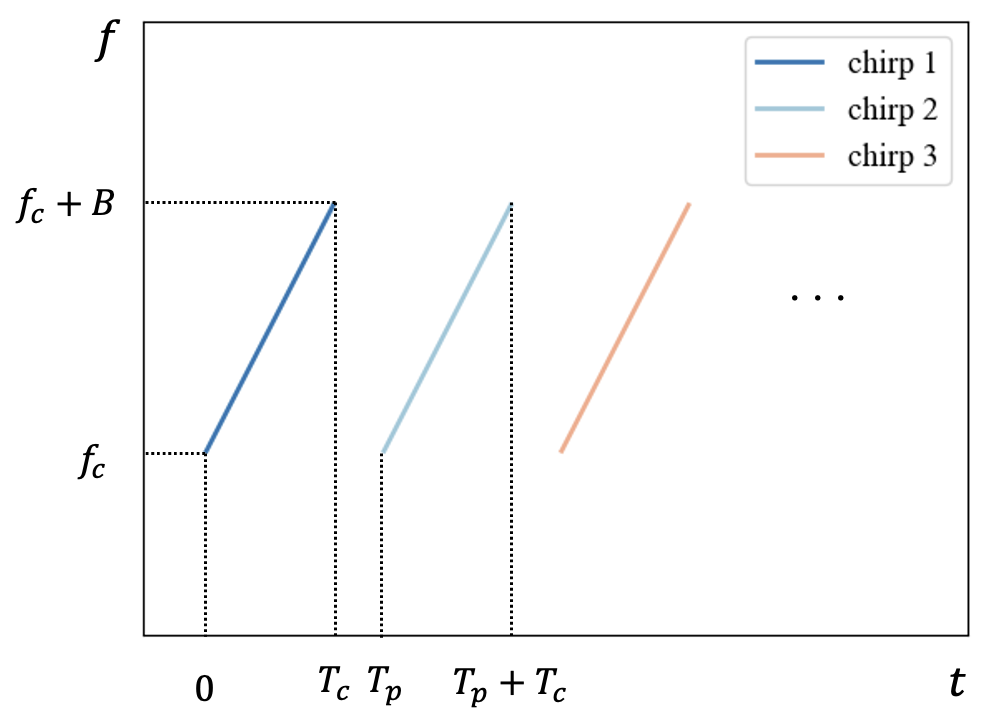
\includegraphics[scale=.32]{MA_presentation/figures/chirp_sequence_radar.png}
                \caption{The principle of the chirp sequence radar based on the frequency modulated continuous wave (FMCW) radar}
            \end{figure}
    \end{itemize}

\end{frame}


% -----------------------------------------------------------------------------
% Motivation slide
\begin{frame}[t]{Motivation}

    \begin{itemize}
        \item<2-> Importance in the indoor localization
    	\item<2-> Limited resolution by the radar system, cost, regulation, etc.
        \item<2-> Specified for the range-Doppler map
        \item<2-> Wide dynamic range of the amplitude
    \end{itemize}

    \vfill

    \only<1->{
    \begin{figure}
        \centering
        \hspace*{-1cm}
        \begin{minipage}{0.45\textwidth}
            \centering
            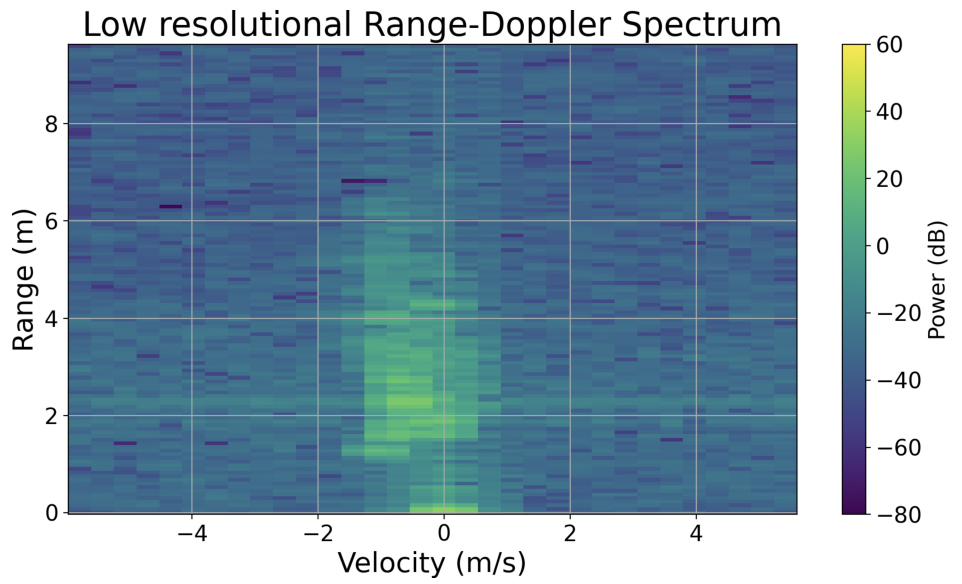
\includegraphics[height=0.73\textwidth]{MA_presentation/figures/factor_2_new.png}
            % \caption{Low-resolution with the factor 2}
        \end{minipage}
        \begin{minipage}{0.45\textwidth}
            \centering
            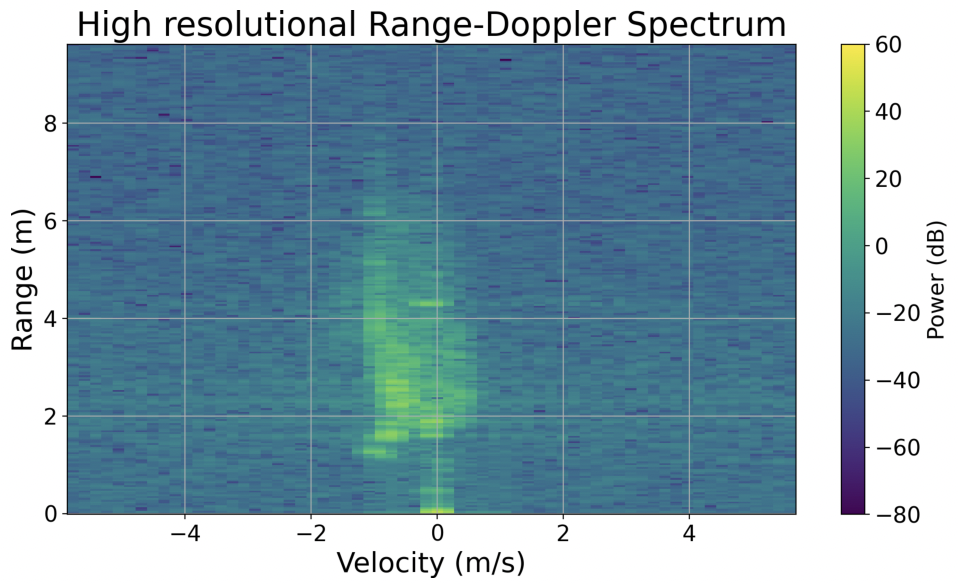
\includegraphics[height=0.73\textwidth]{MA_presentation/figures/high_res_new.png}
            % \caption{High-resolution}
        \end{minipage}
        \caption{An example of the paired low-resolution and high-resolution range-Doppler maps.}
    \end{figure}
    }

\end{frame}


% -----------------------------------------------------------------------------
% This is the table of contents. You can insert a motivation before or after this slide.
\begin{frame}
	\ifthenelse{\equal{\lang}{ngerman}}{
		\frametitle{Inhaltsverzeichnis}
	}{
		\frametitle{Table of Contents}
	}
	\tableofcontents
\end{frame}

% Add an extra slide at the beginning of each section while highlighting the current section
% Use \section* to skip the slide once or comment the following to skip all overview slides.
\AtBeginSection[]
{
	\begin{frame}<beamer>
		\ifthenelse{\equal{\lang}{ngerman}}{
			\frametitle{Inhaltsverzeichnis}
		}{
			\frametitle{Table of Contents}
		}
% 		\frametitle{\contentsname}
		\tableofcontents[currentsection]
	\end{frame}
}




%% ===================================================================
\section{Dataset}
\subsection{Dataset collection}
\setcounter{section}{1}
\setcounter{figure}{0}
% --------------------------------------------------------------------

% \begin{frame}[t]{Hardware \& Initialization}
% 	\begin{columns}[t,onlytextwidth]
% 		\column<1->{.5\textwidth}
%             \begin{figure}
%                 \centering
%                 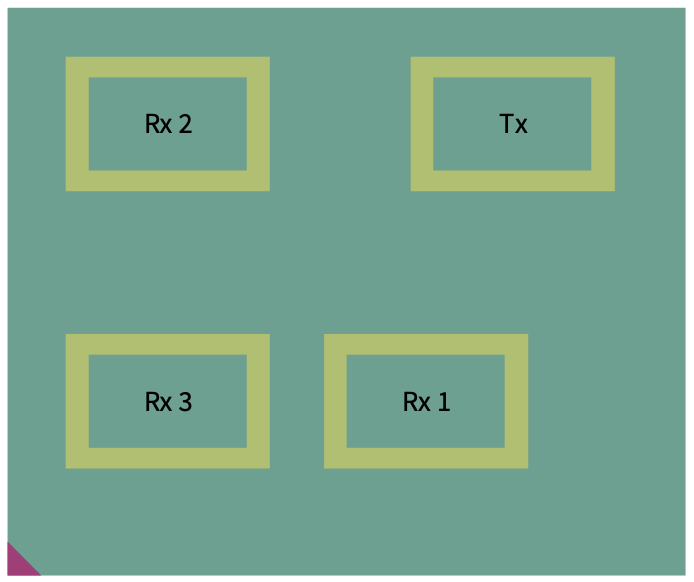
\includegraphics[scale=.43]{MA_presentation/figures/antenna arrangement.png}
%                 \caption{Antennas arrangement of the BGT60TR13C radar from Infineon \cite{ag_bgt60tr13c_nodate}}
%             \end{figure}
% 		\column<2->{.5\textwidth}	
% 		\begin{itemize}
%             \vspace{0.5\baselineskip}
% 			\item \#Chirps $N_c = 64$
% 			\item \#Samples of chirp $N_s=512$
%             \item Shape (512, 64)
% 			\item Maximum range $r_{max} = 9.6\,\mathrm{m}$
%             \item Range resolution $\Delta r = 0.075\,\mathrm{m}$
% 			\item Maximum velocity $v_{max} = 5.68\,\mathrm{m/s}$
% 			\item Velocity resolution $\Delta v = 0.355\,\mathrm{m/s}$
% 		\end{itemize}	
% 	\end{columns}	
% \end{frame}


\begin{frame}[t]{Hardware \& Initialization}
	\begin{columns}[t,onlytextwidth]
		\column<1->{.43\textwidth}
            \begin{figure}
                \vspace{-0.3\baselineskip}
                \centering
                \hspace{-0.5cm}
                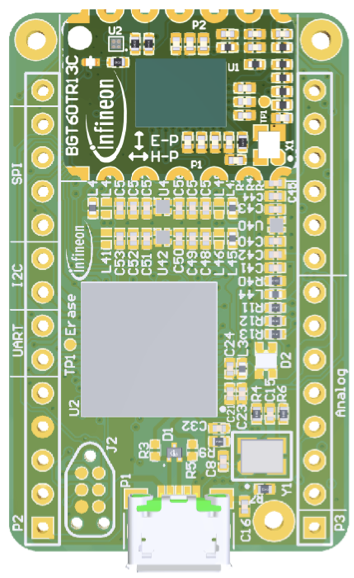
\includegraphics[scale=.55]{MA_presentation/figures/radar_hardware.png}
                \caption{BGT60TR13C radar from Infineon \cite{ag_bgt60tr13c_nodate}}
            \end{figure}
		\column<2->{.57\textwidth}	
		\begin{itemize}
            \vspace{0.6\baselineskip}
			\item \#Chirps $N_c = 64$
			\item \#Samples of chirp $N_s=512$
            \item Shape (512, 64)
			\item Maximum range $r_{max} = 9.6\,\mathrm{m}$
            \item Range resolution $\Delta r = 0.0375\,\mathrm{m}$
			\item Maximum velocity $v_{max} = 5.68\,\mathrm{m/s}$
			\item Velocity resolution $\Delta v = 0.178\,\mathrm{m/s}$
		\end{itemize}	
	\end{columns}	
\end{frame}


% \begin{frame}[t]{Collection}
% 	\begin{columns}[t,onlytextwidth]
% 		\column<1->{.65\textwidth}
%             \begin{figure}
%                 \centering
%                 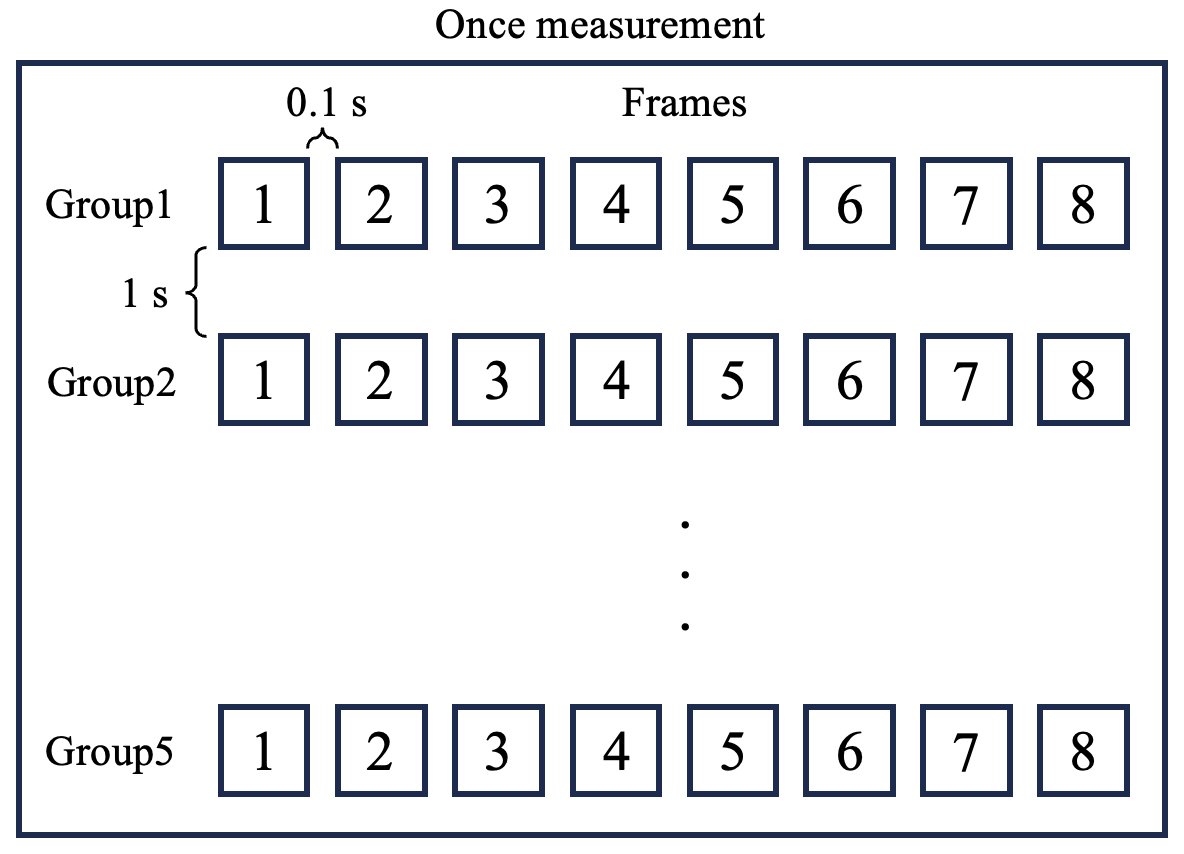
\includegraphics[scale=.33]{MA_presentation/figures/dataset_collection.png}
%                 \caption{Structure of the collection}
%             \end{figure}
% 		\column<2->{.35\textwidth}	
% 		\begin{itemize}
%             \vspace{1.2\baselineskip}
% 			\item Corridor environment
% 			\item Dynamic
%             \item Different tempos
% 			\item Different direction
% 			\item 2,362 Measurements
% 			\item Size 16.4 GB
% 		\end{itemize}	
% 	\end{columns}	
% \end{frame}

\begin{frame}[t]{Collection}

    % \only<1->{
    \begin{figure}
        \centering
        \hspace*{-1cm}
        \begin{minipage}{0.25\textwidth}
            \centering
            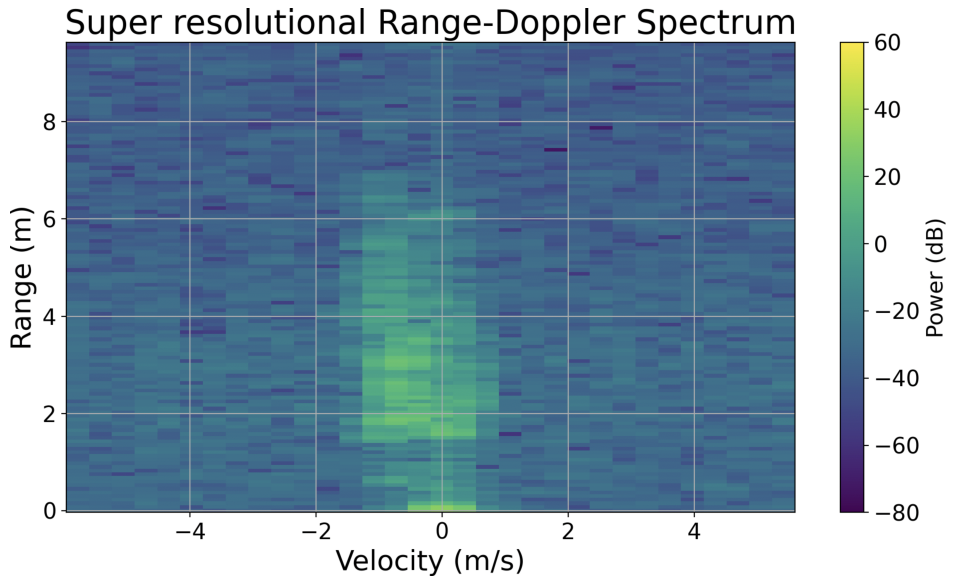
\includegraphics[height=0.75\textwidth, keepaspectratio]{MA_presentation/figures/frame1.png}
            \caption*{\hspace{0.25cm}Frame1}
        \end{minipage}
        \begin{minipage}{0.25\textwidth}
            \centering
            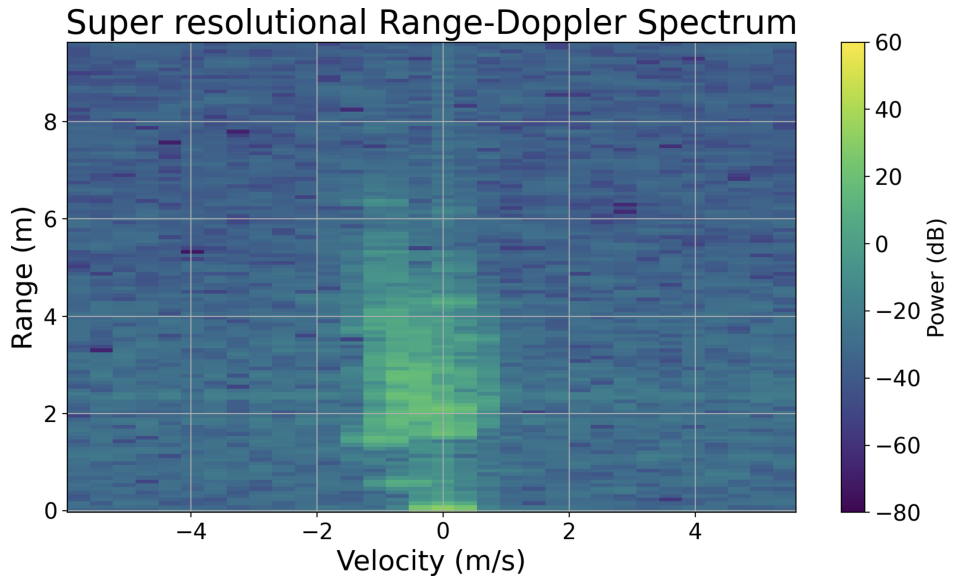
\includegraphics[height=0.75\textwidth]{MA_presentation/figures/frame2.png}
            \caption*{\hspace{0.29cm}Frame2}
        \end{minipage}
        \begin{minipage}{0.25\textwidth}
            \centering
            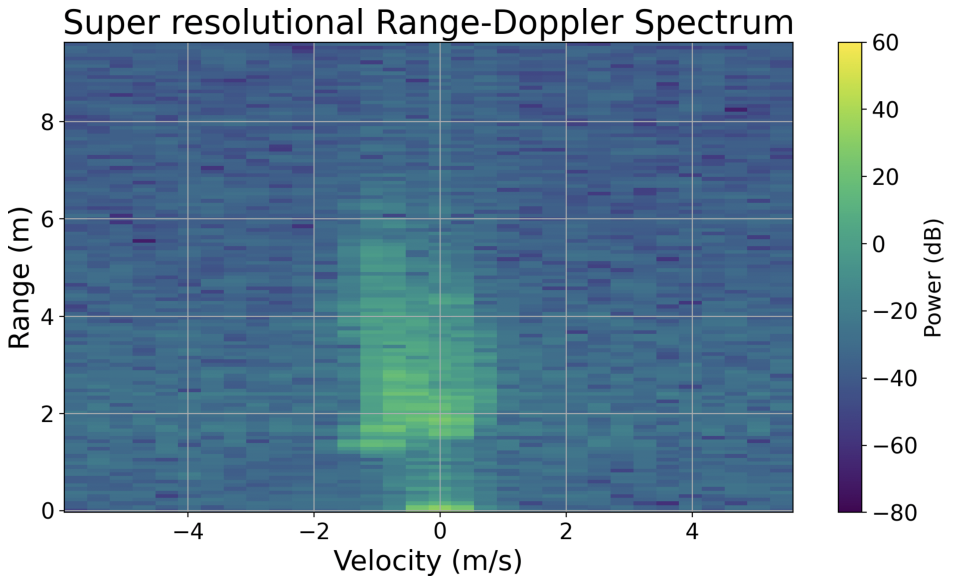
\includegraphics[height=0.75\textwidth]{MA_presentation/figures/frame3.png}
            \caption*{\hspace{0.25cm}Frame3}
        \end{minipage}
        \begin{minipage}{0.25\textwidth}
            \centering
            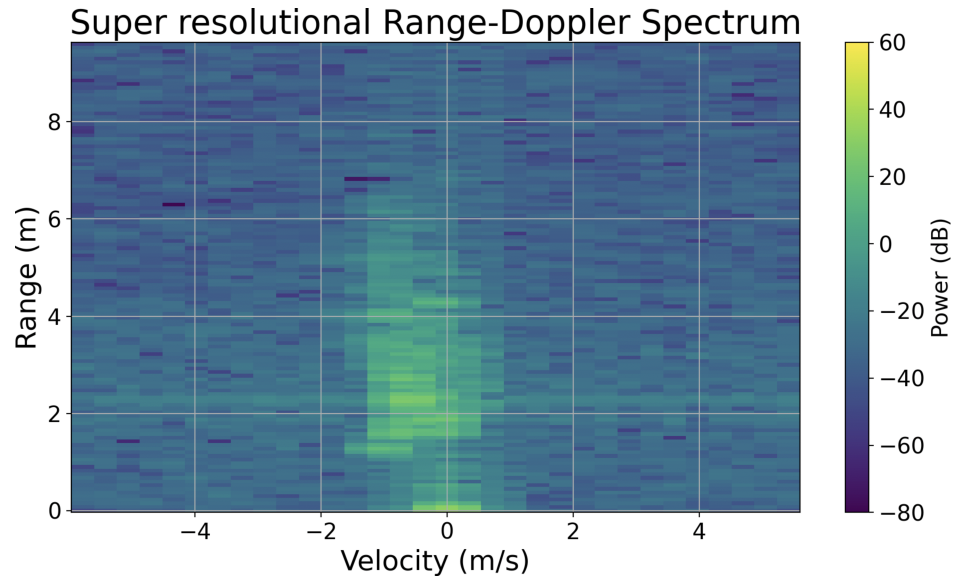
\includegraphics[height=0.75\textwidth]{MA_presentation/figures/frame4.png}
            \caption*{\hspace{0.29cm}Frame4}
        \end{minipage}
        \vspace{-0.3cm}
        \caption{Consecutive frames during the collection}
    \end{figure}
    % }

    % \vfill
    \vspace{-0.6\baselineskip}

    % \only<2->{
    \begin{columns}[t,onlytextwidth]
		\column{.5\textwidth}
        \begin{itemize}
            % \vspace{0.6\baselineskip}
			\item Corridor environment
			\item Over 90,000 frames
            \item Size 16.4 GB
		\end{itemize}
		\column{.5\textwidth}
		\begin{itemize}
            % \vspace{0.6\baselineskip}
			\item Dynamic motion
			\item Different tempos
            \item Different directions
		\end{itemize}	
	\end{columns}
    % }
    
\end{frame}



\subsection{Dataset loading}
% --------------------------------------------------------------------

% \begin{frame}[t]{Dataset loading}
%     \begin{itemize}
%     	\item TensorFlow Records (TFRecord) files creating
%         \vspace{0.5\baselineskip}
%         \begin{itemize}
%             \item Number of frames
%             \vspace{0.5\baselineskip}
%             \item Resampling
%         \end{itemize}
%         \vspace{1.0\baselineskip}
%         \item TFRecord files reloading
%         \vspace{0.5\baselineskip}
%         \begin{itemize}
%             \item Range-Doppler processing (RDP)
%         \end{itemize}
        
%     \end{itemize}

% \end{frame}



% \begin{frame}[t]{Sliding window for frames}
%     \begin{itemize}
%         \item Additional consecutive information
%         \vspace{0.5\baselineskip}
%         \item The last frame within each window to be upsampled
%         \vspace{0.5\baselineskip}
%         \item The number of frames in ground truth always as 1

%     \end{itemize}
    
%     \vspace{2.0\baselineskip}

%     % \begin{figure}
%     %     \centering
%     %     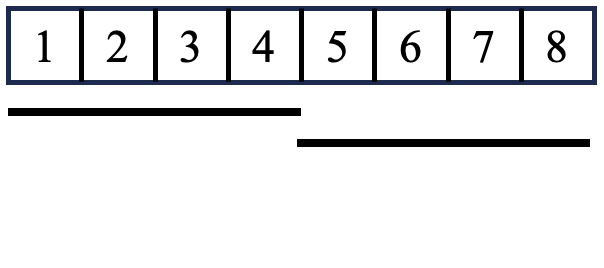
\includegraphics[scale=.6]{MA_presentation/figures/sliding_window_right.png}
%     %     \vspace{-5ex}
%     %     \caption{Sliding window with the length of 4 frames}
%     % \end{figure}

%     \begin{figure}
%         \centering
%         \begin{minipage}{0.49\textwidth}
%             \centering
%             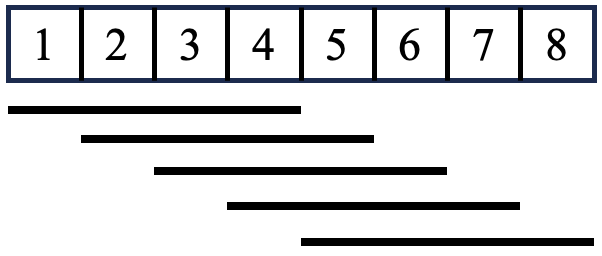
\includegraphics[height=0.4\textwidth]{MA_presentation/figures/sliding_window_left.png}
%         \end{minipage}
%         % \hspace{0.3cm}
%         \begin{minipage}{0.49\textwidth}
%             \centering
%             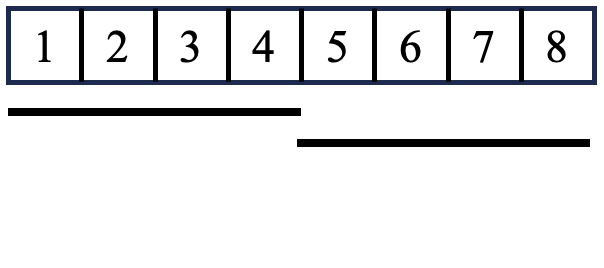
\includegraphics[height=0.4\textwidth]{MA_presentation/figures/sliding_window_right.png}
%         \end{minipage}
%         \caption{Sliding window with the length of 4 frames}
%     \end{figure}

% \end{frame}





\begin{frame}[t]{Resampling}
    \vspace{-1.5\baselineskip}
    \begin{columns}[t]
		\column{.45\textwidth}
        \begin{itemize}
            \item Range resolution
                \begin{equation}
                    \centering
                    \Delta r = \frac{c}{2B}
                \end{equation}
            \item Velocity resolution
                \begin{equation}
                    \centering
                    \Delta v = \frac{c}{2f\textsubscript{c}} \cdot \frac{1}{T\textsubscript{p} \cdot N\textsubscript{c}}
                \end{equation}
		\end{itemize}
		\column{.45\textwidth}	
		\begin{itemize}
            % \vspace{0.5\baselineskip}
			\item Maximum range
                \begin{equation}
                    \centering
                    r\textsubscript{max} = \frac{c \cdot F\textsubscript{s}}{2S}
                \end{equation}
			\item Maximum velocity
                \begin{equation}
                    \centering
                    v\textsubscript{max} = \frac{\lambda}{4 \cdot T\textsubscript{p}}
                \end{equation}
		\end{itemize}
	\end{columns}

    % \vspace{2.0\baselineskip}

    \begin{figure}
        \centering
        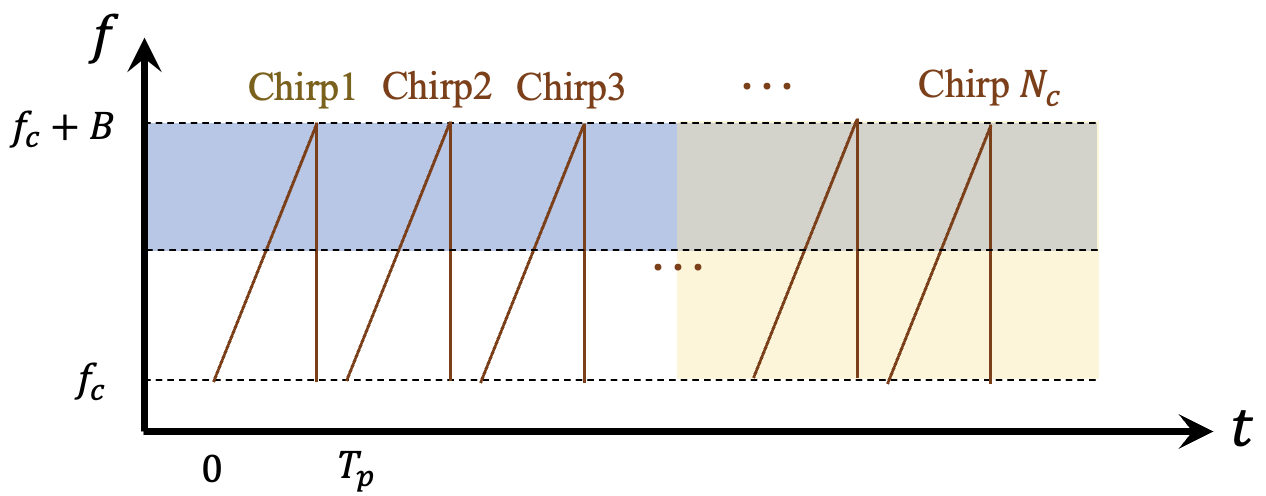
\includegraphics[scale=.4]{MA_presentation/figures/resampling.png}
        \vspace{-0.5ex}
        \caption{Downsampling by factor 2}
    \end{figure}

\end{frame}


\begin{frame}[t]{Range-Doppler processing (RDP)}
    \begin{itemize}
        \item Real-valued fast Fourier transform (rFFT) on range axis
        \begin{itemize}
            \vspace{0.2\baselineskip}
            \item Keep the positive frequency part and an offset
        \end{itemize}
        \vspace{0.2\baselineskip}
        \item Fast Fourier transform (FFT) on velocity axis
        \vspace{0.2\baselineskip}
        \item High-resolution shape from (512, 64) to (257, 64)
        \vspace{0.2\baselineskip}
        \item Low-resolution shape from (256, 32) to (129, 32)
    \end{itemize}

    \vspace{0.3\baselineskip}

    \begin{figure}
        \centering
        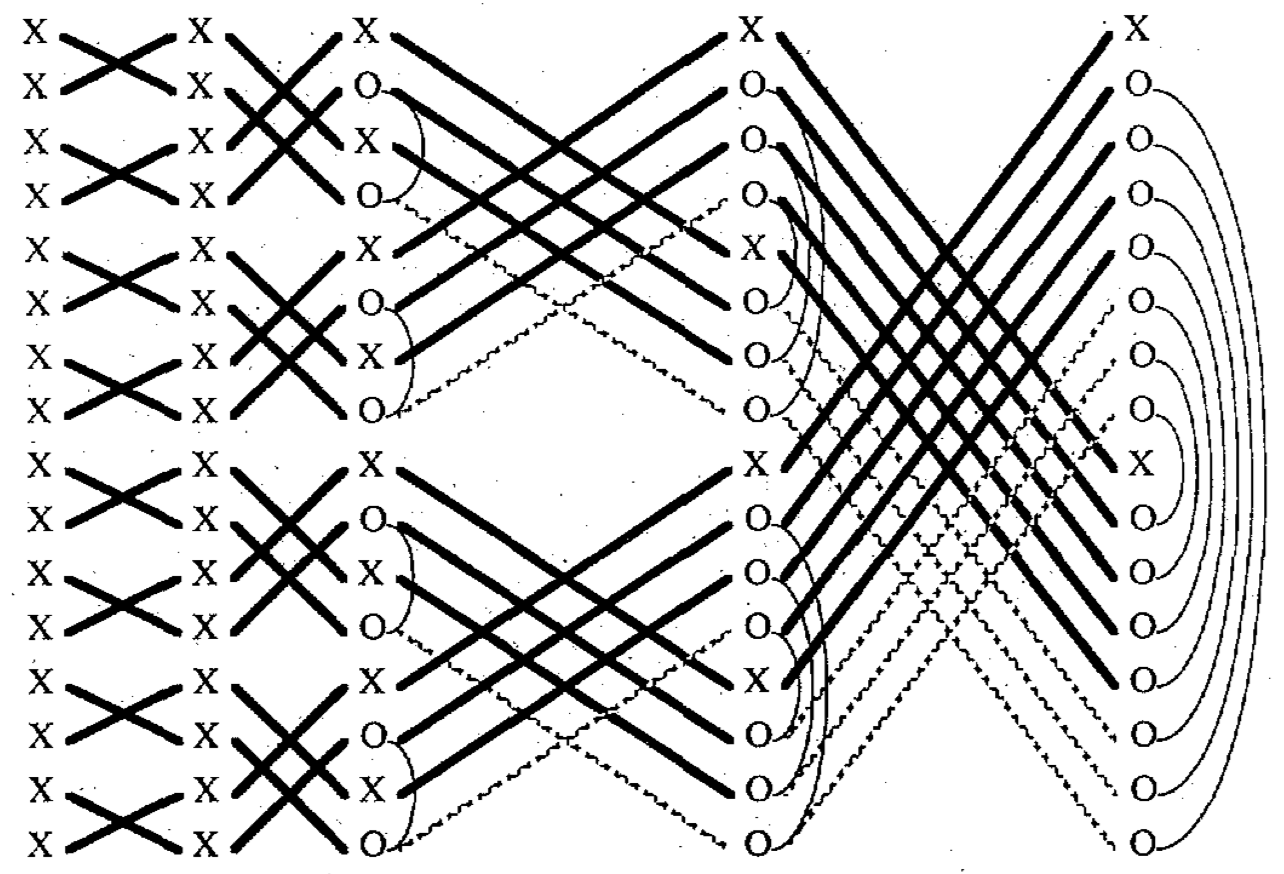
\includegraphics[scale=.27]{MA_presentation/figures/rfft.png}
        \caption{Overview of the FFT in the case of real-valued inputs \cite{sorensen_real-valued_1987}}
    \end{figure}

\end{frame}



\subsection{Dataset processing}
% --------------------------------------------------------------------

\begin{frame}[t]{Dataset processing}
    \begin{itemize}
    	\item Input data representation
            \begin{itemize}
                \vspace{0.2\baselineskip}
                \item Real and imaginary representation
                \vspace{0.2\baselineskip}
                \item Amplitude representation
                \vspace{0.2\baselineskip}
                \item Amplitude and phase representation
            \end{itemize}
        \vspace{0.5\baselineskip}
        \item Logarithm
            % \begin{itemize}
            %     \vspace{0.2\baselineskip}
            %     \item No logarithm on amplitude
            %     \vspace{0.2\baselineskip}
            %     \item Logarithm with base 10 on amplitude
            % \end{itemize}
        \vspace{0.5\baselineskip}
        \item Normalization
            \begin{itemize}
                % \vspace{0.2\baselineskip}
                % \item No normalization
                \vspace{0.2\baselineskip}
                \item Normalization on the amplitude
                \begin{equation}
                    \centering
                    \text{normalized data} = \frac{\text{data}}{\text{max}}
                \end{equation}
                \begin{equation}
                    \centering
                    \text{normalized data} = \frac{\text{data - min}}{\text{max - min}}
                \end{equation}
                \vspace{0.2\baselineskip}
                \item Normalization on the phase
                % $\text{normalized angle} = \frac{\text{angle}}{\pi}$
            \end{itemize}
    \end{itemize}

\end{frame}


%% ===================================================================
\section{Models}
\subsection{Dimension processing layer}
\setcounter{section}{2}
\setcounter{figure}{0}
% --------------------------------------------------------------------

\begin{frame}[t]{Dimension processing layer}
    \begin{itemize}
    	\item No dimension processing layer
            \begin{itemize}
                \vspace{0.2\baselineskip}
                \item Low-resolution shape keeps (129, 32)
                \vspace{0.2\baselineskip}
                \item After upsampling, shape from (129 , 32) to (258, 64)
                \vspace{0.2\baselineskip}
                \item Discard last sample, from (258, 64) to (257, 64)
            \end{itemize}
        \vspace{0.5\baselineskip}
        \item Padding along the range axis
            \begin{itemize}
                \vspace{0.2\baselineskip}
                \item Low-resolution shape from (129, 32) to (130, 32)
                \vspace{0.2\baselineskip}
                \item After upsampling, shape from (130 , 32) to (260, 64)
                \vspace{0.2\baselineskip}
                \item Discard last three samples, from (260, 64) to (257, 64)
            \end{itemize}
        \vspace{0.5\baselineskip}
        \item Convolutional layer with kernel size (2, 1) and stride 1
            \begin{itemize}
                \vspace{0.2\baselineskip}
                \item Low-resolution shape from (129, 32) to (128, 32)
                \vspace{0.2\baselineskip}
                \item After upsampling, shape from (128 , 32) to (256, 64)
                \vspace{0.2\baselineskip}
                \item Transposed convolutional layer from (256, 64) to (257, 64)
            \end{itemize}
    \end{itemize}

\end{frame}



\subsection{Upsampling layer}
% --------------------------------------------------------------------

\begin{frame}[t]{Upsampling layer}
    \begin{itemize}
    	\item Transposed convolutional layer
        \vspace{0.5\baselineskip}
        \item Pixel shuffle layer (depth-to-space method)
        \begin{itemize}
            \vspace{0.3\baselineskip}
            \item Shape from (N, C$\times$r\textsuperscript{2}, H, W) to (N, C, H$\times$r, W$\times$r)
        \end{itemize}
    \end{itemize}

    \vspace{0.5\baselineskip}

    \begin{figure}
        \centering
        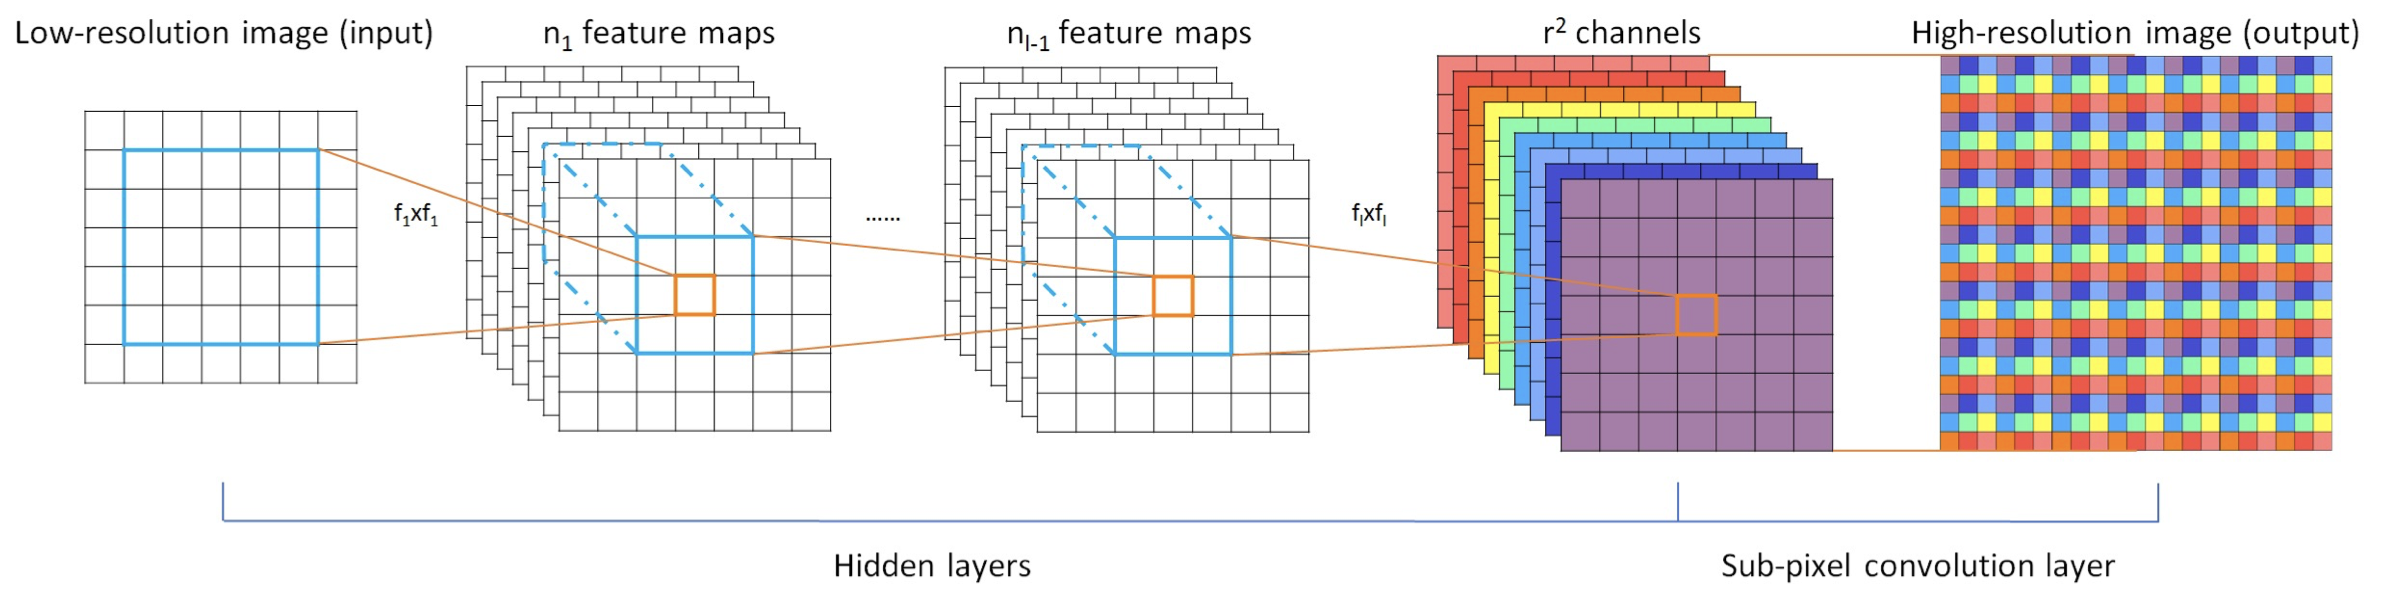
\includegraphics[scale=.27]{MA_presentation/figures/pixelShuffle.png}
        \caption{Pixel shuffle layer \cite{shi_real-time_2016}}
    \end{figure}

\end{frame}


\subsection{Multiple models}
% --------------------------------------------------------------------

% \begin{frame}[t]{Multiple models}
%     \begin{itemize}
%         \item Interpolation model
%         \vspace{0.5\baselineskip}
%     	\item Convolutional neural network (CNN) model
%         \vspace{0.5\baselineskip}
%         \item U-Net (UNet) model
%         \vspace{0.5\baselineskip}
%         \item UNet concat model \cite{prabhakara_high_2023}
%         \vspace{0.5\baselineskip}
%         \item Dual-Path Time-Frequency (DP-TF) Transformer model \cite{hinderer_blind_2022}
%         \vspace{0.5\baselineskip}
%         \item Image restoration with Swin Transformer (SwinIR) architecture \cite{liang_swinir_2021}
%             \begin{itemize}
%                 \vspace{0.3\baselineskip}
%                 \item SwinIR+Swin: With shifted window Transformer block
%                 \vspace{0.3\baselineskip}
%                 \item SwinIR+DP: With DP-TF Transformer block
%             \end{itemize}
%         \vspace{0.5\baselineskip}
%         \item Conditional generative adversarial network (cGAN) model \cite{team_keras_cgan}
%     \end{itemize}

% \end{frame}


\begin{frame}[t]{Interpolation model}

    \begin{figure}
        \centering
        \begin{minipage}{0.59\textwidth}
            \centering
            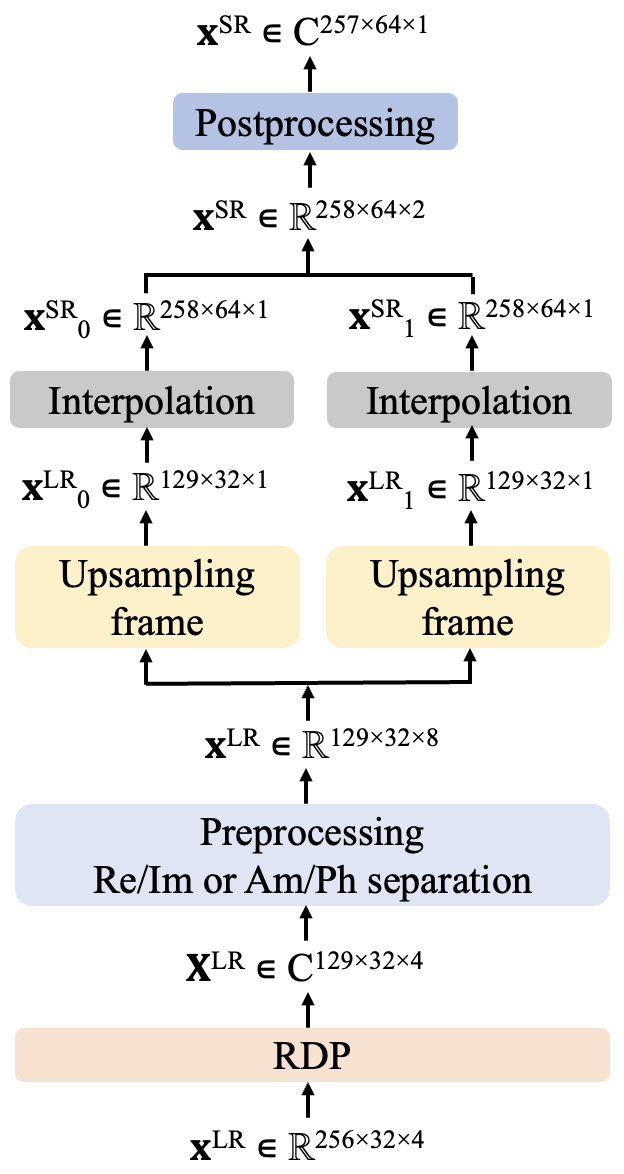
\includegraphics[height=1.07\textwidth]{MA_presentation/figures/interpolation_left.png}
            % \caption{Low-resolution with the factor 2}
        \end{minipage}
        % \hspace{0.3cm}
        \begin{minipage}{0.39\textwidth}
            \centering
            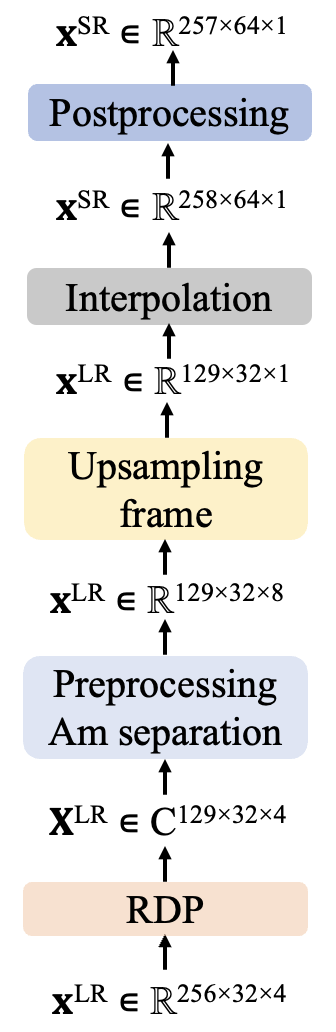
\includegraphics[height=1.6\textwidth]{MA_presentation/figures/interpolation_right.png}
            % \caption{High-resolution}
        \end{minipage}
        \caption{Interpolation model according to the input data representation}
    \end{figure}

\end{frame}



\begin{frame}[t]{CNN model}
    \begin{itemize}
        \item Convolutional neural network (CNN) model
    \end{itemize}
    \begin{figure}
        \centering
        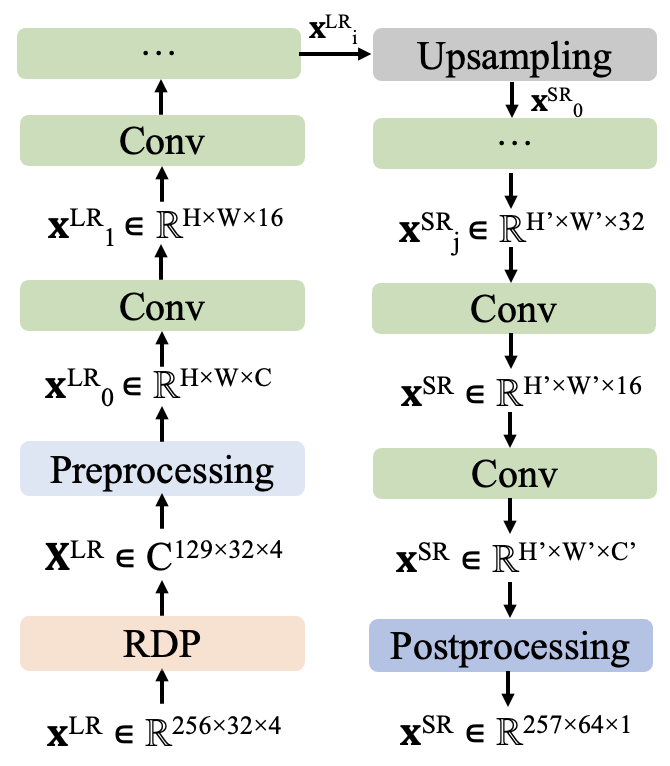
\includegraphics[scale=.46]{MA_presentation/figures/cnn_simple.png}
        \caption{CNN model}
    \end{figure}

\end{frame}


\begin{frame}[t]{UNet model}

    \begin{figure}
        \centering
        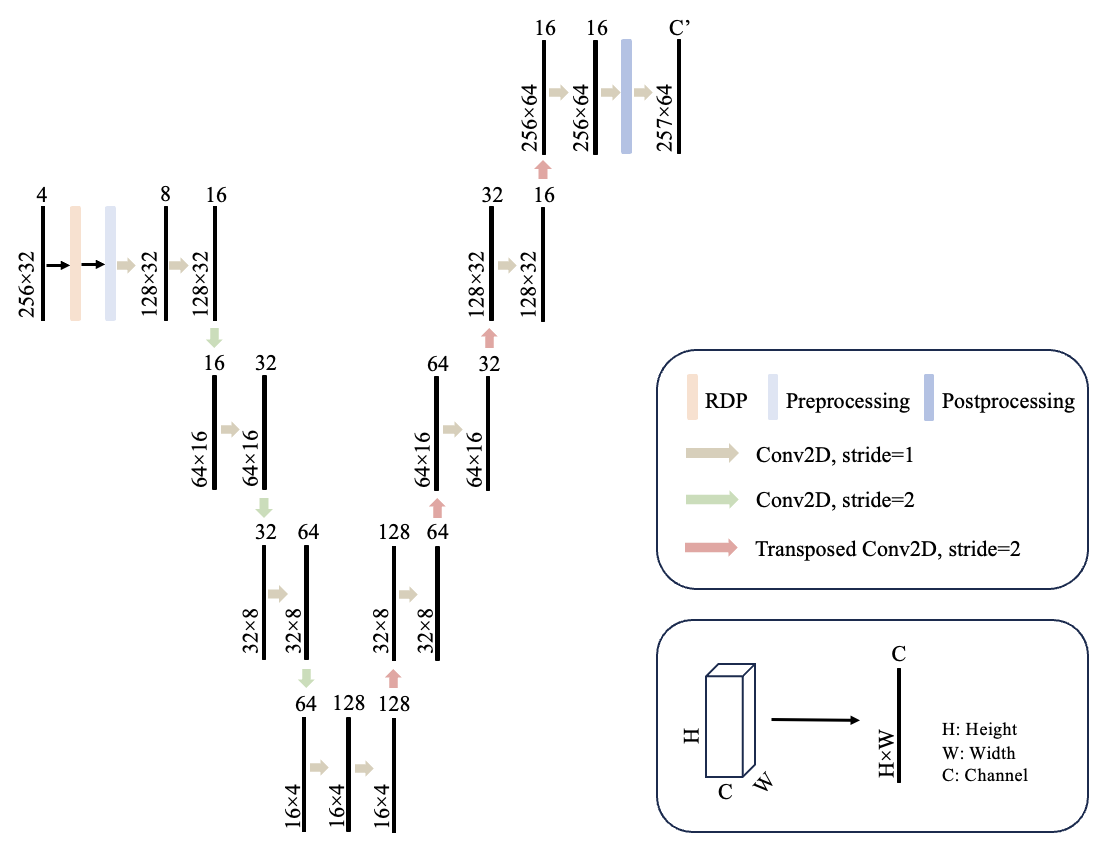
\includegraphics[scale=.46]{MA_presentation/figures/unet_model.png}
        \caption{UNet model}
    \end{figure}

\end{frame}



\begin{frame}[t]{UNet concat model \cite{prabhakara_high_2023}}

    \begin{figure}
        \centering
        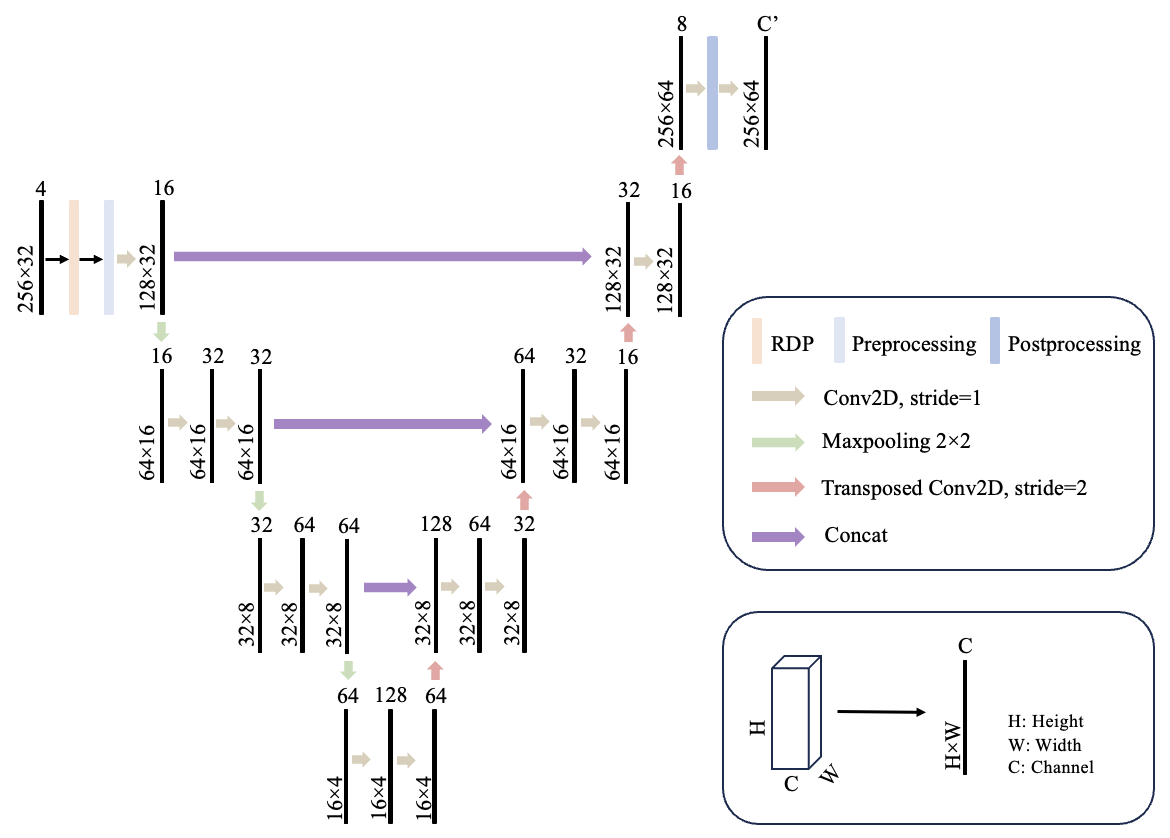
\includegraphics[scale=.45]{MA_presentation/figures/unet_concat.png}
        \caption{UNet concat model, adapted from \cite{prabhakara_high_2023}}
    \end{figure}

\end{frame}


\begin{frame}[t]{DP-TF Transformer model}
    \begin{itemize}
        \item Dual-Path Time-Frequency (DP-TF) Transformer model \cite{hinderer_blind_2022}
    \end{itemize}

    % \hspace{0.2cm}
    
    \begin{figure}
        \centering
        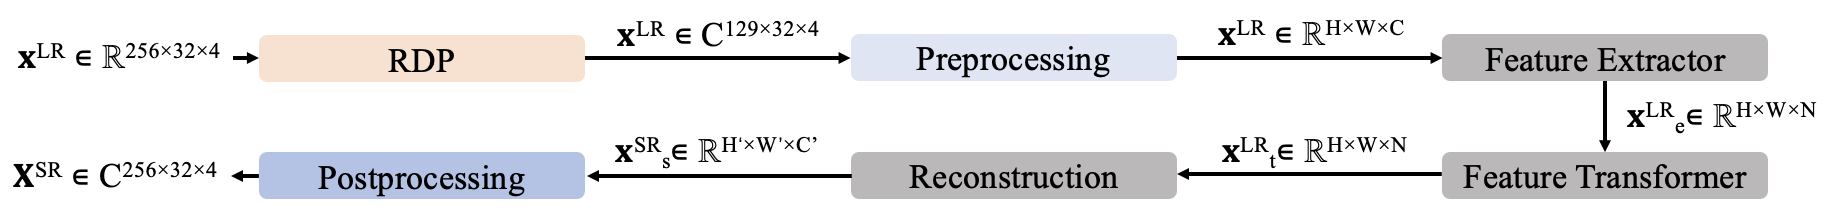
\includegraphics[scale=.35]{MA_presentation/figures/dp-tf_transformer_architecture.png}
        \caption{DP-TF Transformer model, adapted from \cite{hinderer_blind_2022}}
    \end{figure}

    \hspace{0.2cm}

    \begin{figure}
        \centering
        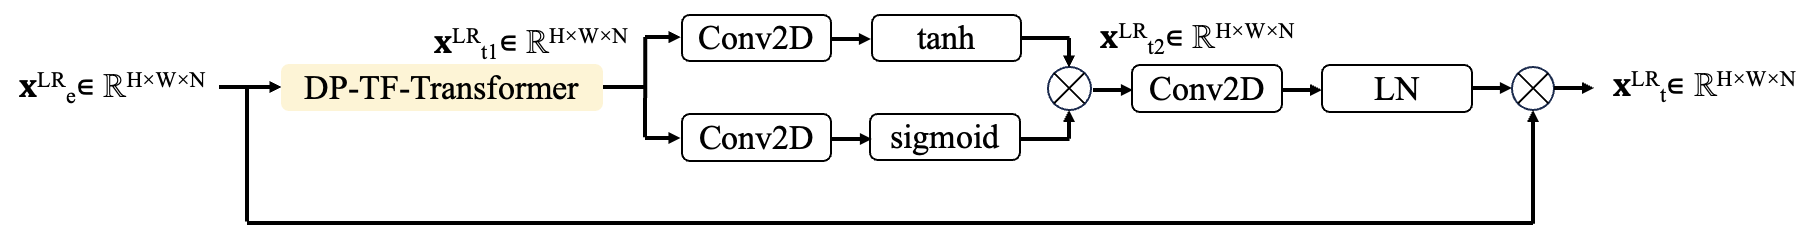
\includegraphics[scale=.35]{MA_presentation/figures/feature_transformer_block.png}
        \caption{Feature Transformer block, adapted from \cite{hinderer_blind_2022}}
    \end{figure}

\end{frame}


\begin{frame}[t]{DP-TF Transformer model}

    \hspace{0.2cm}
    
    \begin{figure}
        \centering
        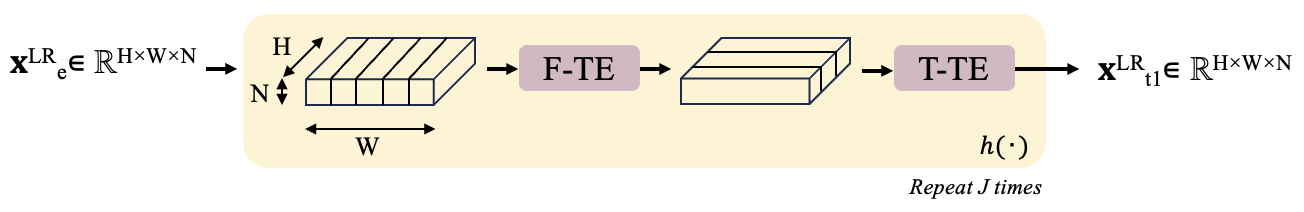
\includegraphics[scale=.47]{MA_presentation/figures/dp_transformer_block.png}
        \caption{DP-TF-Transformer block, adapted from \cite{hinderer_blind_2022}}
        \label{dp-tf transformer block}
    \end{figure}

    % \hspace{0.2cm}

    \begin{figure}
        \centering
        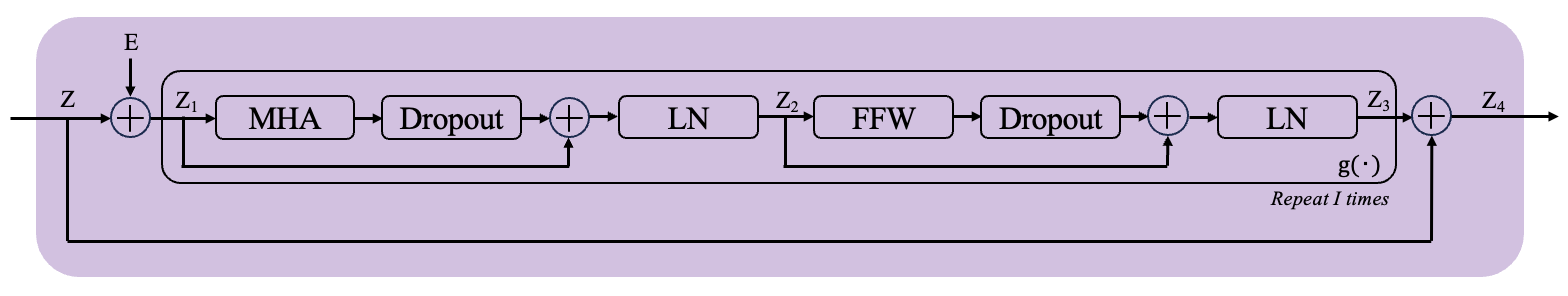
\includegraphics[scale=.38]{MA_presentation/figures/transformer_block.png}
        \caption{Transformer encoder (TE) block, adapted from \cite{hinderer_blind_2022}}
    \end{figure}

\end{frame}


\begin{frame}[t]{SwinIR Transformer architecture}
    \begin{itemize}
        \item Image restoration with Swin Transformer (SwinIR) architecture \cite{liang_swinir_2021}
    \end{itemize}
    
    \begin{figure}
        \hspace{-0.2cm}
        \centering
        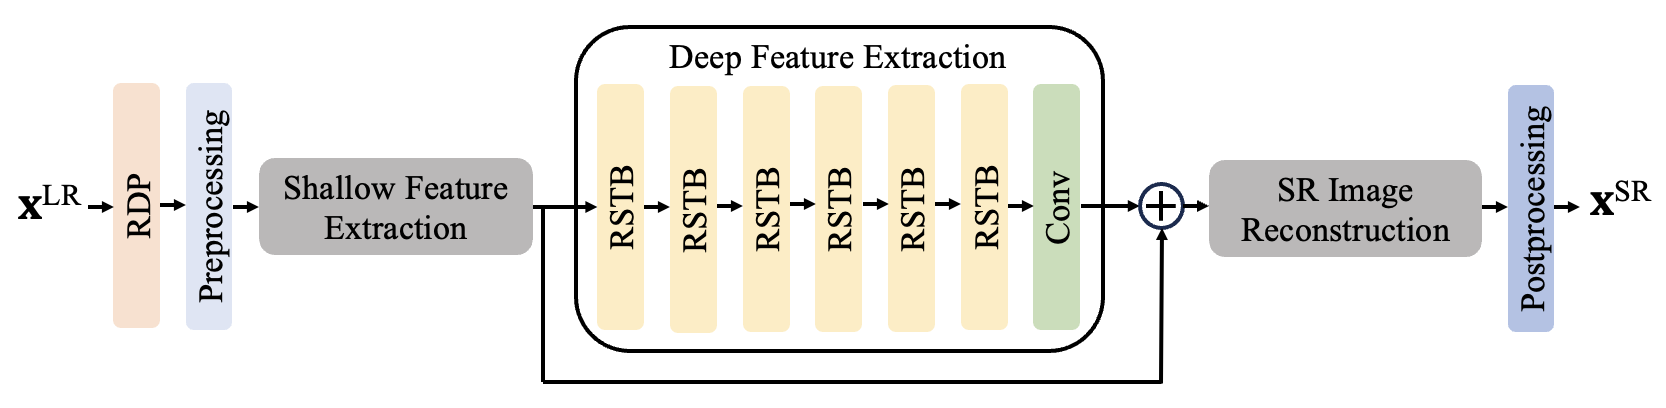
\includegraphics[scale=.38]{MA_presentation/figures/swinir_architecture.png}
        \caption{SwinIR Transformer architecture, adapted from \cite{liang_swinir_2021}}
    \end{figure}

    % \hspace{0.1cm}

    \begin{figure}
        \centering
        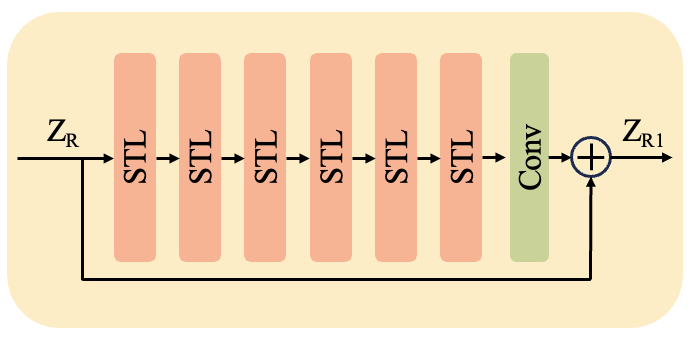
\includegraphics[scale=.42]{MA_presentation/figures/rstb_block.png}
        \caption{Residual Swin Transformer blocks (RSTB), adapted from \cite{liang_swinir_2021}}
    \end{figure}

\end{frame}


\begin{frame}[t]{SwinIR Transformer models}
    
    \begin{figure}
        \centering
        \hspace{-0.2cm}
        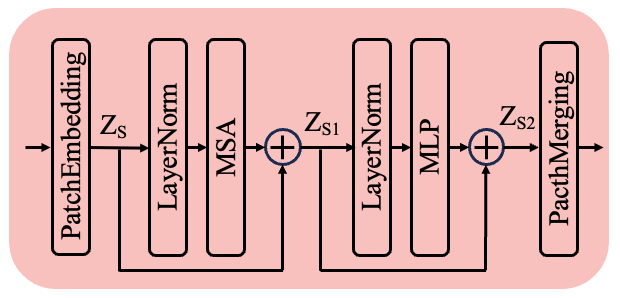
\includegraphics[scale=.55]{MA_presentation/figures/stl_block.png}
        \caption{SwinIR+Swin: Swin Transformer layers (STL) block, adapted from \cite{liang_swinir_2021}}
    \end{figure}

    % \hspace{0.1cm}

    \begin{figure}
        \centering
        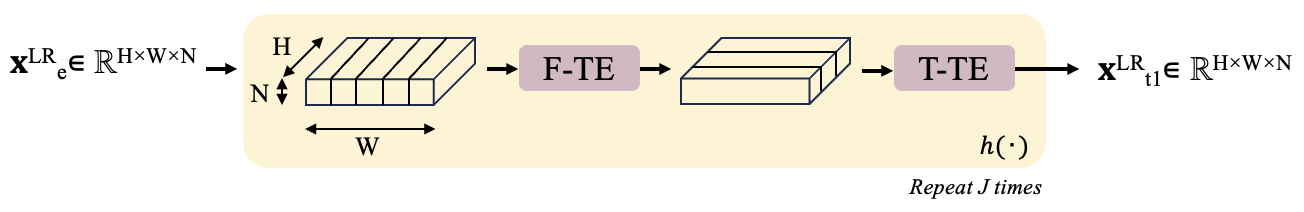
\includegraphics[scale=.47]{MA_presentation/figures/dp_transformer_block.png}
        \caption{SwinIR+DP: DP-TF Transformer block, adapted from \cite{hinderer_blind_2022}}
    \end{figure}

\end{frame}


\begin{frame}[t]{cGAN model}
    
    \begin{itemize}
        \item Conditional generative adversarial network (cGAN) model \cite{team_keras_cgan}
        \item Generator
        \hspace{0.1cm}
        \item Discriminator
    \end{itemize}

    % \hspace{0.1cm}

    \begin{figure}
        \centering
        \begin{minipage}{0.49\textwidth}
            \centering
            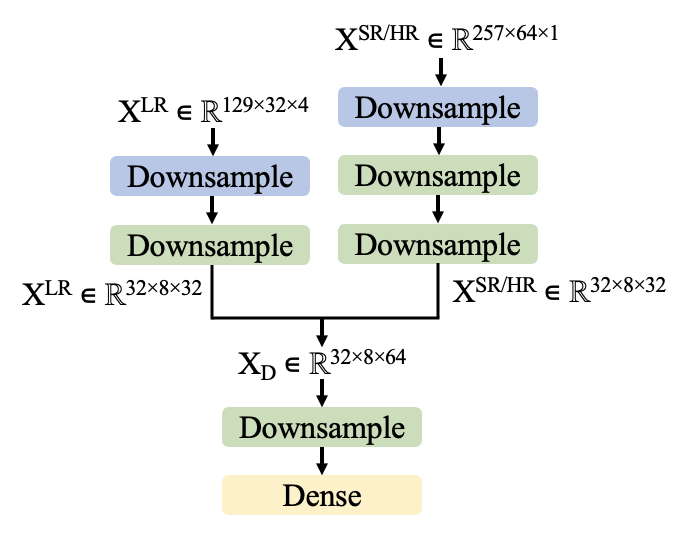
\includegraphics[height=1.0\textwidth]{MA_presentation/figures/discriminator_left.png}
            % \caption{Low-resolution with the factor 2}
        \end{minipage}
        % \hspace{0.3cm}
        \begin{minipage}{0.49\textwidth}
            \centering
            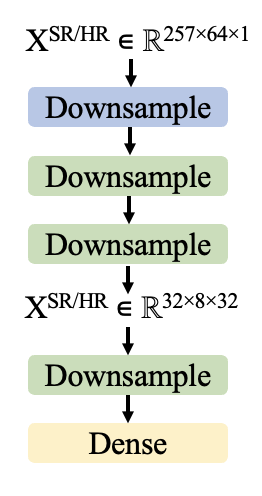
\includegraphics[height=1.0\textwidth]{MA_presentation/figures/discriminator_right.png}
            % \caption{High-resolution}
        \end{minipage}
        \caption{Discriminator models with and without low-resolution inputs}
    \end{figure}

\end{frame}




%% ===================================================================
\section{Loss functions}
\setcounter{section}{3}
\setcounter{figure}{0}
% --------------------------------------------------------------------

% \begin{frame}[t]{Loss functions}
    
%     \begin{itemize}
%         \item Mean squared error (MSE)
%         \vspace{0.5\baselineskip}
%         \item Weighted MSE (WMSE)
%         \vspace{0.5\baselineskip}
%         \item Signal-to-distortion ratio (SDR) \cite{roux_sdr_2018}
%         \vspace{0.5\baselineskip}
%         \item Logarithmic spectral distance (LSD) \cite{braun_consolidated_2020}
%         \vspace{0.5\baselineskip}
%         \item Phase-aware logarithmic spectral distance (PLSD) \cite{braun_consolidated_2020}
%         \vspace{0.5\baselineskip}
%         \item Very Deep Convolutional Networks (VGG) perceptual loss \cite{johnson_perceptual_2016}
%         \vspace{0.5\baselineskip}
%         \item Loss combination
%         \vspace{0.5\baselineskip}
%         \item Adversarial loss
%             \begin{itemize}
%                 \vspace{0.3\baselineskip}
%                 \item Generator loss
%                 \vspace{0.3\baselineskip}
%                 \item Discriminator loss
%             \end{itemize}
%     \end{itemize}

% \end{frame}



\begin{frame}[t]{Loss functions}
    \begin{itemize}
        \item Mean squared error (MSE)
        \begin{equation}
            \centering
            \mathcal{L}_{\text{MSE}} = \frac{1}{n} \sum_{i=1}^{n} (Y_i - \hat{Y}_i)^2
        \end{equation}

        \vspace{0.3\baselineskip}
    
        \begin{equation}
            \centering
            \mathcal{L}_{\text{MSE}} = \mathcal{L}_{\text{MSE, Re/Amp}} + \lambda \times \mathcal{L}_{\text{MSE, Im/Ph}}
        \end{equation}

        \vspace{1.5\baselineskip}
        
        \item Weighted MSE (WMSE)
        \begin{equation}
            \centering
            \mathcal{L}_{\text{WMSE, Amp}} = \frac{1}{n} \sum_{i=1}^{n} \frac{(A_i - \hat{A}_i)^2}{A_i}
            \label{amplitude wmse loss equation}
        \end{equation}

        \vspace{0.3\baselineskip}
        
        \begin{equation}
            \centering
            \mathcal{L}_{\text{WMSE}} = \mathcal{L}_{\text{WMSE, Amp}} + \lambda \times \mathcal{L}_{\text{MSE, Ph}}
        \end{equation}
    \end{itemize}
    
    
\end{frame}


\begin{frame}[t]{Loss functions}

    \begin{itemize}
        \item Signal-to-distortion ratio (SDR) \cite{roux_sdr_2018}
            \begin{equation}
                \centering
                \mathcal{L}_{\text{SDR}} = 10 \log_{10} \left( \frac{\|A\|^2}{\|A - \hat{A}\|^2} \right)
                \label{sdr equation}
            \end{equation}

        \vspace{1.5\baselineskip}
        
        \item Logarithmic spectral distance (LSD) \cite{braun_consolidated_2020}
            \begin{equation}
                \centering
                \mathcal{L}_{\text{LSD, Amp}} = \left\{ \frac{1}{N} \sum_{n=1}^{N} \left[ \log_{10} A(n) - \log_{10} \hat{A}(n) \right]^2 \right\}^{\frac{1}{2}}
                \label{final lsd equation}
            \end{equation}

            \vspace{0.3\baselineskip}

            \begin{equation}
                \centering
                \mathcal{L}_{\text{LSD}} = \mathcal{L}_{\text{LSD, Amp}} + \lambda \times \mathcal{L}_{\text{MSE, Ph}}
            \end{equation}
    \end{itemize}
    
\end{frame}


\begin{frame}{Mask in LSD loss}
    \begin{figure}
        \centering

        % Top row: two images side by side
        \begin{minipage}{0.48\textwidth}
            \centering
            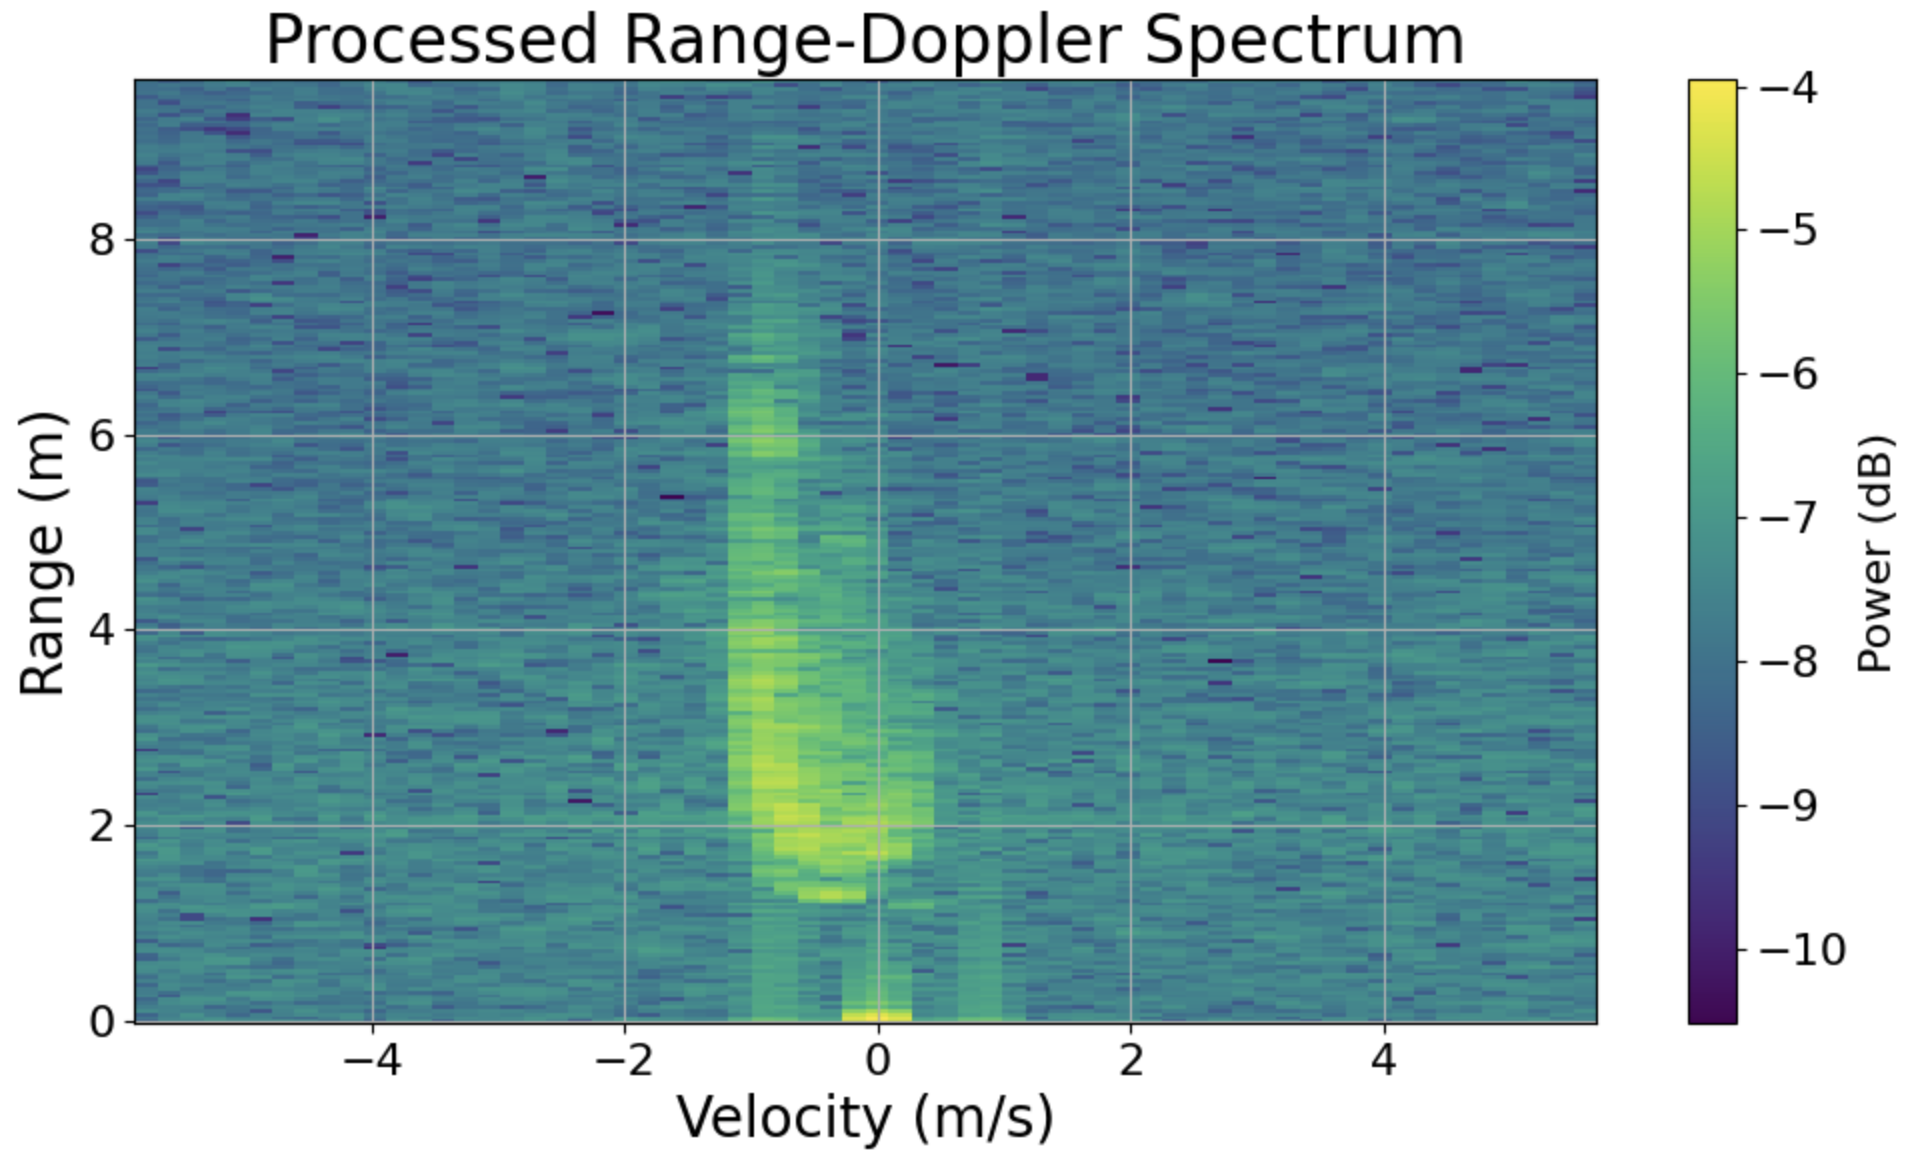
\includegraphics[width=\textwidth]{MA_presentation/figures/gt_logamp.png}
            % \small High-resolution with log amplitude
        \end{minipage}
        \hfill
        \begin{minipage}{0.48\textwidth}
            \centering
            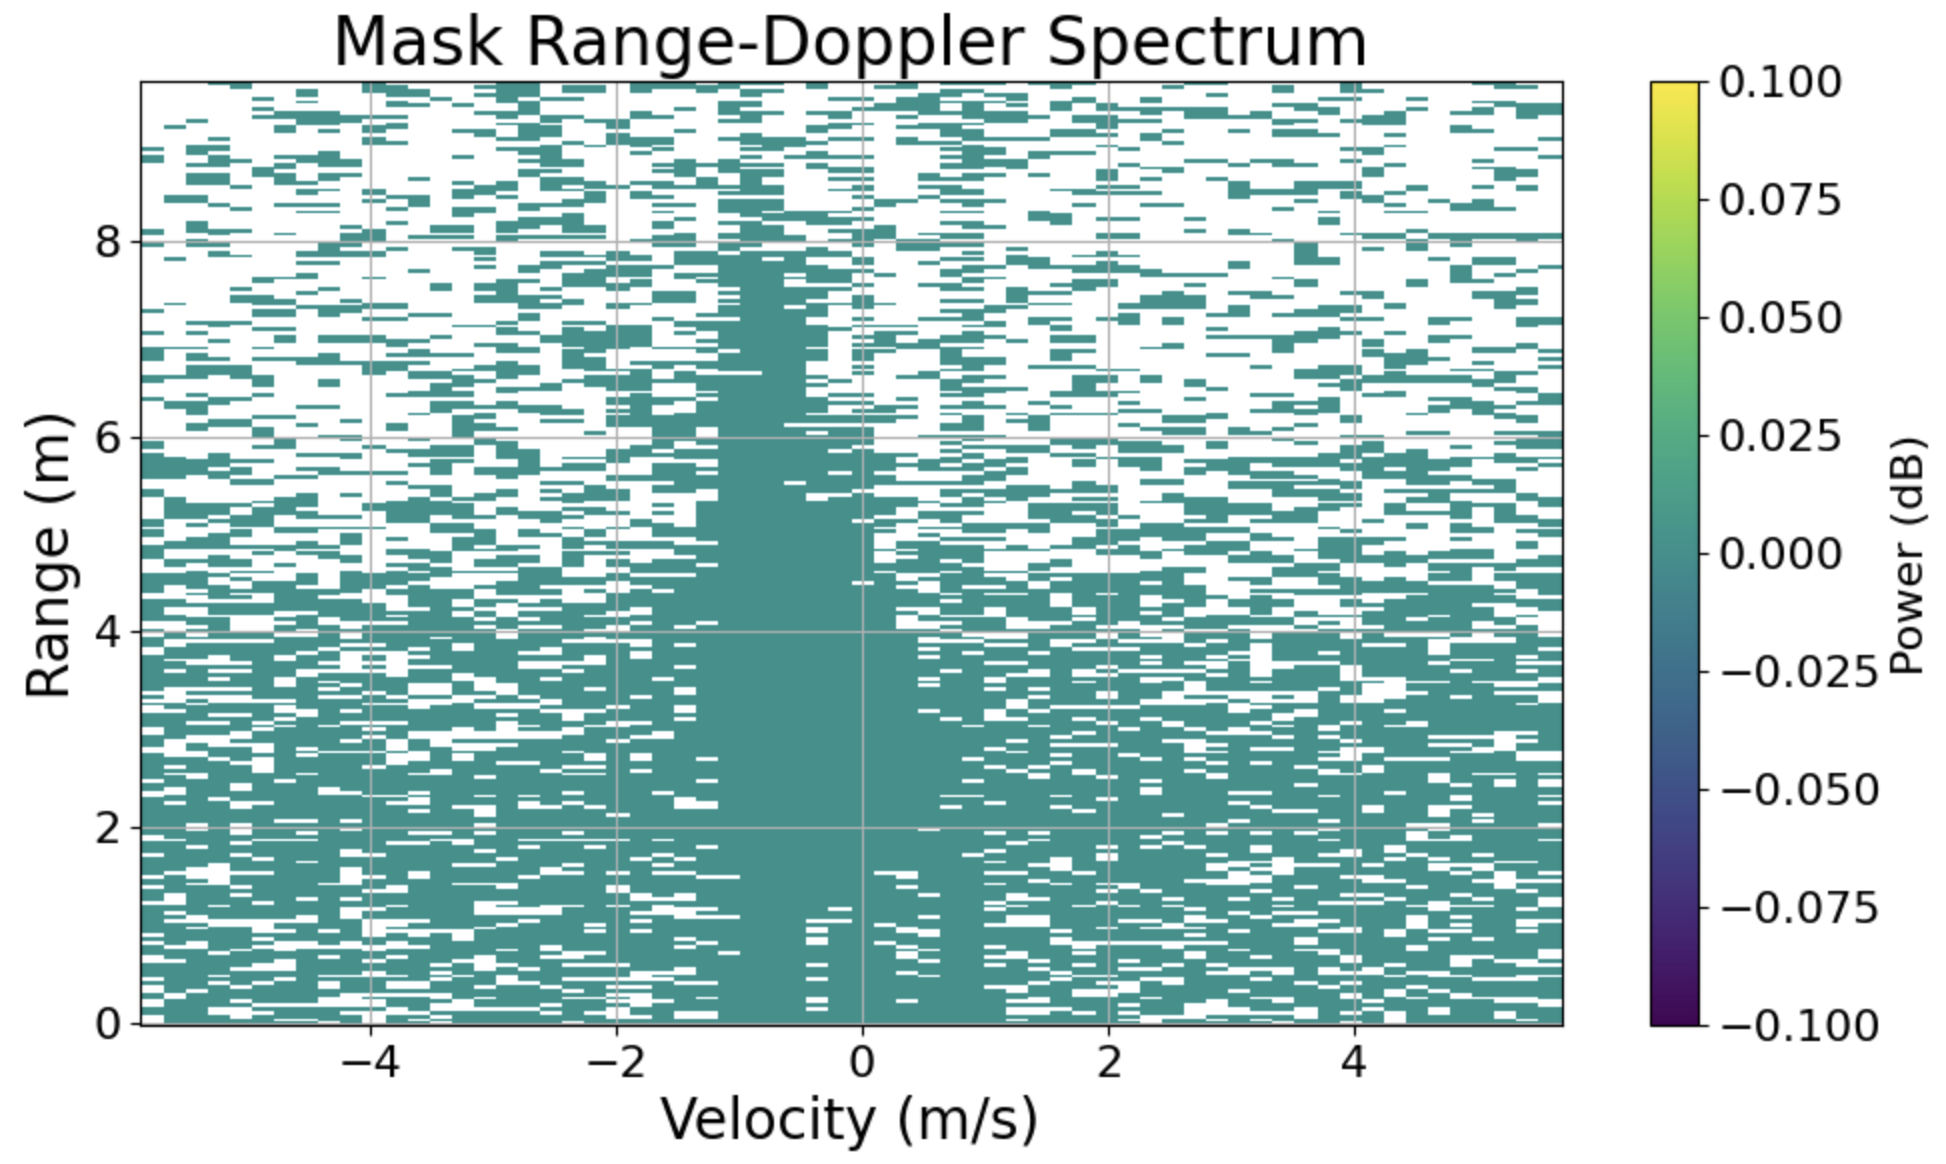
\includegraphics[width=\textwidth]{MA_presentation/figures/mask.png}
            % \small Mask
        \end{minipage}

        \vspace{0.1cm}

        % Bottom image centered
        \begin{minipage}{0.5\textwidth}
            \centering
            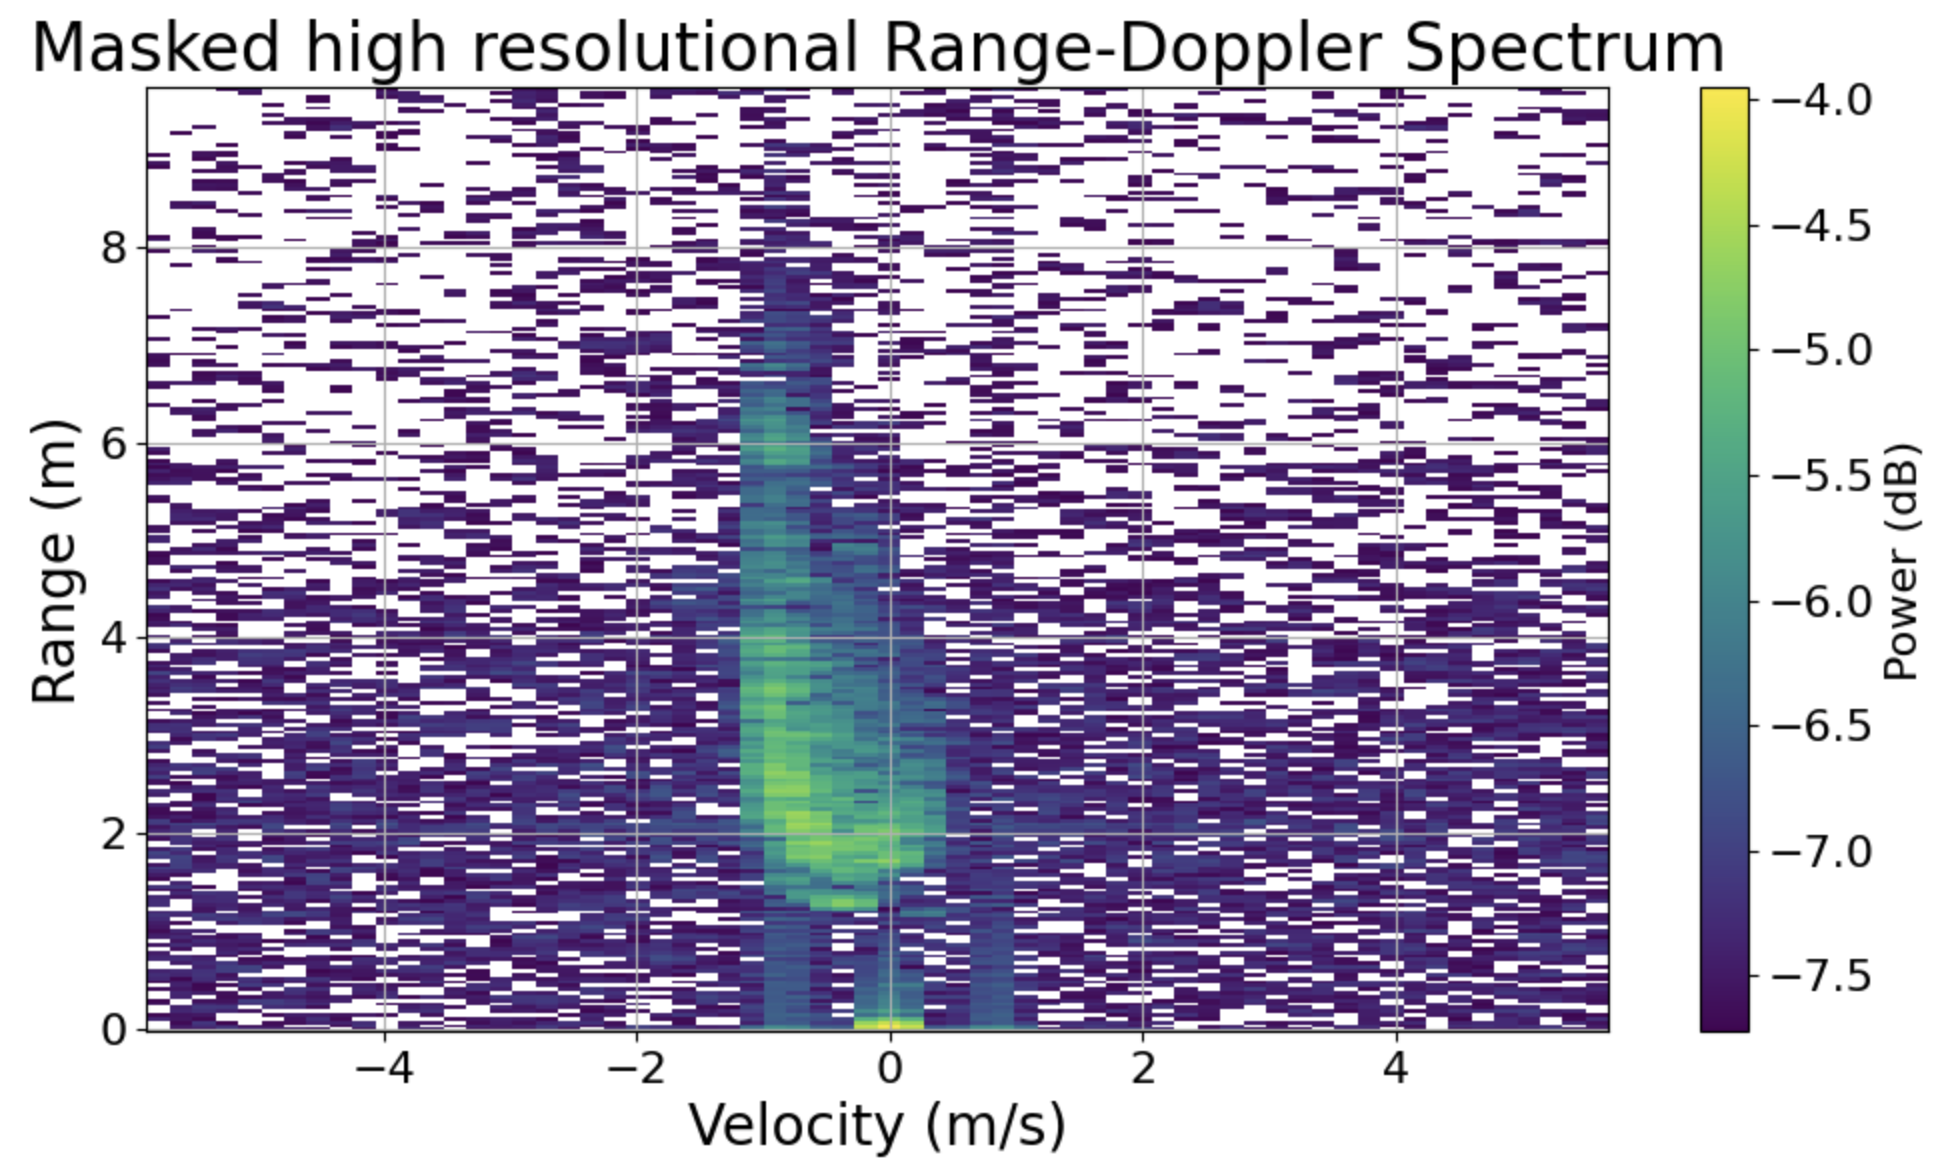
\includegraphics[width=\textwidth]{MA_presentation/figures/masked_gt.png}
            % \small Masked high-resolution image
        \end{minipage}

        \caption{Mask in LSD loss function. From left to right: processed high-resolution data, mask; below: masked data.}
    \end{figure}
\end{frame}




\begin{frame}[t]{Loss functions}

    \begin{itemize}
        \vspace{1.0\baselineskip}
        
        \item Phase-aware logarithmic spectral distance (PLSD) \cite{braun_consolidated_2020}
            \begin{equation}
                \centering
                \mathcal{L}_{\text{PLSD}} = \left\langle \left| \log_{10} \left| \frac{\hat{Y}}{Y} \right| \right| \times \left( 2 - \cos{(\varphi_{\hat{Y}} - \varphi_{Y})} \right) \right\rangle
            \end{equation}

        \vspace{1.8\baselineskip}
        
        \item VGG perceptual loss \cite{johnson_perceptual_2016}
            \begin{equation}
                \centering
                \mathcal{L}_{\text{Perceptual}} (\hat{Y}, Y) = \frac{1}{H W C} \left\| \phi (\hat{Y}) - \phi (Y) \right\|_2^2
            \end{equation}
    \end{itemize}
    
\end{frame}



\begin{frame}[t]{Loss functions}

    \begin{itemize}
        \item Loss combination, such as
            \begin{equation}
                \centering
                \mathcal{L}_{\text{Combination}} = \mathcal{L}_{\text{LSD}} + \lambda_c \times \mathcal{L}_{\text{Perceptual}}
                \label{loss combination equation}
            \end{equation}

        \vspace{0.5\baselineskip}
        
        \item Adversarial loss
        \vspace{0.5\baselineskip}

        \begin{itemize}
            \item Generator loss
            \vspace{0.3\baselineskip}
                \begin{equation}
                    \centering
                    \mathcal{L}_{\text{Gen}} = \mathcal{L}_{\text{Combination}} + \lambda_g \times \| 1 - P_{\text{Super}} \|_{2}
                \end{equation}
                
            \vspace{0.3\baselineskip}
            
            \item Discriminator loss
            \vspace{0.3\baselineskip}
                \begin{equation}
                    \centering
                    \mathcal{L}_{\text{Disc}} = \| 1 - P_{\text{High}} \|_{2} + \| 0 - P_{\text{Super}} \|_{2}
                \end{equation}
            
        \end{itemize}
            
    \end{itemize}
    
\end{frame}


%% ===================================================================
\section{Evaluation}
\setcounter{section}{4}
\setcounter{figure}{0}
\setcounter{table}{0}
% --------------------------------------------------------------------

\begin{frame}{Evaluation}
    \vspace{-1.0\baselineskip}
    \begin{itemize}
        \item Evaluation one by one
        \vspace{0.5\baselineskip}
        \item Only amplitude loss in the evaluation of loss functions
        \vspace{0.5\baselineskip}
        \item Convert back the logarithm and normalization
        \vspace{0.5\baselineskip}
        \item Small model and data subset
        \vspace{0.5\baselineskip}
        \item Criteria: Lower evaluation loss and better visual effect
    \end{itemize}
\end{frame}

\begin{frame}[t]{Models evaluation}

    \begin{table}
        \centering
        \vspace{0.5\baselineskip}
        \small
        \caption{Evaluation losses of different models in the case of the MSE and common processing methods.}
        \label{models comparison in the case of the MSE and original processing methods}
        \vspace{-0.5cm}
        \begin{tabular}{l|c|c|c|c|c|c}
            \hline
            Models & \#Params & MSE & SDR & LSD & WMSE & Perceptual \\
            \hline
            Interpolation & 0 & 3.570 & -3.620 & 0.750 & 0.774 & 28.010 \\
            \hline
            CNN & 103,684 & 2.164 & -5.028 & \textbf{0.441} & 3.599 & 25.133 \\
            \hline
            UNet & 93,162 & 1.352 & -2.872 & 0.600 & 1.034 & 22.014 \\
            \hline
            UNet concat & 96,746 & \textbf{1.275} & -3.609 & 0.552 & 0.968 & \textbf{21.847} \\
            \hline
            DP & 113,964 & 3.212 & -4.926 & 0.611 & \textbf{0.163} & 23.583 \\
            \hline
            SwinIR+DP & 97,252 & 1.754 & \textbf{-5.787} & 0.503 & 0.314 & 22.764 \\
            \hline
            SwinIR+Swin & 111,624 & 1.541 & -4.505 & 0.546 & 1.104 & 26.381 \\
            \hline
        \end{tabular}
    \end{table}
    
\end{frame}


\begin{frame}{Models evaluation}
    \begin{figure}
        \centering
        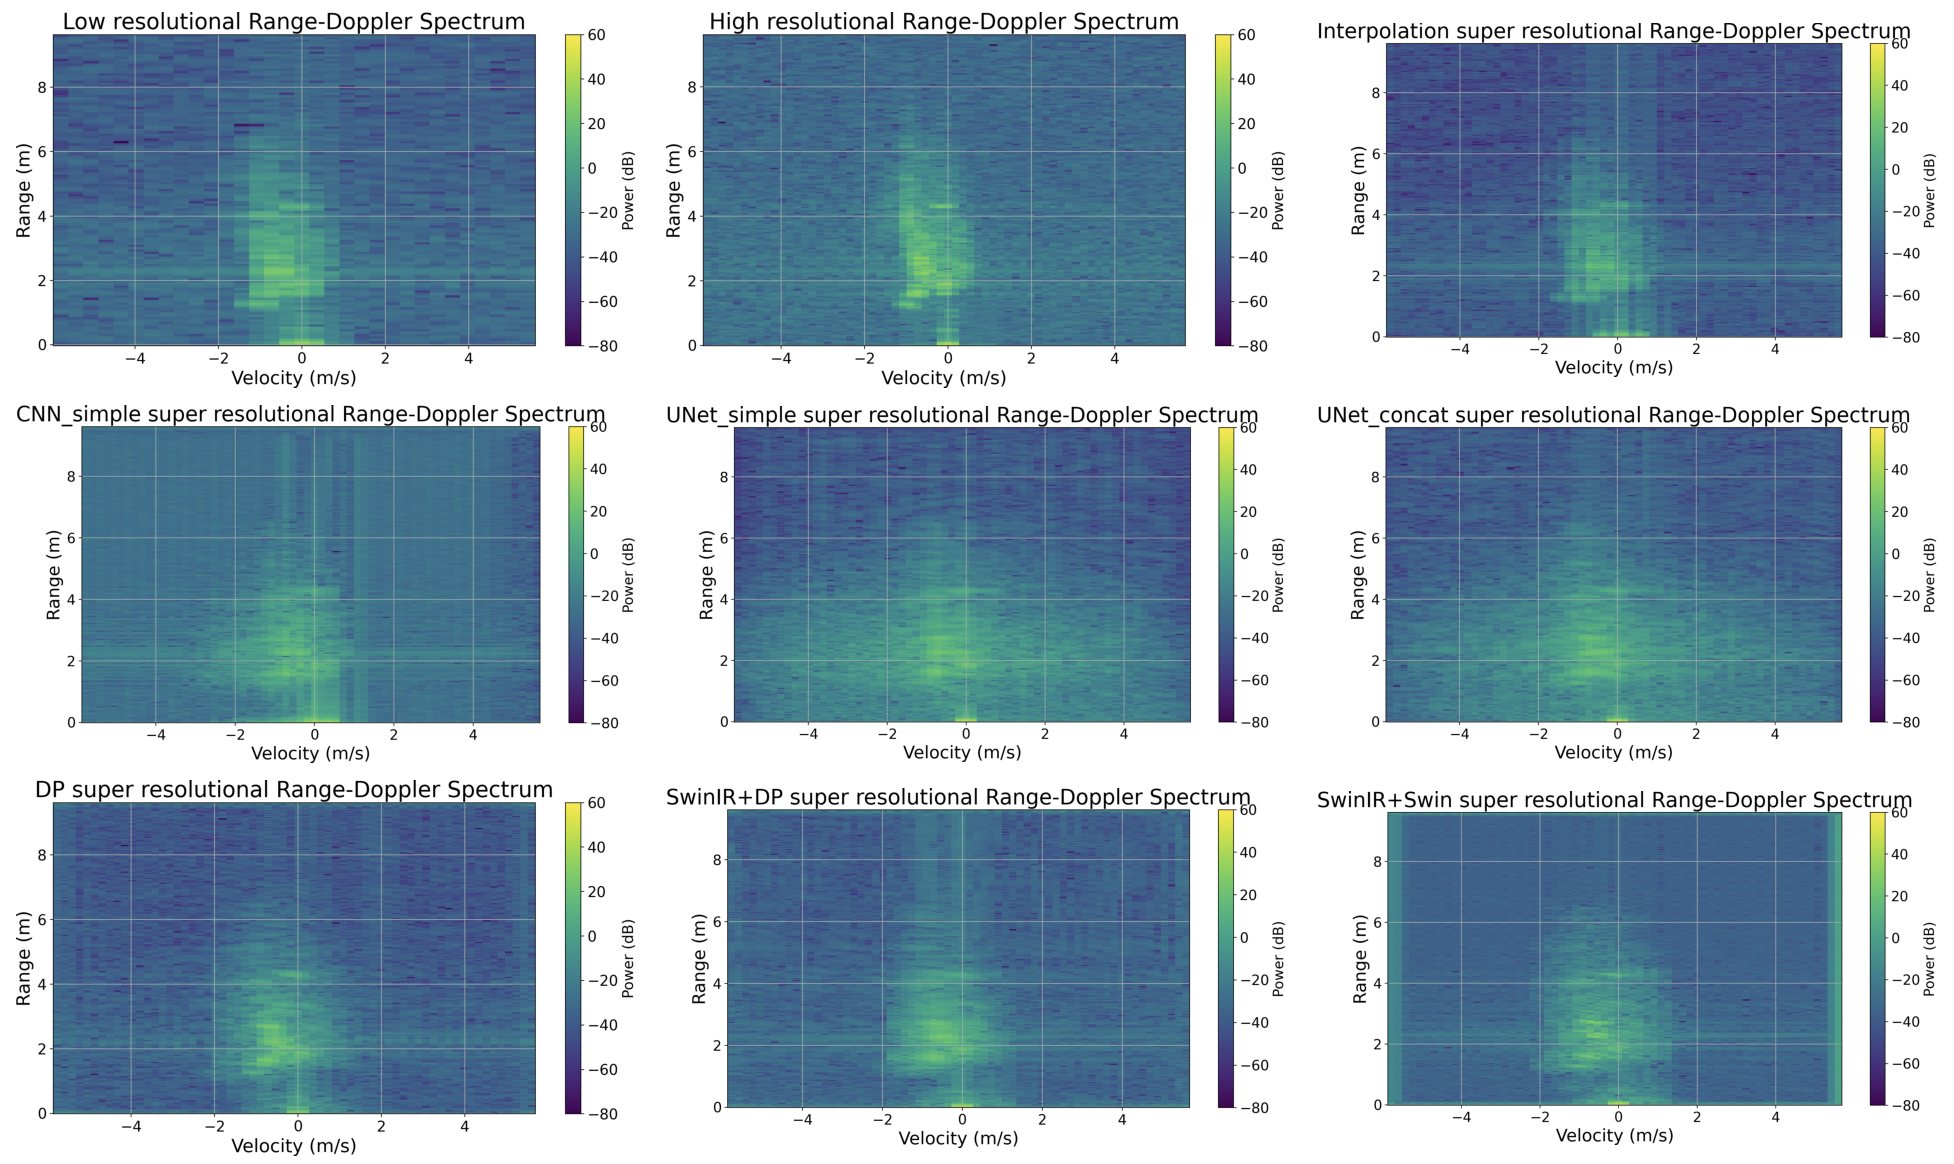
\includegraphics[scale=.3]{MA_presentation/figures/evaluation_models_1.png}
        \vspace{-0.18cm}
        \caption{Range-Doppler maps in the case of MSE and common processing methods, from left to right, first row: low-resolution, high-resolution, interpolation; the second row: CNN, UNet, UNet concat; third row: DP, SwinIR+DP, SwinIR+Swin.}
        \label{evaluation models 1}
    \end{figure}
\end{frame}


% \begin{frame}{Evaluation}
%     \begin{itemize}
%         \item Processing methods
%         \vspace{0.5\baselineskip}
%         \begin{itemize}
%             \item Input data representation
%             \vspace{0.3\baselineskip}
%             \item Dimension processing types
%             \vspace{0.3\baselineskip}
%             \item Upsampling types
%             \vspace{0.3\baselineskip}
%             \item Logarithm types
%             \vspace{0.3\baselineskip}
%             \item Amplitude normalization types
%             \vspace{0.3\baselineskip}
%             \item Angle normalization types
%         \end{itemize}
%     \end{itemize}
% \end{frame}


\begin{frame}{Processing methods evaluation}

    \begin{table}
        \centering
        \small
        \caption{Evaluation losses of different input data representations}
        % \vspace{-2.5ex} 
        \label{Evaluation losses of the separation types comparison}
        \vspace{-0.2cm}
        \begin{tabular}{l|c|c|c|c|c}
            \hline
            Representation types & MSE & SDR & LSD & WMSE & Perceptual \\
            \hline
            Real/Imaginary & 3.435 & -4.958 & 0.619 & \textbf{0.155} & 24.682 \\
            \hline
            Amplitude & \textbf{3.136} & \textbf{-7.778} & \textbf{0.385} & 0.181 & \textbf{18.101} \\
            \hline
            Amplitude/Phase & 3.213 & -5.068 & 0.493 & 0.241 & 20.126 \\
            \hline
        \end{tabular}
    \end{table}

    \vspace{-0.2\baselineskip}

    \begin{table}
        \centering
        \small
        \caption{Evaluation losses of different dimension processing types}
        \label{Evaluation losses of the dimension processing types comparison}
        \vspace{-0.2cm}
        \begin{tabular}{l|c|c|c|c|c}
            \hline
            Dimension & MSE & SDR & LSD & WMSE & Perceptual \\
            \hline
            No processing & 3.100 & -6.312 & 0.427 & 0.194 & 19.081 \\
            \hline
            Padding & 3.113 & \textbf{-6.611} & \textbf{0.420} & \textbf{0.190} & 19.092 \\
            \hline
            Convolution & \textbf{2.349} & -5.908 & 0.451 & 0.206 & \textbf{16.259} \\
            \hline
        \end{tabular}
    \end{table}

    \vspace{-0.2\baselineskip}

    \begin{table}
        \centering
        \hspace{-1.0cm}
        \small
        \caption{Evaluation losses of different upsampling types}
        \label{Evaluation losses of the upsampling types comparison}
        \vspace{-0.25cm}
        \begin{tabular}{l|c|c|c|c|c|c}
            \hline
            Upsampling & \#Params & MSE & SDR & LSD & WMSE & Perceptual \\
            \hline
            Transposed & 113,866 & 3.113 & \textbf{-6.611} & \textbf{0.420} & \textbf{0.190} & 19.092 \\
            \hline
            Pixel shuffle & 48,042 & \textbf{2.560} & -4.206 & 0.506 & 0.269 & \textbf{17.918} \\
            \hline
        \end{tabular}
    \end{table}

\end{frame}


% \begin{frame}{Dimension processing types evaluation}
%     \begin{table}
%         \centering
%         % \scriptsize
%         \caption{Evaluation losses of different dimension processing types}
%         \label{Evaluation losses of the dimension processing types comparison}
%         \begin{tabular}{l|c|c|c|c|c}
%             \hline
%             Dimension & MSE & SDR & LSD & WMSE & Perceptual \\
%             \hline
%             No processing & 3.100 & -6.312 & 0.427 & 0.194 & 19.081 \\
%             \hline
%             Padding & 3.113 & \textbf{-6.611} & \textbf{0.420} & \textbf{0.190} & 19.092 \\
%             \hline
%             Convolution & \textbf{2.349} & -5.908 & 0.451 & 0.206 & \textbf{16.259} \\
%             \hline
%         \end{tabular}
%     \end{table}

%     \begin{figure}
%         \centering
%         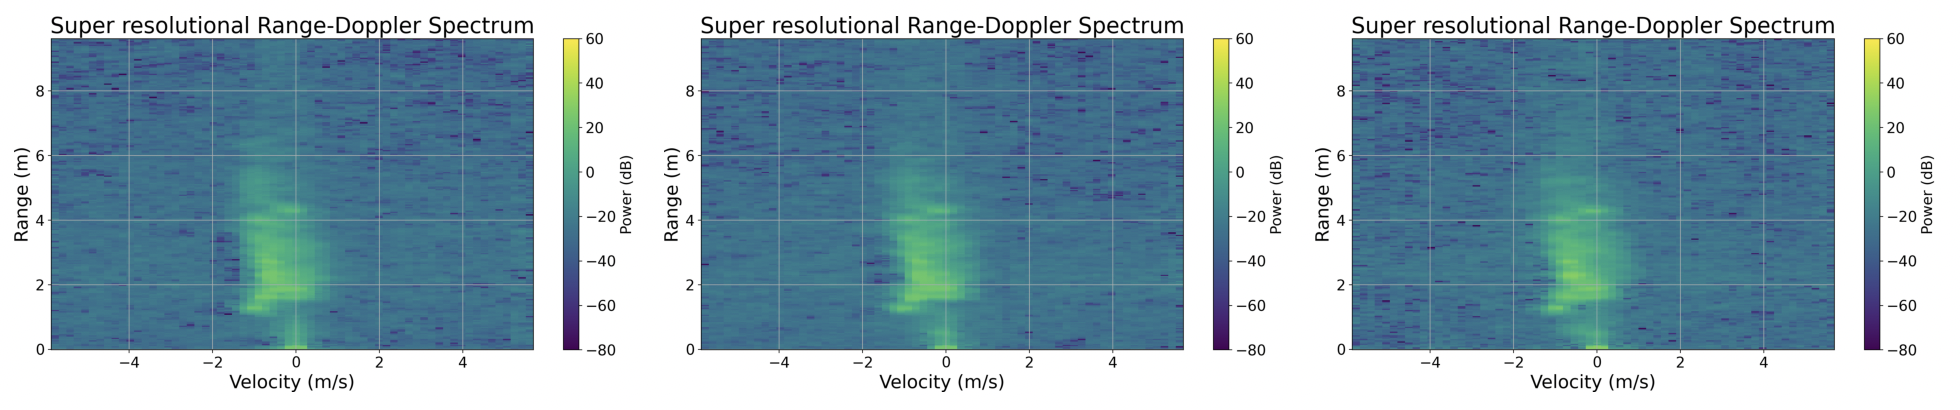
\includegraphics[scale=.34]{MA_presentation/figures/evaluation_processing_mse_B.png}
%         \caption{Super-resolution images of different dimension processing types, from left to right no processing, padding and convolutional layer, respectively.}
%         \label{super-resolution images of the dimension processing types}
%     \end{figure}
% \end{frame}

    
% \begin{frame}{Upsampling types evaluation}
%     \begin{table}
%         \centering
%         \scriptsize
%         \caption{Evaluation losses of different upsampling types, where C1 represents the transposed convolutional layer and C2 denotes the pixel shuffle approach as the upsampling layer.}
%         \label{Evaluation losses of the upsampling types comparison}
%         \begin{tabular}{l|c|c|c|c|c|c}
%             \hline
%             Upsampling types & \#Params & MSE & SDR & LSD & WMSE & Perceptual \\
%             \hline
%             C1 & 113,866 & 3.113 & \textbf{-6.611} & \textbf{0.420} & \textbf{0.190} & 19.092 \\
%             \hline
%             C2 & 48,042 & \textbf{2.560} & -4.206 & 0.506 & 0.269 & \textbf{17.918} \\
%             \hline
%         \end{tabular}
%     \end{table}

%     \begin{figure}
%         \centering
%         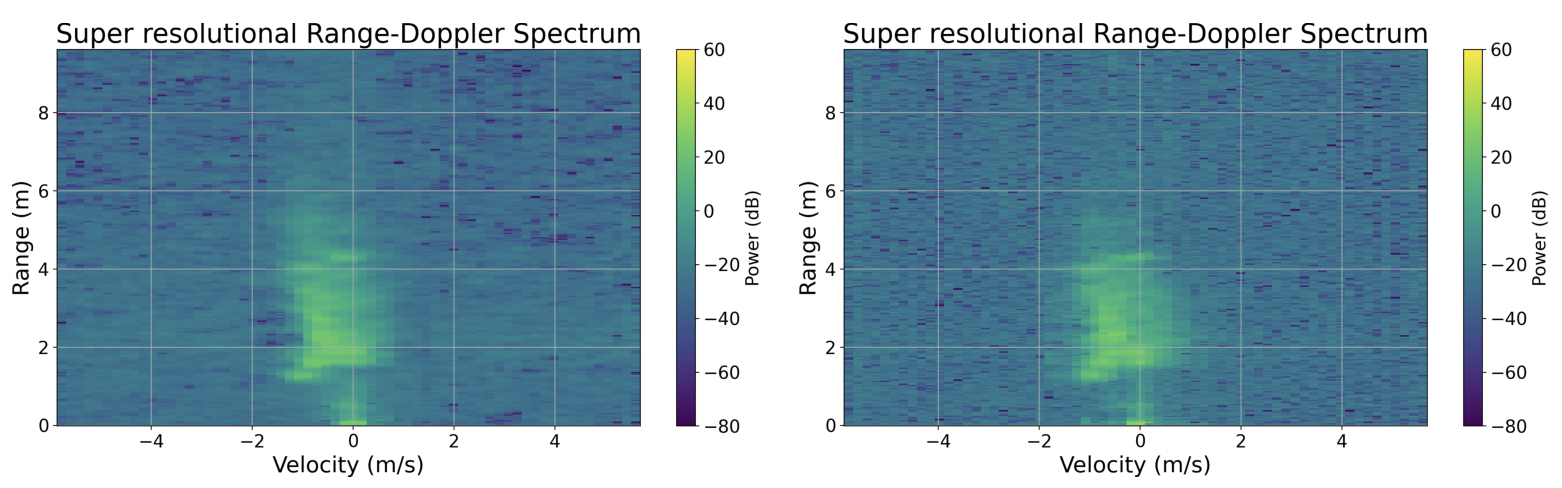
\includegraphics[scale=.34]{MA_presentation/figures/evaluation_processing_C.png}
%         \caption{Super-resolution images of different upsampling types, left using the transposed convolutional layer and right with the pixel shuffle layer.}
%         \label{super-resolution images of the upsampling types}
%     \end{figure}
    
% \end{frame}


\begin{frame}{Processing methods evaluation}
    \begin{table}
        \centering
        \caption{Evaluation losses of the effect of the logarithm types}
        \label{Evaluation losses of the logarithm types comparison}
        \vspace{-0.2cm}
        \begin{tabular}{l|c|c|c|c|c}
            \hline
            Logarithm types & MSE & SDR & LSD & WMSE & Perceptual \\
            \hline
            No logarithm & 2.560 & -4.206 & 0.506 & 0.269 & 17.918 \\
            \hline
            With logarithm & \textbf{1.740} & \textbf{-9.251} & \textbf{0.295} & \textbf{0.130} & \textbf{17.636} \\
            \hline
        \end{tabular}
    \end{table}

    \begin{figure}
        \centering
        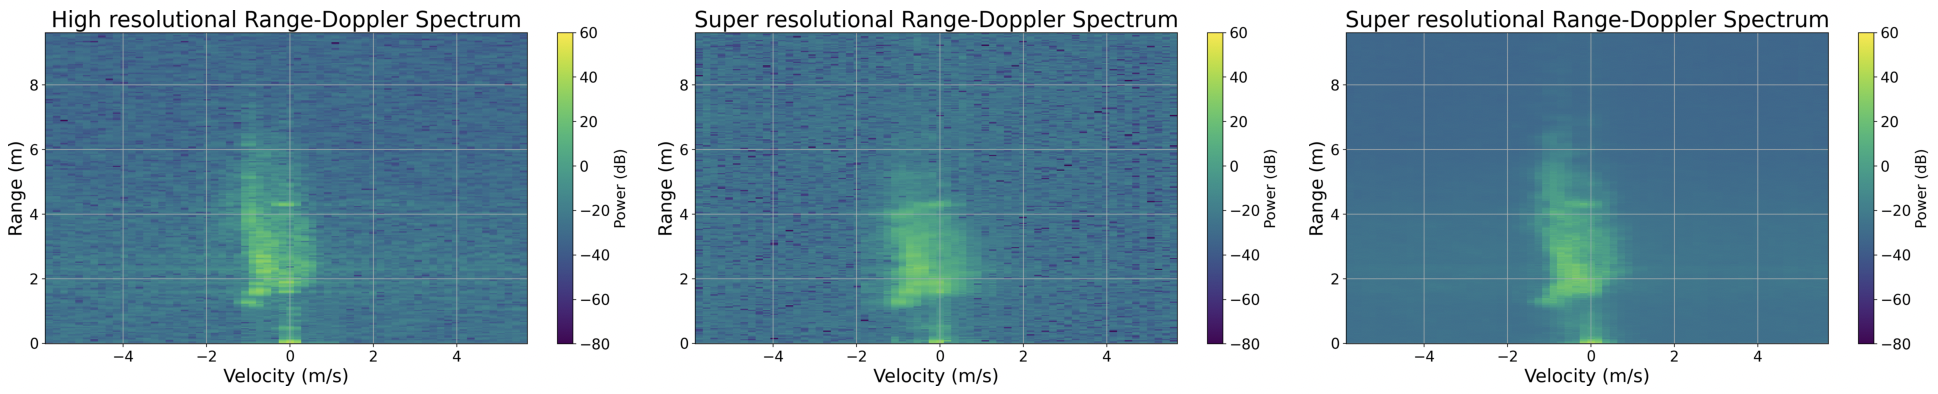
\includegraphics[scale=.34]{MA_presentation/figures/evaluation_processing_D_new.png}
        \caption{From left to right, high-resolution range-Doppler map, super-resolution range-Doppler maps of the cases without and with logarithm operation, respectively.}
        \label{super-resolution images of the logarithm types}
    \end{figure}
\end{frame}


\begin{frame}{Processing methods evaluation}
    \vspace{-1.5\baselineskip}
    \begin{table}
        \centering
        \small
        \caption{Evaluation losses of different amplitude normalization types}
        % \vspace{-2.5ex} 
        \label{Evaluation losses of the amplitude normalization types comparison in the case of no angle normalization}
        \vspace{-0.6cm}
        \begin{tabular}{l|c|c|c|c|c}
            \hline
            Amplitude normalization & MSE & SDR & LSD & WMSE & Perceptual \\
            \hline
            No normalization & 1.740 & \textbf{-9.251} & \textbf{0.295} & 0.130 & 17.636 \\
            \hline
            Normalization in (-1, 1) & 1.711 & -6.841 & 0.349 & \textbf{0.108} & 14.770 \\
            \hline
            Normalization in (0, 1) & \textbf{1.073} & -6.327 & 0.358 & 0.119 & \textbf{14.639} \\
            \hline
        \end{tabular}
    \end{table}

    \vspace{0.5\baselineskip}

    \begin{table}
        \centering
        \caption{Evaluation losses of the effect of the angle normalization type}
        \label{Evaluation losses of the angle normalization types comparison}
        \vspace{-0.65cm}
        \begin{tabular}{l|c|c|c|c|c}
            \hline
            Angle normalization & MSE & SDR & LSD & WMSE & Perceptual \\
            \hline
            No normalization & \textbf{1.073} & \textbf{-6.327} & \textbf{0.358} & 0.119 & \textbf{14.639} \\
            \hline
            With normalization & 1.330 & -6.068 & 0.363 & \textbf{0.117} & 15.204 \\
            \hline
        \end{tabular}
    \end{table}
\end{frame}


% \begin{frame}{Amplitude normalization types evaluation}
%     \begin{table}
%         \centering
%         \small
%         \caption{Evaluation losses of different amplitude normalization types}
%         \vspace{-2.5ex} 
%         \label{Evaluation losses of the amplitude normalization types comparison in the case of no angle normalization}
%         \begin{tabular}{l|c|c|c|c|c}
%             \hline
%             Amplitude normalization & MSE & SDR & LSD & WMSE & Perceptual \\
%             \hline
%             No normalization & 1.740 & \textbf{-9.251} & \textbf{0.295} & 0.130 & 17.636 \\
%             \hline
%             Normalization in (-1, 1) & 1.711 & -6.841 & 0.349 & \textbf{0.108} & 14.770 \\
%             \hline
%             Normalization in (0, 1) & \textbf{1.073} & -6.327 & 0.358 & 0.119 & \textbf{14.639} \\
%             \hline
%         \end{tabular}
%     \end{table}

%     \begin{figure}
%         \centering
%         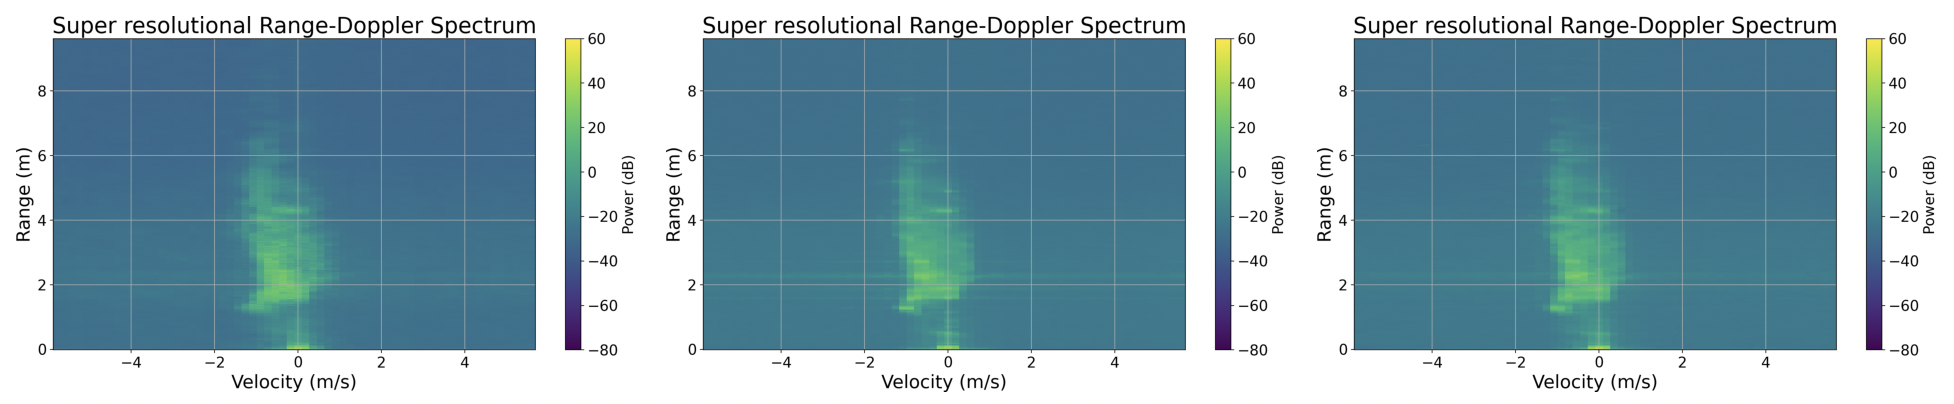
\includegraphics[scale=.34]{MA_presentation/figures/evaluation_processing_E.png}
%         \caption{Super-resolution images of different amplitude normalization types, from left to right, no amplitude normalization, normalization in (-1, 1) and normalization in (0, 1), respectively.}
%         \label{evaluation processing E}
%     \end{figure}
% \end{frame}


% \begin{frame}{Phase normalization types evaluation}
%     \begin{table}
%         \centering
%         \caption{Evaluation losses of the effect of the angle normalization type}
%         \vspace{-2.5ex} 
%         \label{Evaluation losses of the angle normalization types comparison}
%         \begin{tabular}{l|c|c|c|c|c}
%             \hline
%             Angle normalization & MSE & SDR & LSD & WMSE & Perceptual \\
%             \hline
%             No normalization & \textbf{1.073} & \textbf{-6.327} & \textbf{0.358} & 0.119 & \textbf{14.639} \\
%             \hline
%             With normalization & 1.330 & -6.068 & 0.363 & \textbf{0.117} & 15.204 \\
%             \hline
%         \end{tabular}
%     \end{table}

%     \begin{figure}
%         \centering
%         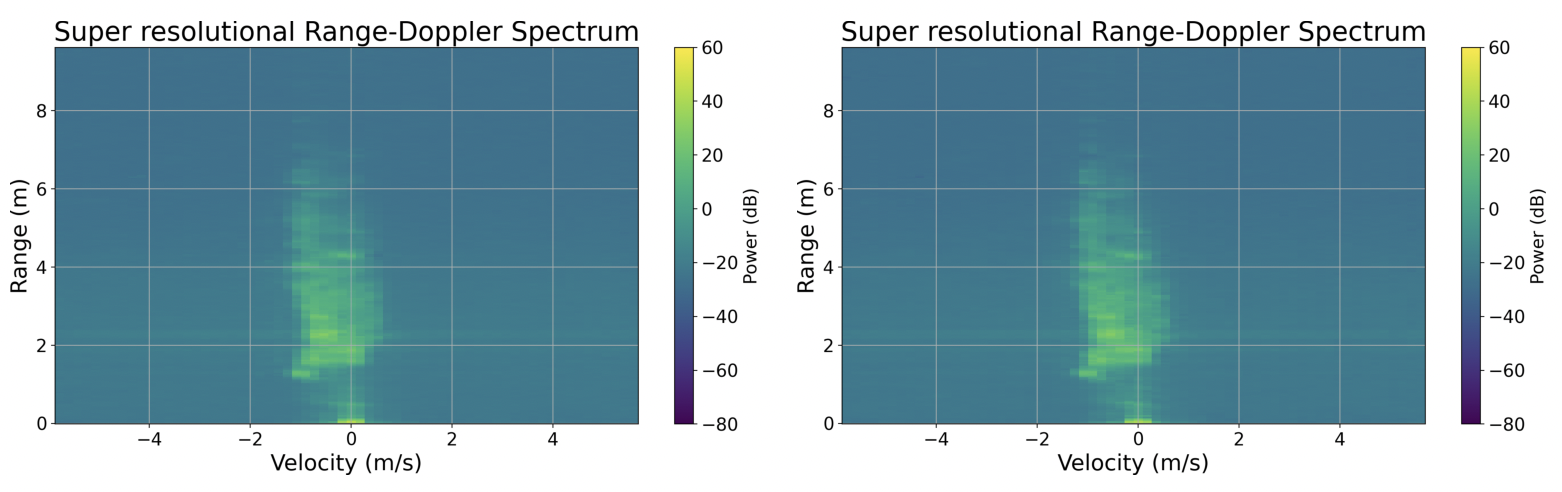
\includegraphics[scale=.34]{MA_presentation/figures/evaluation_processing_F_new.png}
%         \caption{Super-resolution images of the effect of the angle normalization type, left without angle normalization and right with angle normalization.}
%         \label{evaluation processing F}
%     \end{figure}
% \end{frame}


\begin{frame}{Training loss functions evaluation}
    \vspace{-1.5\baselineskip}
    \begin{table}
        \centering
        \caption{Evaluation losses of different training loss functions, horizontal axis is the evaluation loss functions, vertical axis is the training loss functions.}
        \label{Evaluation losses of the training loss functions comparison}
        \begin{tabular}{l|c|c|c|c|c}
            \hline
            Loss evaluation & MSE & SDR & LSD & WMSE & Perceptual \\
            \hline
            MSE & \textbf{1.073} & -6.327 & 0.358 & 0.119 & 14.639 \\
            \hline
            SDR & 1.110 & -5.683 & 0.370 & 0.121 & 14.163 \\
            \hline
            LSD & 1.232 & \textbf{-6.736} & \textbf{0.351} & \textbf{0.108} & 14.198 \\
            \hline
            PLSD & 1.424 & -6.434 & 0.356 & 0.124 & 16.999 \\
            \hline
            WMSE & 1.279 & -5.967 & 0.365 & 0.131 & 17.478 \\
            \hline
            Perceptual & 6.174 & -4.129 & 0.417 & 0.393 & \textbf{13.882} \\
            \hline
        \end{tabular}
    \end{table}
\end{frame}


\begin{frame}{Training loss functions evaluation}

    \begin{figure}
        \centering
        \vspace{-0.5\baselineskip}
        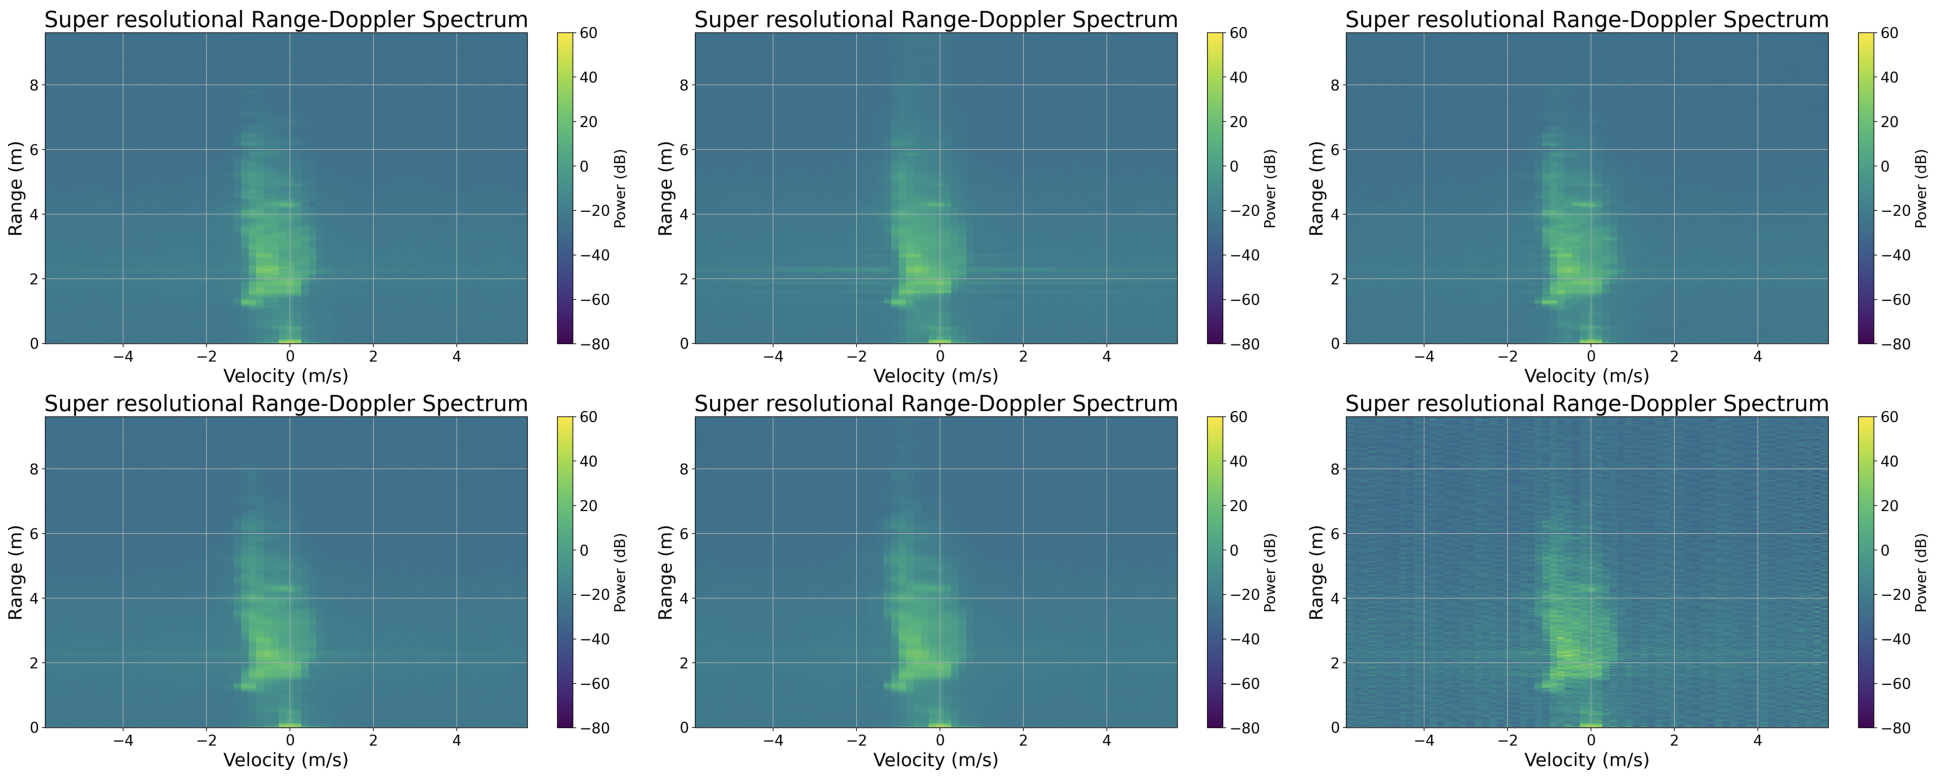
\includegraphics[scale=.33]{MA_presentation/figures/evaluation_loss_functions.png}
        \caption{Super-resolution range-Doppler maps of different training loss functions, from left to right, in the first row MSE, SDR and LSD, in the second row PLSD, WMSE and perceptual loss functions.}
        % \label{evaluation models 1}
    \end{figure}

    \vspace{-1.8\baselineskip}
    
    \begin{equation}
        \centering
        \mathcal{L}_{\text{Combination}} = \mathcal{L}_{\text{LSD}} + \lambda_c \times \mathcal{L}_{\text{Perceptual}} = \mathcal{L}_{\text{LSD}} + 0.5 \times \mathcal{L}_{\text{Perceptual}}
        \label{loss combination}
    \end{equation}
    
\end{frame}


% \begin{frame}{Loss combination evaluation}
%     \begin{table}
%         \centering
%         \caption{Evaluation losses of the training loss combination with different ratios.}
%         % \vspace{-2.5ex}
%         % \label{Evaluation losses of the training loss functions combination comparison}
%         \begin{tabular}{l|c|c|c|c|c}
%             \hline
%             LSD combination & MSE & SDR & LSD & WMSE & Perceptual \\
%             \hline
%             Lambda=1 & 2.464 & -5.270 & 0.383 & 0.220 & 13.779 \\
%             \hline
%             Lambda=0.5 & 1.731 & -5.375 & 0.380 & 0.179 & \textbf{12.320 }\\
%             \hline
%             Lambda=1e-1 & 1.347 & -5.829 & 0.369 & 1.150 & 12.979 \\
%             \hline
%             Lambda=1e-2 & 1.288 & -6.514 & 0.355 & 0.116 & 13.213 \\
%             \hline
%             Lambda=1e-3 & 1.486 & \textbf{-7.268} & \textbf{0.341} & \textbf{0.108} & 13.729 \\
%             \hline
%             Lambda=1e-4 & \textbf{1.265} & -6.405 & 0.357 & 0.115 & 14.138 \\
%             \hline
%         \end{tabular}
%     \end{table}
% \end{frame}


% \begin{frame}{Loss combination evaluation}
%     \begin{equation}
%         \centering
%         \mathcal{L}_{\text{Combination}} = \mathcal{L}_{\text{LSD}} + \lambda_c \times \mathcal{L}_{\text{Perceptual}}
%         \label{loss combination}
%     \end{equation}
    
%     \begin{figure}
%         \centering
%         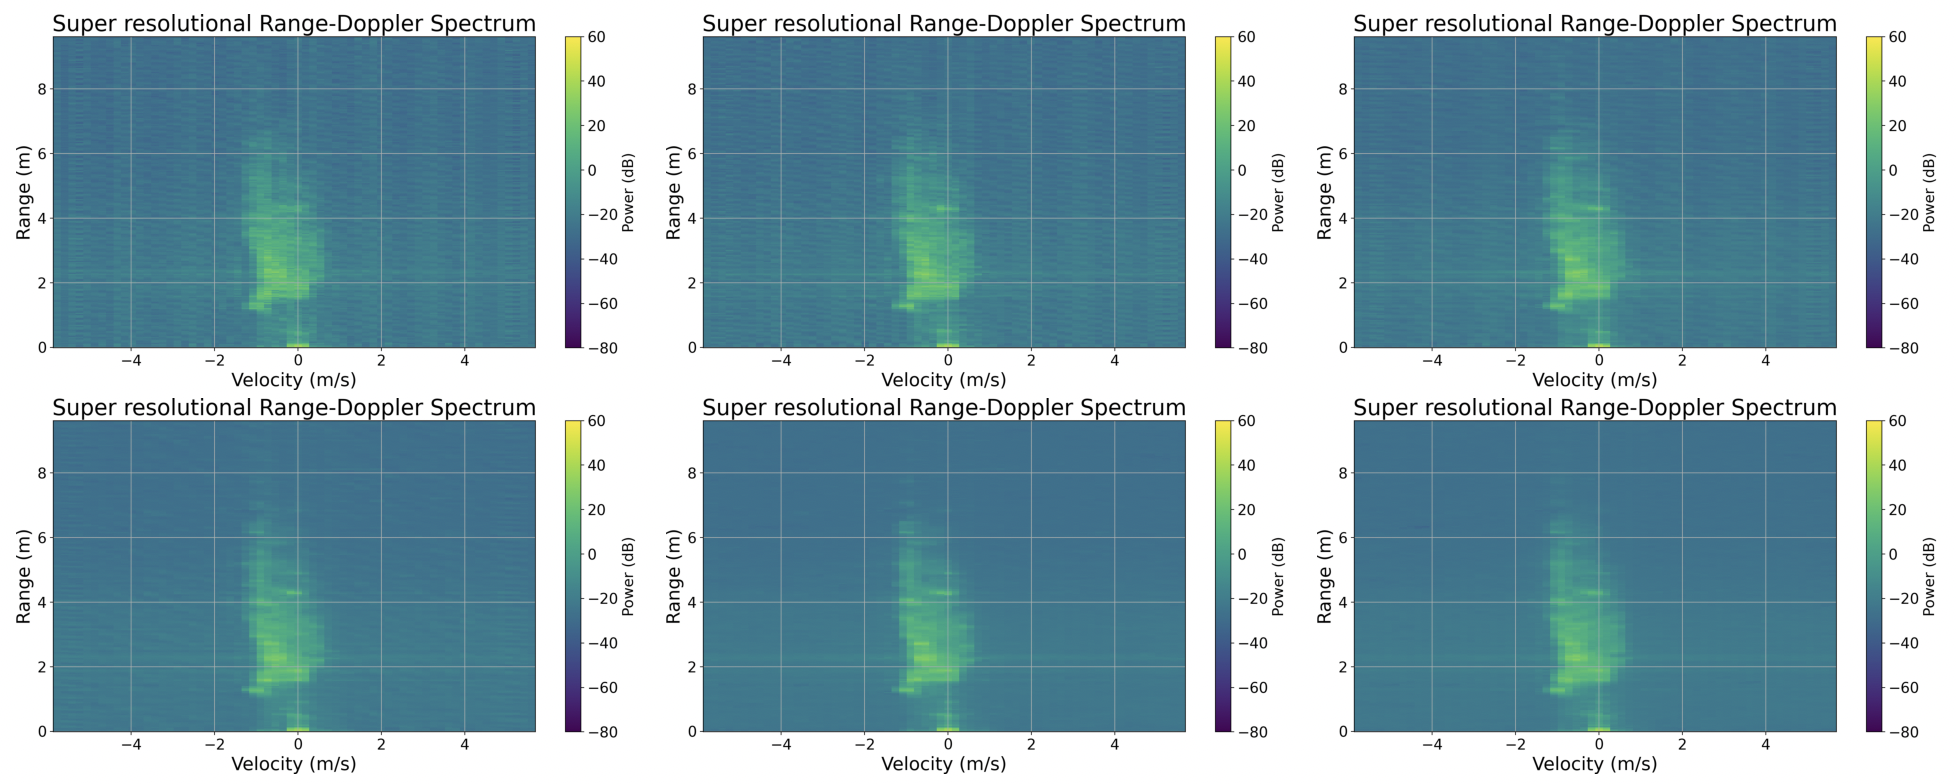
\includegraphics[scale=.33]{MA_presentation/figures/evaluation_loss_combination.png}
%         \caption{Super-resolution range-Doppler maps of the training loss combination with different ratios, from left to right, in the first row $\lambda_c$ as 1, 0.5 and 0.1, while in the second row 1e-2, 1e-3, 1e-4.}
%         \label{lsd+perceptual combination}
%     \end{figure}
% \end{frame}


% \begin{frame}{Models evaluation}
%     \begin{table}
%         \centering
%         \caption{Evaluation losses of different models in the case of the loss combination and new processing methods.}
%         % \vspace{-2.5ex}
%         % \label{models comparison in the case of the LSD and new processing methods}
%         \begin{tabular}{l|c|c|c|c|c}
%             \hline
%             Models & MSE & SDR & LSD & WMSE & Perceptual \\
%             \hline
%             Interpolation & 2.485 & -6.825 & 0.435 & 1.305 & 21.898 \\
%             \hline
%             CNN & 3.574 & -7.722 & 0.345 & 0.227 & 26.649 \\
%             \hline
%             UNet & 3.126 & -7.918 & 0.338 & 0.225 & 19.148 \\
%             \hline
%             UNet concat & 1.992 & \textbf{-8.355} & \textbf{0.320} & 0.175 & 17.916 \\
%             \hline
%             DP & 1.731 & -5.375 & 0.380 & 0.179 & \textbf{12.320 }\\
%             \hline
%             % DP & 2.052 & -5.530 & 0.377 & 0.192 & 11.997 \\
%             % \hline
%             SwinIR+DP & 1.662 & -6.415 & 0.360 & \textbf{0.128} & 16.903 \\
%             \hline
%             SwinIR+Swin & \textbf{1.619} & -6.392 & 0.360 & 0.134 & 15.662 \\
%             \hline
%         \end{tabular}
%     \end{table}
% \end{frame}


% \begin{frame}{Models comparison}
%     \begin{figure}
%         \centering
%         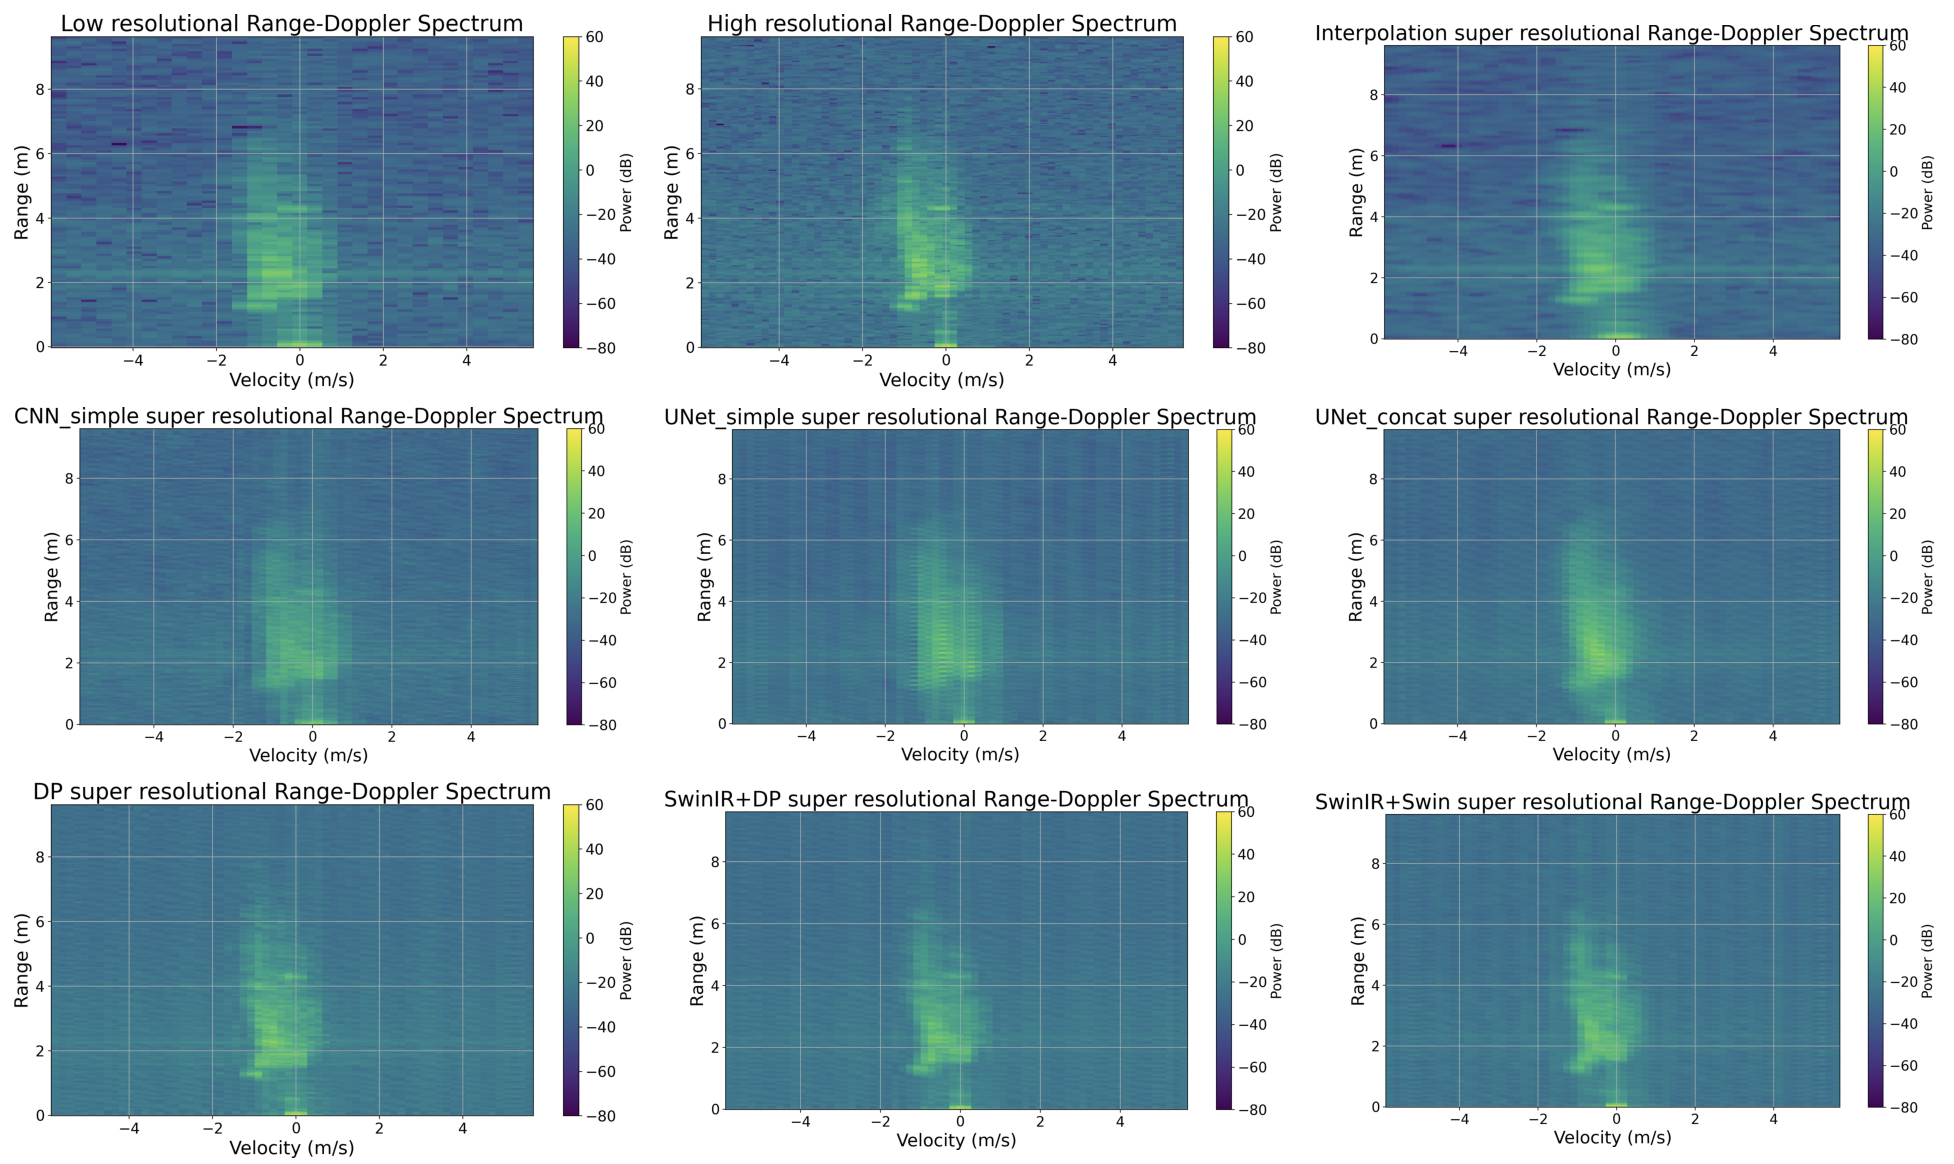
\includegraphics[scale=.3]{MA_presentation/figures/evaluation_models_2.png}
%         \caption{Range-Doppler maps in the case of loss combination and best processing methods, from left to right, first row: low-resolution, high-resolution, interpolation; the second row: CNN, UNet, UNet concat; third row: DP, SwinIR+DP, SwinIR+Swin.}
%         \label{evaluation models 2}
%     \end{figure}
% \end{frame}


\begin{frame}{cGAN evaluation}
    \begin{equation}
        \centering
        \mathcal{L}_{\text{Gen}} = \mathcal{L}_{\text{LSD}} + 0.5 \times \mathcal{L}_{\text{Perceptual}} + \lambda_g \times \mathcal{L}_{\text{GAN, Gen}}
        \label{loss combination}
    \end{equation}
    
    \begin{table}
        \centering
        \caption{Evaluation losses of cGAN model with and without low-resolution range-Doppler map compared with only generator, the \#Params of generator is 48,042 while that of discriminator is 76,267.}
        \label{Evaluation losses of FOL comparison}
        \begin{tabular}{l|c|c|c|c|c}
            \hline
            cGAN & MSE & SDR & LSD & WMSE & Perceptual \\
            \hline
            \multicolumn{6}{c}{With low-resolution input in discriminator}\\
            \hline
            $\lambda_g$=1e-2 & \textbf{1.339} & -5.103 & 0.385 & 0.177 & 11.926 \\
            \hline
            \multicolumn{6}{c}{Without low-resolution input in discriminator}\\
            \hline
            $\lambda_g$=1e-2 & 1.640 & \textbf{-5.690} & \textbf{0.374} & \textbf{0.169} & \textbf{11.881} \\
            \hline
            \multicolumn{6}{c}{Only generator}\\
            \hline
            DP & 1.731 & -5.375 & 0.380 & 0.179 & 12.320 \\
            \hline
        \end{tabular}
    \end{table}
\end{frame}


% \begin{frame}{cGAN evaluation}
%     \begin{equation}
%         \centering
%         \mathcal{L}_{\text{Gen}} = \mathcal{L}_{\text{LSD}} + 0.5 \times \mathcal{L}_{\text{Perceptual}} + \lambda_g \times \mathcal{L}_{\text{GAN, Gen}}
%         \label{loss combination}
%     \end{equation}

%     \begin{table}
%         \centering
%         \caption{Evaluation losses of the adversarial loss combination with different ratios in the case of the discriminator without low-resolution images as input.}
%         \label{Evaluation losses of the cGAN model comparison in the case of discriminator without low-resolution image as input}
%         \begin{tabular}{l|c|c|c|c|c}
%             \hline
%             cGAN & MSE & SDR & LSD & WMSE & Perceptual \\
%             \hline
%             Lambda=5e-1 & 1.802 & -5.216 & 0.383 & 0.186 & 13.543 \\
%             \hline
%             Lambda=1e-1 & 1.621 & -5.183 & 0.384 & 0.172 & 12.898 \\
%             \hline
%             Lambda=5e-2 & \textbf{1.447} & -5.463 & 0.379 & 0.181 & 13.311 \\
%             \hline
%             Lambda=1e-2 & 1.640 & -5.690 & 0.374 & \textbf{0.169} & \textbf{11.881} \\
%             \hline
%             Lambda=5e-3 & 1.525 & -5.305 & 0.382 & 0.193 & 12.956 \\
%             \hline
%             Lambda=1e-3 & 2.072 & \textbf{-5.845} & \textbf{0.370} & 0.182 & 14.396 \\
%             \hline
%         \end{tabular}
%     \end{table}
% \end{frame}


% \begin{frame}{cGAN evaluation}
%     \begin{figure}
%         \centering
%         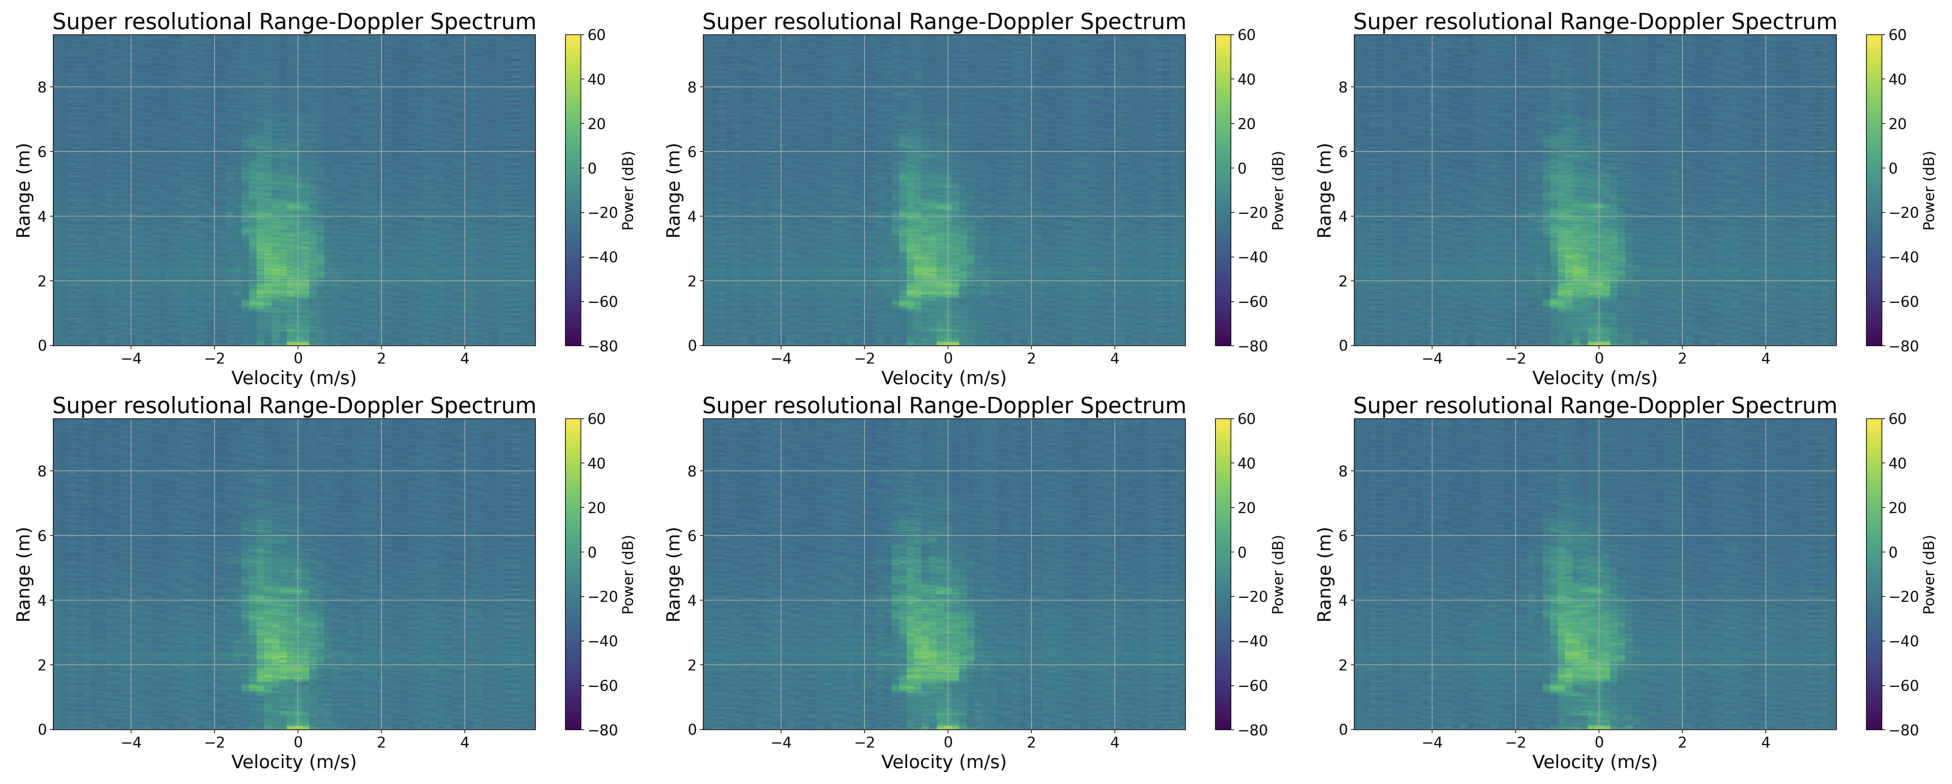
\includegraphics[scale=.33]{MA_presentation/figures/evaluation_cGAN_no_low_res.png}
%         \caption{Super-resolution images of the adversarial loss combination with different ratios in the case of the discriminator without low-resolution images as input, in the first row from left to right are lambda as 5e-1, 1e-1 and 5e-2, while in the second row from left to right 1e-2, 5e-3, 1e-3.}
%         \label{Super-resolution images of the cGAN model no low-res}
%     \end{figure}
% \end{frame}


% \begin{frame}{cGAN evaluation}
%     \begin{table}
%         \centering
%         \caption{Evaluation losses of the adversarial loss combination with different ratios in the case of the discriminator with low-resolution images as input.}
%         \label{Evaluation losses of the cGAN model comparison in the case of discriminator with low-resolution image as input}
%         \begin{tabular}{l|c|c|c|c|c}
%             \hline
%             cGAN & MSE & SDR & LSD & WMSE & Perceptual \\
%             \hline
%             Lambda=1e-1 & 1.592 & -5.361 & 0.381 & 0.164 & 13.861 \\
%             \hline
%             Lambda=5e-2 & 1.491 & -5.628 & \textbf{0.374} & \textbf{0.158} & 12.126 \\
%             \hline
%             Lambda=1e-2 & \textbf{1.339} & -5.103 & 0.385 & 0.177 & \textbf{11.926} \\
%             \hline
%             Lambda=5e-3 & 1.628 & -5.461 & 0.379 & 0.165 & 13.511 \\
%             \hline
%             Lambda=1e-3 & 1.920 & \textbf{-5.648} & 0.375 & 0.159 & 13.257 \\
%             \hline
%             Lambda=1e-4 & 3.593 & -5.331 & 0.381 & 0.190 & 14.148 \\
%             \hline
%         \end{tabular}
%     \end{table}
% \end{frame}


% \begin{frame}{cGAN evaluation}
%     \begin{figure}
%         \centering
%         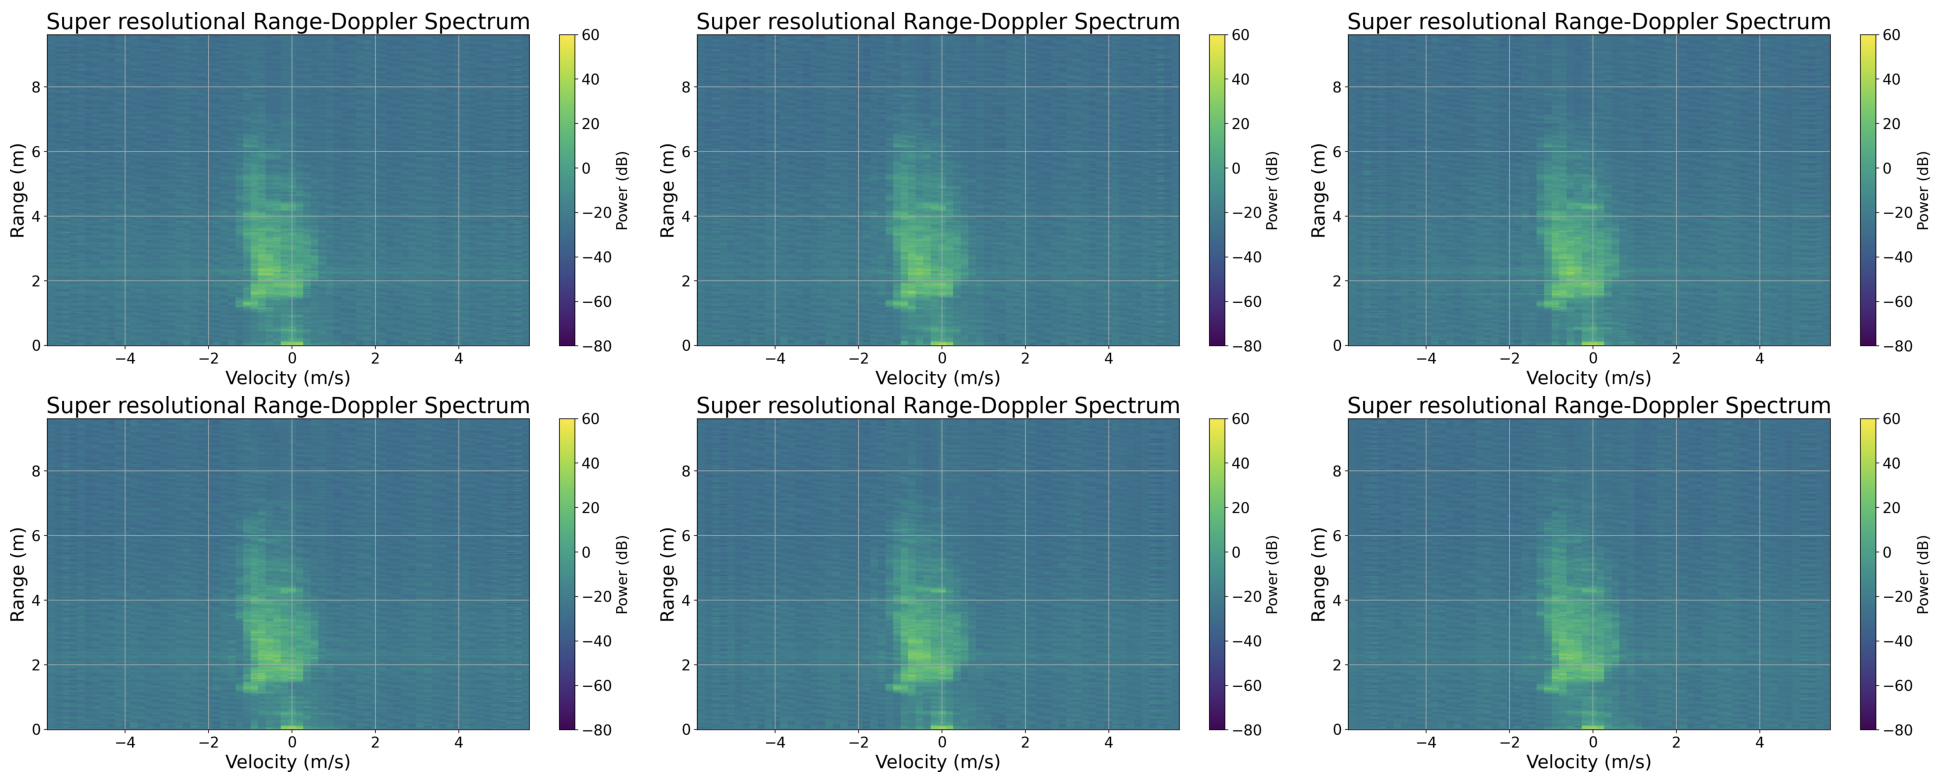
\includegraphics[scale=.33]{MA_presentation/figures/evaluation_cGAN_with_low_res.png}
%         \caption{Super-resolution images of the adversarial loss combination with different ratios in the case of the discriminator with low-resolution images as input, in the first row from left to right are lambda as 1e-1, 5e-2 and 1e-2, while in the second row from left to right 5e-3, 1e-3 and 1e-4.}
%         \label{Super-resolution images of the cGAN model with low-res}
%     \end{figure}
% \end{frame}


\begin{frame}{\#Frames evaluation}
    \vspace{-1.8\baselineskip}
    \begin{table}
        \centering
        \caption{Evaluation losses of different numbers of frames.}
        % \label{Evaluation losses of FOL comparison}
        \vspace{-0.5cm}
        \begin{tabular}{l|c|c|c|c|c}
            \hline
            \#Frames evaluation & MSE & SDR & LSD & WMSE & Perceptual \\
            \hline
            \multicolumn{6}{c}{\textbf{\#Frames = 1}}\\
            \hline
            DP & \textbf{1.379} & -5.239 & 0.381 & 0.191 & 12.778 \\
            \hline
            cGAN & 1.950 & -3.930 & 0.409 & 0.236 & 13.063 \\
            \hline
            \multicolumn{6}{c}{\textbf{\#Frames = 4}}\\
            \hline
            DP & 1.731 & \textbf{-5.375} & \textbf{0.380} & \textbf{0.179} & \textbf{12.320} \\
            \hline
            cGAN & \textbf{1.640} & \textbf{-5.690} & \textbf{0.374} & \textbf{0.169} & \textbf{11.881} \\
            \hline
        \end{tabular}
    \end{table}
\end{frame}


% \begin{frame}{FOL evaluation}
%     \begin{figure}
%         \centering

%         % Top row: two images side by side
%         \begin{minipage}{0.9\textwidth}
%             \centering
%             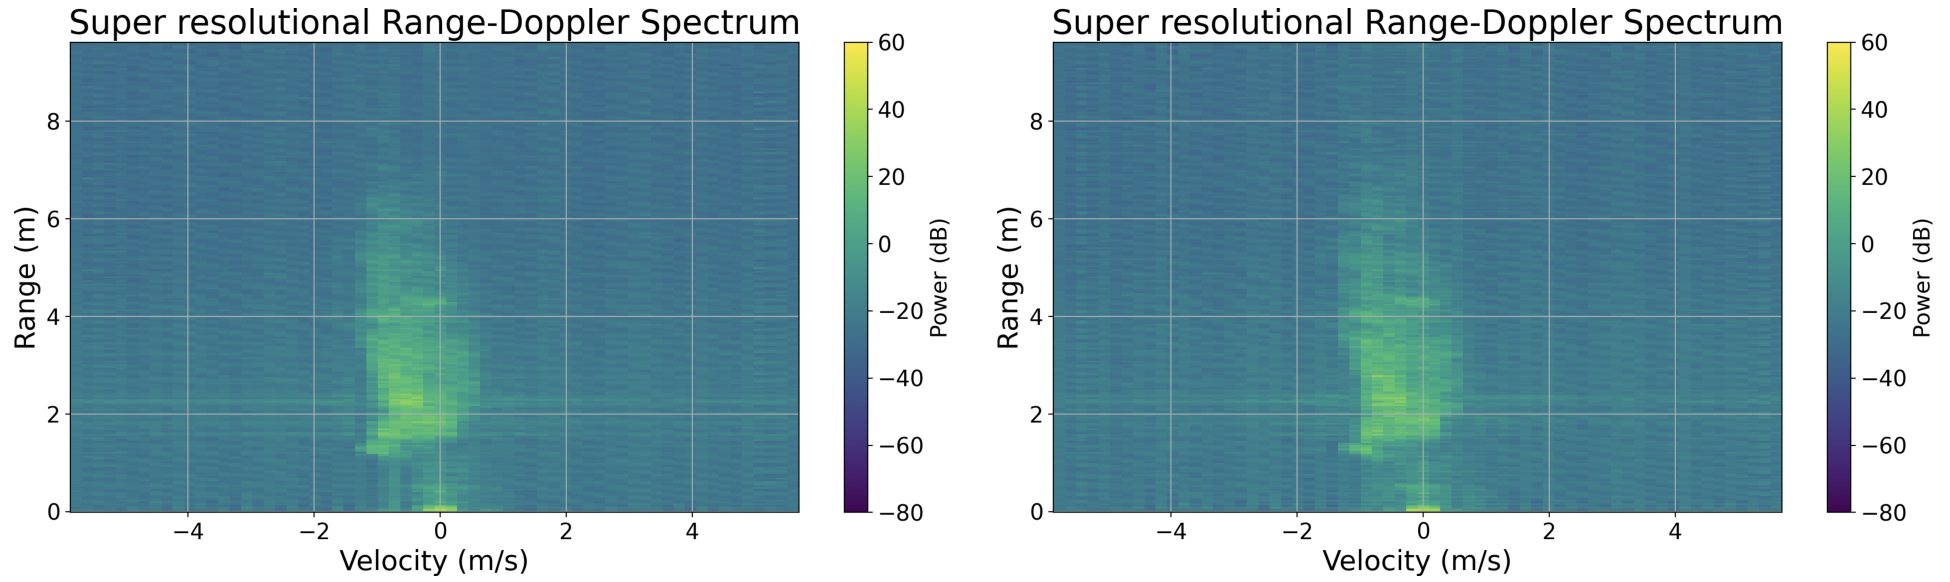
\includegraphics[width=\textwidth]{MA_presentation/figures/evaluation_FOL1_under.png}
%             % \small Masked high-resolution image
%         \end{minipage}

%         \vspace{0.1cm}

%         % Bottom image centered
%         \begin{minipage}{0.9\textwidth}
%             \centering
%             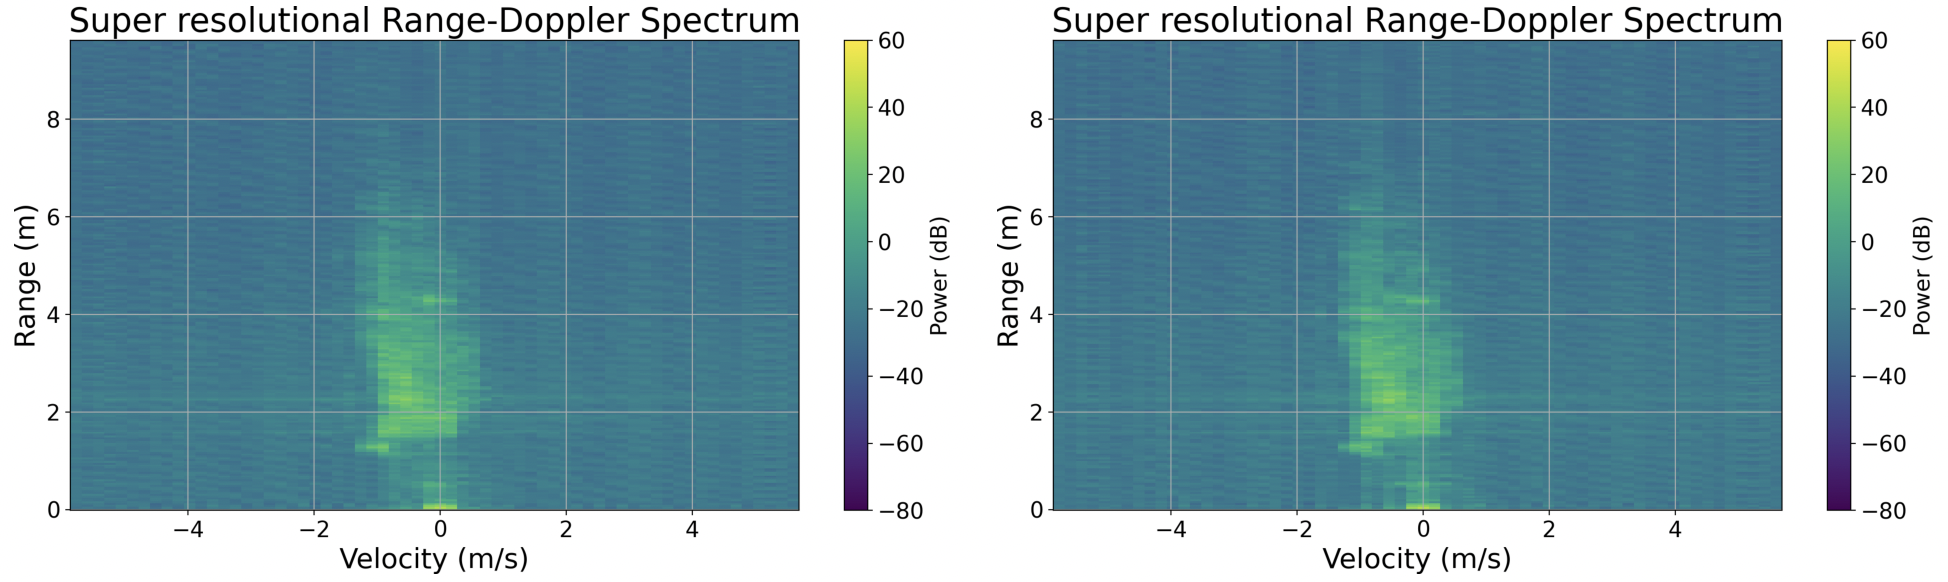
\includegraphics[width=\textwidth]{MA_presentation/figures/evaluation_FOL4_under.png}
%             % \small Masked high-resolution image
%         \end{minipage}

%         \caption{Super-resolution images of different FOL values, above are FOL as 1 while below are FOL as 4, left trained by DP-TF Transformer model and right trained by cGAN model.}
%     \end{figure}
    
% \end{frame}


% \begin{frame}{Resampling rate evaluation}
%     \begin{table}
%         \centering
%         \caption{Evaluation losses while the resampling rate as 4.}
%         \label{Evaluation losses while the resampling rate as 4}
%         \begin{tabular}{l|c|c|c|c|c}
%             \hline
%             Resampling rate & MSE & SDR & LSD & WMSE & Perceptual \\
%             \hline
%             DP & 2.208 & 5.811 & 0.620 & 0.491 & 22.347 \\
%             \hline
%             cGAN & 2.307 & 5.166 & 0.600 & 0.429 & 22.162 \\
%             \hline
%         \end{tabular}
%     \end{table}

%     \begin{figure}
%         \centering
%         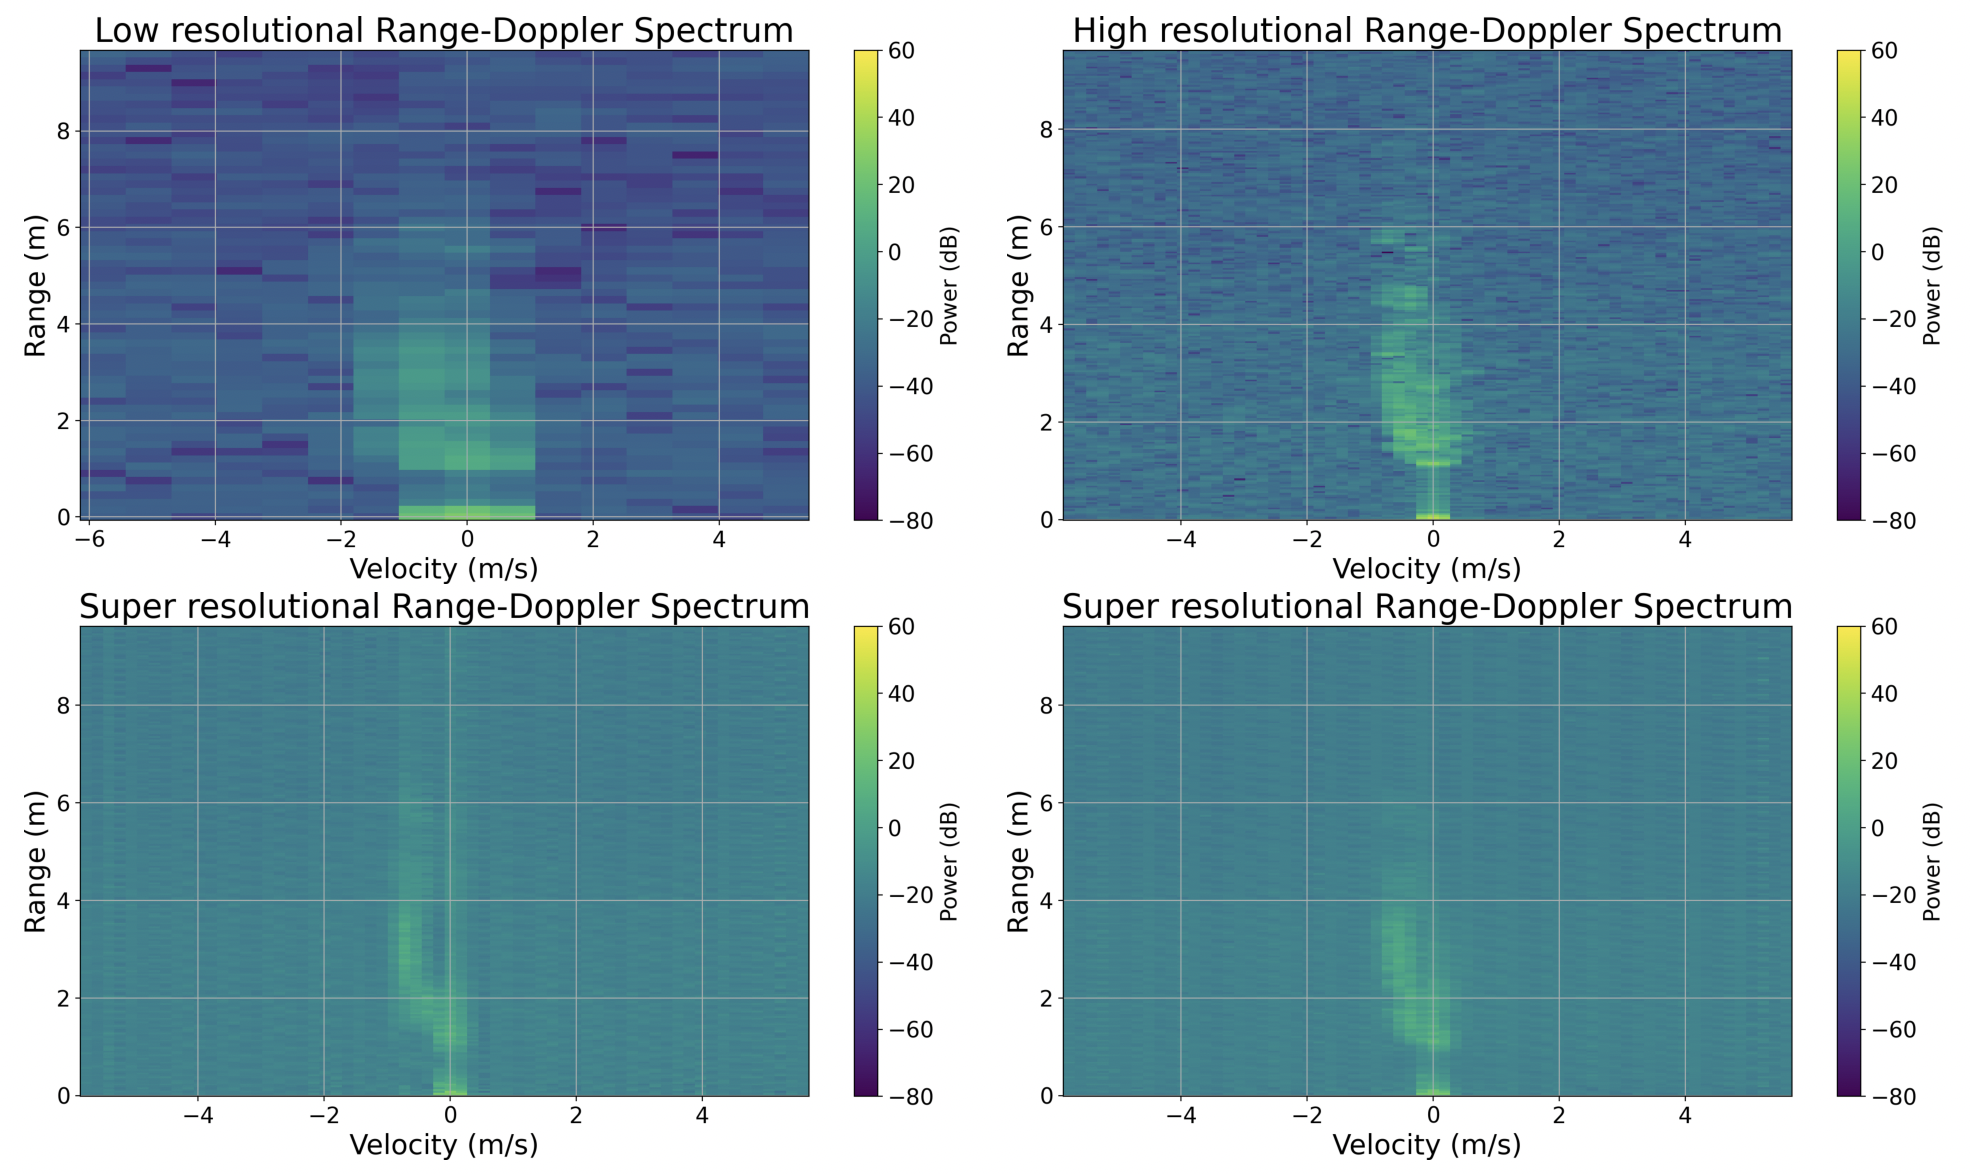
\includegraphics[scale=.22]{MA_presentation/figures/evaluation_resampling4.png}
%         \caption{Super-resolution images while the resampling rate as 4.}
%         \label{Super-resolution images while the resampling rate as 4}
%     \end{figure}
% \end{frame}


\begin{frame}{Hyperparameter tuning}
    \begin{figure}
        \hspace{-0.5cm}
        \centering
        \includegraphics[scale=.4]{MA_presentation/figures/evaluation_hyperparameters_tuning.png}
        \caption{Hyperparameter tuning by WandB \cite{wandb_site_2025}}
        \label{Hyperparameters tuning by WandB}
    \end{figure}

    % \begin{table}
    %     \centering
    %     \caption{Evaluation losses after hyperparameters tuning}
    %     \label{Evaluation losses after hyperparameters tuning}
    %     \begin{tabular}{l|c|c|c|c|c}
    %         \hline
    %         Tune & MSE & SDR & LSD & WMSE & Perceptual \\
    %         \hline
    %         DP & 1.225 & -5.625 & 0.373 & 0.146 & 11.753 \\
    %         \hline
    %         cGAN & 1.223 & -5.187 & 0.382 & 0.157 & 10.915 \\
    %         \hline
    %     \end{tabular}
    % \end{table}
\end{frame}


% \begin{frame}{Hyperparameters tuning}
%     \begin{figure}[!htp]
%         \centering
%         \includegraphics[scale=.3]{MA_presentation/figures/evaluation_tune.png}
%         \caption{Super-resolution images after the hyperparameters tuning, in the second row left on trained by DP-TF Transformer model while right one trained by cGAN model.}
%         \label{Super-resolution images after the hyperparameters tuning}
%     \end{figure}
% \end{frame}


\begin{frame}{Final result}
    % \begin{table}[!htp]
    %     \centering
    %     \caption{Evaluation losses with large models and whole dataset}
    %     \label{Evaluation losses with large models and whole dataset}
    %     \begin{tabular}{l|c|c|c|c|c}
    %         \hline
    %         Final result & MSE & SDR & LSD & WMSE & Perceptual \\
    %         \hline
    %         DP & 1.082 & -6.134 & 0.360 & 0.121 & \textbf{9.158} \\
    %         \hline
    %         cGAN & \textbf{1.016} & \textbf{-6.349} & \textbf{0.356} & \textbf{0.113} & 9.271 \\
    %         \hline
    %     \end{tabular}
    % \end{table}
    \vspace{-0.8\baselineskip}
    \begin{table}
        \centering
        \caption{Evaluation losses with large models and whole dataset, where the \#Params of generator is 329,410 and that of discriminator is 766,187.}
        \label{Evaluation losses with large models and whole dataset}
        \vspace{-0.2cm}
        \begin{tabular}{l|c|c|c|c|c}
            \hline
            Final result & MSE & SDR & LSD & WMSE & Perceptual \\
            \hline
            DP & 0.968 & \textbf{-6.008} & \textbf{0.363} & 0.123 & 9.079 \\
            \hline
            cGAN & \textbf{0.803} & -5.619 & 0.371 & \textbf{0.120} & \textbf{8.740} \\
            \hline
        \end{tabular}
    \end{table}
    \vspace{-0.2\baselineskip}
    \begin{figure}
        \centering
        \includegraphics[scale=.21]{MA_presentation/figures/evaluation_large_new.png}
        \vspace{-0.2cm}
        \caption{Super-resolution range-Doppler maps trained by large DP-TF Transformer and cGAN models with the whole dataset.}
        \label{Super-resolution images trained by large models and whole dataset}
    \end{figure}
\end{frame}



\begin{frame}[t]{Evaluation}
    \vspace{1.5\baselineskip}
	\begin{figure}
        % \vspace{0.5ex}
        \centering
        \hspace*{-1cm}
        \begin{minipage}{0.49\textwidth}
            \centering
            % \includegraphics[height=0.73\textwidth]{MA_presentation/gif_figures/epoch_201.jpg}
            \includegraphics[height=0.73\textwidth]{MA_presentation/gif_figures_testset/epoch_501.jpg}
            % \caption{High-resolution}
        \end{minipage}
        \begin{minipage}{0.49\textwidth}
            \centering
            % \animategraphics[height=0.73\textwidth, autoplay=True, loop=True]{10}{MA_presentation/gif_figures/epoch_}{1}{50}
            \animategraphics[height=0.73\textwidth, autoplay=True, loop=True]{12}{MA_presentation/gif_figures_testset/epoch_}{1}{80}
            % \caption{Super-resolution}
        \end{minipage}
        \caption{Visualization of range-Doppler map in the early epochs}
    \end{figure}
    
    % \begin{figure}
    %     \centering
    %     \animategraphics[width=0.5\linewidth, autoplay=True]{2}{MA_presentation/gif_figures/epoch_}{1}{101}
    %     \caption{Visualization of the training phase}
    % \end{figure}
\end{frame}



%% ===================================================================
\section{Summary \& Outlook}
\setcounter{section}{5}
\setcounter{figure}{0}
% --------------------------------------------------------------------

\begin{frame}{Summary}
    \begin{itemize}
        \item Dataset collection
        \vspace{0.5\baselineskip}
        \item DP-TF Transformer model with tuned hyperparameters
        \vspace{0.5\baselineskip}
        \item Processing methods
        \begin{itemize}
            \vspace{0.3\baselineskip}
            \item Amplitude and phase representation
            \vspace{0.3\baselineskip}
            \item Padding to deal with the range axis
            \vspace{0.3\baselineskip}
            \item Pixel shuffle layer to upsample
            \vspace{0.3\baselineskip}
            \item Logarithm and normalization on amplitude
        \end{itemize}
        \vspace{0.5\baselineskip}
        \item Loss combination with LSD and perceptual loss 
        \vspace{0.3\baselineskip}
        $\mathcal{L}_{\text{Combination}} = \mathcal{L}_{\text{LSD}} + 0.5 \times \mathcal{L}_{\text{Perceptual}}$
        \vspace{0.5\baselineskip}
        \item cGAN, where the generator is DP-TF Transformer model 
        \vspace{0.3\baselineskip}
        $\mathcal{L}_{\text{Gen}} = \mathcal{L}_{\text{LSD}} + 0.5 \times \mathcal{L}_{\text{Perceptual}} + 0.01 \times \| 1 - P_{\text{Super}} \|_{2}$
        % \vspace{0.5\baselineskip}
        % \item Resampling rate as 2
    \end{itemize}
\end{frame}



\begin{frame}{Outlook}
    \vspace{-1.2\baselineskip}
    \begin{itemize}
        \item Enrich the dataset further, such as more environments
        \vspace{0.5\baselineskip}
        % \item Fine-tuning on the hyperparameters
        % \vspace{0.5\baselineskip}
        \item More permutations and evaluations on the combination
        \vspace{0.5\baselineskip}
        \item Model optimization, such as division into different shapes
        \vspace{0.5\baselineskip}
        \item Other loss functions
    \end{itemize}
\end{frame}







%% ===================================================================
% Reference slide
\renewcommand*{\bibfont}{\tiny}
\begin{frame}[t]{Reference}
	\ifthenelse{\equal{\doclang}{german}}{
    	\bibliographystyle{IEEEtran_ISSger}
    }{
    	\bibliographystyle{IEEEtran_ISS}
    }
    \printbibliography{}
\end{frame}



%% ===================================================================
\begin{frame}[t]
    \centering
    \fontsize{24}{120}\selectfont
	\textbf{Thank you for your attention}
\end{frame}






















% %% =========
% \section{Firstsection}
% \subsection{First subsection}
% % -----------------------------------------------------------------------------
% \begin{frame}[t]{Slidetitle}
% \begin{itemize}
% 	\item Lorem:\\
% 	\begin{itemize}
% 		\item Ipsum
% 		\item Dolor
% 	\end{itemize}
% %	\item Methode:\\
% %	\begin{itemize}
% %		\item Angewandte Übungsaufgaben von Mathworks
% %		\item Überblicksvorlesung
% %		\item Betreute Einzelübungen am PC, geschulte Tutoren
% %	\end{itemize}
% 	\pause
% 	\item Sit amet, consectetur adipiscing elit:\\
% 	\begin{itemize}
% 		\item Phasellus ut est eget diam convallis porta.
% 		\item Ut dictum consequat sagittis.
% 		\item Cras laoreet sapien ut lectus sagittis et feugiat sapien interdum. 
% 	\end{itemize}
% 	\pause	
% 	\item In lorem purus, pulvinar in convallis ut, ullamcorper ac dolor.\\
% 	\begin{itemize}
% 		\item Sed nisi ligula, euismod sed consequat quis, euismod et quam
% 		\item Fusce mi mi, 
% 		\item ultricies
% 		\item vitae rhoncus sed,
% 	\end{itemize}			
% \end{itemize}		
	
% \end{frame}

% %% =========
% \subsection{Secondsection}
% % -----------------------------------------------------------------------------
% \begin{frame}[t]{Lorem Ipsum}
% 	\begin{itemize}	
% 		\item Lorem Ipsum
% 		\item dolor
% 		\item dolor
% 		\item dolor\\
% 	\begin{columns}[t,onlytextwidth]
% 		\column<2->{.5\textwidth}
% 		Pro:			
% 		\begin{itemize}
% 			\item Lorem Ipsum			
% 			\item Lorem Ipsum
% 			\item Lorem Ipsum
% 			\item ...
% 		\end{itemize}
% 		\column<3->{.5\textwidth}
% 		Contra:		
% 		\begin{itemize}
% 			\item Lorem Ipsum
% 			\item Lorem Ipsum
% 			\item Lorem Ipsum
% 			\item Lorem Ipsum
% 			\item ...
% 		\end{itemize}				
		
	
% 	\end{columns}
% 	\end{itemize}		
% \end{frame}

% %% =========
% \section{Third}
% % -----------------------------------------------------------------------------
% \begin{frame}[t]{Command Window}
% 	\begin{itemize}
% 		\item Prima 
% 		\item<2-> Secunda
% 	\end{itemize}

% 	\begin{figure}
% % 	\includegraphics<2->[height=0.4\textheight]{commandwindow.pdf}
% 	\end{figure}
% 	\only<3->{
% 	\begin{itemize}
% 		\item Tertia
% 		\item Quarta
% 	\end{itemize}
% 	}
% \end{frame}

% % -----------------------------------------------------------------------------
% \begin{frame}[t]{Quart}
% \begin{columns}[t,totalwidth=\textwidth]

% 	\begin{column}{0.7\textwidth}
	
% 		\begin{figure}
% 	 		%\includegraphics[width=\columnwidth]{file.png}
% 	 	\end{figure}	
	 	
% 	\end{column}
	
% 	\begin{column}{0.3\textwidth}
	
% 		\begin{itemize}
% 			\item Lorem
% 			\item Ipsum\\ \lstinline"code" 
% 			\item Dolor
% 		\end{itemize}
		
% 	\end{column}
	
% \end{columns}		
 	
% \end{frame}

% % -----------------------------------------------------------------------------
% \subsection{SubSectiones}
% \begin{frame}[t]{SubSectiones}
% \pause
% Definitium est\\
% \flushright{Caesar}
% 	\begin{itemize}
% 			\item Lorem
% 				\begin{itemize}
% 					\item Ipsum
% 					\item ...
% 					\item ...
% 					\item ...
% 				\end{itemize}
% 			\pause
% 			\item Code:\\
% 				\lstinline"A!=B"\\
% 				\lstinline"A & B"\\
% 				\lstinline"define C"\\
% 				~~~~\lstinline"result"
% 	\end{itemize}
% \end{frame}

\end{document}